
%****Header*****

\documentclass[%draft,
fleqn,											%richtet die Formel links aus, Einzug wird unten definiert
12pt,a4paper,
%twoside,openright,					%fuer einseitigen Druck diese beiden Optionen auskommentieren und unten ensprechende Kopfzeilenoption waehlen (bis ca 120 Seiten)
bibliography=totoc,listof=totoc,BCOR=5mm,
ngerman
%english
]{scrreprt}

%%%%%%%%%%%%%%%%%%%%%%%%%%%%%%%%%%%%%%%%%%%
%Textliches und sprachliches
%%%%%%%%%%%%%%%%%%%%%%%%%%%%%%%%%%%%%%%%%%%
\usepackage[T1]{fontenc}		% die beiden Packete geh�ren zusammen, um Umlaute und �hnliche deutsche "Sonderzeichen"
\usepackage[latin1]{inputenc} %direkt eingeben zu k�nnen
\usepackage[english]{babel}%kommt es zu einer Uebersetzung der sprachspezifischen Befehle im Dokument (�Inhaltsverzeichnis� statt �table of contents�, �Kapitel� anstelle von �chapter� usw.) und fuer korrekte Trennung wichtig
\usepackage{upgreek} 				%erlaubt die Eingabe von aufrechten griechischen Kleinbuchstaben
\pagestyle{headings} 				%schaltet die Kopfzeile ein. Die Option {headings} erzeugt die Nummer und den Namen des Kapitels
\usepackage{setspace} 			%enth�lt u.a. den Befehl \onehalfspacing, der daf�r sorgt, dass 1 1/2 Zeilen Abstand gelassen wird zwischen zwei Zeilen
\usepackage{rotating}
\usepackage{pdflscape}
\usepackage[]{nomencl}  % Nomenclature Symbolverzeichnis
\usepackage[euler]{textgreek}
%%%%%%%%%%%%%%%%%%%%%%%%%%%%%%%%%%%%%%%%%%%
%Verzeichnisse
%%%%%%%%%%%%%%%%%%%%%%%%%%%%%%%%%%%%%%%%%%%
\setcounter{secnumdepth}{2} %bestimmt, in welcher Tiefe Ueberschriften noch nummeriert werden. 5 Steht dafuer, dass alle Ueberschriften nummeriert werden
\setcounter{tocdepth}{1} 		%Bestimmt die Nummerierungstiefe im Inhaltsverzeichnis
\usepackage{cite}						%braucht man f�rs Literaturverzeichnis
\usepackage{bibgerm} 				%F�r die Literaturverzeichniserstellung auf deutsch
\usepackage{epstopdf}			% F�r eps Bilder
%%%%%%%%%%%%%%%%%%%%%%%%%%%%%%%%%%%%%%%%%%%
%Mathematisches
%%%%%%%%%%%%%%%%%%%%%%%%%%%%%%%%%%%%%%%%%%%
\usepackage{amssymb,amsfonts,amsmath} %Eingabehilfen f�r Formeln
\usepackage{siunitx} 				%erlaubt die Eingabe von Einheiten, so dass die Einheit und der Wert schoen zusammenstehen und nicht getrennt werden beim Zeilenumbruch.

%%%%%%%%%%%%%%%%%%%%%%%%%%%%%%%%%%%%%%%%%%%
%Bildtechnisches
%%%%%%%%%%%%%%%%%%%%%%%%%%%%%%%%%%%%%%%%%%%
\usepackage{graphicx} 			%um Bilder einzubinden
\usepackage[table]{xcolor}
\usepackage{float} 		%erlaubt mehr float Objekte (z.B. Bilder oder Tabellen) auf einer Seite
%\usepackage{subfig}				%wenn mehrere Bilder unter einer Caption zusammengefasst werden sollen
\usepackage[center,small,bf]{caption} %gibt die Optionen f�r das Verhalten der Bildunterschriften (caption) an, muss nach Paketen wie subfig, float, rotating eingebunden werden

%%%%%%%%%%%%%%%%%%%%%%%%%%%%%%%%%%%%%%%%%%%
%Fuss- und Kopfzeilendefinition
%%%%%%%%%%%%%%%%%%%%%%%%%%%%%%%%%%%%%%%%%%%
\usepackage{fancyhdr}
\fancyhead{}
\fancyfoot{}
\renewcommand{\headrulewidth}{0.5pt}

%%% zweiseitiges Seitenlayout
%\fancyhead[EL, OR]{ \thepage}
%\fancyhead[EC]{\textsl{\leftmark}}
%\fancyhead[OC]{\textsl{\rightmark}}
%%% Ende: zweiseitiges Seitenlayout

%%% einseitiges Seitenlayout
\fancyhead[R]{ \thepage}
\fancyhead[C]{\textsl{\leftmark}}
%%% Ende: einseitiges Seitenlayout

\pagestyle{fancy}

\renewcommand{\chaptermark}[1]{%
\markboth{\thechapter\ #1}{}}

\renewcommand{\sectionmark}[1]{%
\markright{\thesection\ #1}}

%------------------------------------------------------------------------------
%Bis hierhin darf der Header nur in Ruecksprache mit dem Betreuer geaendert werden.
%------------------------------------------------------------------------------

%%%%%%%%%%%%%%%%%%%%%%%%%%%%%%%%%%%%%%%%%%%
%Definitionen f�r siunitx-Paket
%wird nur in deutscher Version benoetigt
%%%%%%%%%%%%%%%%%%%%%%%%%%%%%%%%%%%%%%%%%%%
\sisetup{locale=DE} 			%macht, dass statt Punkt ein Komma als Dezimaltrenner verwendet wird
\sisetup{%
  list-final-separator = { \translate{and} },
  range-phrase = { \translate{to (numerical range)} }
} 												%macht dass in Liste und Range die Woerter richtig uebersetzt werden

%%%%%%%%%%%%%%%%%%%%%%%%%%%%%%%%%%%%%%%%%%%
%Einbinden mehrseitiger PDFs oder Ausschnitte daraus
%%%%%%%%%%%%%%%%%%%%%%%%%%%%%%%%%%%%%%%%%%%
%\usepackage{calc}
%\usepackage{eso-pic}
%\usepackage{everyshi}
%\usepackage{pdfpages}

%%%%%%%%%%%%%%%%%%%%%%%%%%%%%%%%%%%%%%%%%%%
%Fuer das Erstellen von Bildern aus Matlab mit \psfragfig
%%%%%%%%%%%%%%%%%%%%%%%%%%%%%%%%%%%%%%%%%%%
%Fuer die Nutzung von \psfragfig muessen die Bilder mit Hilfe des figures_fuer_latex.m erzeugt werden -- es muss dem Complier noch das Argument "-shell-escape" uebergeben werden (bei Texniccenter Alt+F7)
%\usepackage{pstool}
\usepackage[crop=pdfcrop]{pstool} %verschmaelert die Raender der Abbildung
%\usepackage[cleanup={}]{pstool} 	 %log-Datei bleibt erhalten: zum Debuggen

%%%%%%%%%%%%%%%%%%%%%%%%%%%%%%%%%%%%%%%%%%%
%Fuer den Import von Bildern aus Inkscape
%%%%%%%%%%%%%%%%%%%%%%%%%%%%%%%%%%%%%%%%%%%
%\graphicspath{{figures/}}
%\newcommand{\executeiffilenewer}[3]{%
%\ifnum\pdfstrcmp{\pdffilemoddate{#1}}%
%{\pdffilemoddate{#2}}>0%
%{\immediate\write18{#3}}\fi%
%}
%\newcommand{\includesvg}[1]{%
%\executeiffilenewer{#1.svg}{#1.pdf}%
%{inkscape -z -D --file=#1.svg %
%--export-pdf=#1.pdf --export-latex}%
%\input{#1.pdf_tex}%
%}

%%%%%%%%%%%%%%%%%%%%%%%%%%%%%%%%%%%%%%%%%%%
%Fuer TpX
%Mit TpX koennen unter Window recht einfach Diagramme erstellt werden
%%%%%%%%%%%%%%%%%%%%%%%%%%%%%%%%%%%%%%%%%%%
%\usepackage{color,ifpdf,graphicx}
%\ifpdf %if using PDFTeX in PDF mode
%  \DeclareGraphicsExtensions{.pdf,.png,.mps}
%\else %if using TeX or PDFTeX in TeX mode
%  \DeclareGraphicsExtensions{.eps,.bmp}
%  \DeclareGraphicsRule{.emf}{bmp}{}{}% declare EMF filename extension
%  \DeclareGraphicsRule{.png}{bmp}{}{}% declare PNG filename extension
%  \usepackage{pstricks}%variant: \usepackage{pst-all}
%\fi
%\usepackage{pgf,epic,bez123,floatflt,wrapfig}

%%%%%%%%%%%%%%%%%%%%%%%%%%%%%%%%%%%%%%%%%%%
%Neu-/Umdefinitionen
%%%%%%%%%%%%%%%%%%%%%%%%%%%%%%%%%%%%%%%%%%%
\usepackage[pdfborder={0 0 0}, breaklinks=true]{hyperref} %muss als letztes Paket eingebunden werden, verlinkt Referenzen, so dass im pdf direkt zu der Stelle gesprungen wird

%%%%%%%%%%%%%%%%%%%%%%%%%%%%%%%%%%%%%%%%%%%
%Neu-/Umdefinitionen
%%%%%%%%%%%%%%%%%%%%%%%%%%%%%%%%%%%%%%%%%%%

\newcommand{\sfs}{SF$_6$} 
%% ----------------------------------------------------------------
% Aus AMS
% ----------------------------------------------------------------

\newcommand{\titlestring}{{Berechnung und Reduktion der tonalen
Ger�uschemission von Hochspannungsfreileitungen}}

\newcommand{\UnterTitlestring}{{Berechnung und Massnahmen zu deren
Reduktion}}

\newcommand{\DissNummer}{{17408}}
\newcommand{\degreestring}{{Doktor der Wissenschaften}}
\newcommand{\authorstring}{{Ulrich Straumann}}
\newcommand{\acadtitlestring}{{Dipl.-Phys. Universit�t Z�rich}}
\newcommand{\dateofbirthstring}{{11. Januar 1975}}
\newcommand{\citizenstring}{{Fehren SO und Oberg�sgen SO}}
\newcommand{\examinerstring}{Prof. Dr. K. Fr�hlich}
\newcommand{\coexaminerstring}{Prof. Dr. E. Gockenbach, Korreferent \\ Dr. K. Heutschi}

\EndPreamble
\begin{document}

	\pagenumbering{roman} 		%Schaltet die Seitenzahlen auf roemische Zahlen

%	\begin{titlepage}
\setlength{\baselineskip}{8mm}
{\large\noindent DISS.\ ETH Nr.\ \DissNummer}
\vfill
\begin{center}
  {\def\\{\linebreak}
  \huge\bf\titlestring}
\end{center}
\vfill
\begin{center}
  \large ABHANDLUNG \linebreak
  zur Erlangung des Titels \linebreak
  \degreestring
\end{center}
\vspace{0.5\fill}
\begin{center}
  \large der \linebreak
  EIDGEN�SSISCHEN TECHNISCHEN HOCHSCHULE \linebreak
  Z�RICH
\end{center}
\vspace{0.5\fill}
\begin{center}
  \large vorgelegt von \vspace{5mm}  \linebreak %NK
  \textsc{\authorstring} \vspace{5mm} \linebreak  %NK
  \acadtitlestring \linebreak
  geboren am \dateofbirthstring \linebreak
  von \citizenstring
\end{center}
\vspace{0.5\fill}
\begin{center}
  \large Angenommen auf Antrag von: \linebreak
  \examinerstring, Referent \linebreak
  \coexaminerstring, Korreferent
\end{center}
\vspace{0.5\fill}
\begin{center}
  \large\number\year
\end{center}
\end{titlepage}

	

%**** Titelseite *****

\pagestyle{empty}

\begin{figure}
    \begin{minipage}[b]{0.5\linewidth}
        
\includegraphics[width=0.8\textwidth]{figures/ethlogo}
    \end{minipage}
    \hfill
    \begin{minipage}[b]{0.45\linewidth}
        \flushright
        \textbf{High Voltage Laboratory}\\
        \vspace{3mm}
        Prof. Dr. Christian Franck
    \end{minipage}
\end{figure}


\begin{flushright}
    \textit{ETH Z�rich\\
    Physikstr. 3, ETL\\
    8092 Zurich\\
    Switzerland}
\end{flushright}

\phantom{u}
\vspace{1.5cm}
\Huge{\sc Feasibility study on the use of current transformers in dielectric spectroscopy}
\vspace{1.5cm}

\Large
GROUP PROJECT, SEMESTER PROJECT\\

\vspace*{5cm} \large
Deuschle Leonard, Philipp, Aron

dleonard@ethz.ch, philipar@ethz.ch

\normalsize

\vspace{1.5cm}

Supervisor: Raphael F\'arber

Autumn Semester 2015
	\cleardoublepage					%notwendig, damit keine Seitenzahl auf Titelseite

%%%%%%%%%%%%%%%%%%%%%%%%%%%%%%%%%%%%%%%%%%%%%%%%%%%%%%%%%%%%%%%%%%%%%%%%%%%%%%%%
%Vorspann
%%%%%%%%%%%%%%%%%%%%%%%%%%%%%%%%%%%%%%%%%%%%%%%%%%%%%%%%%%%%%%%%%%%%%%%%%%%%%%%%
	\pagestyle{fancy}
	
	
<<<<<<< HEAD
\begin{center}
  \makebox[\textwidth]{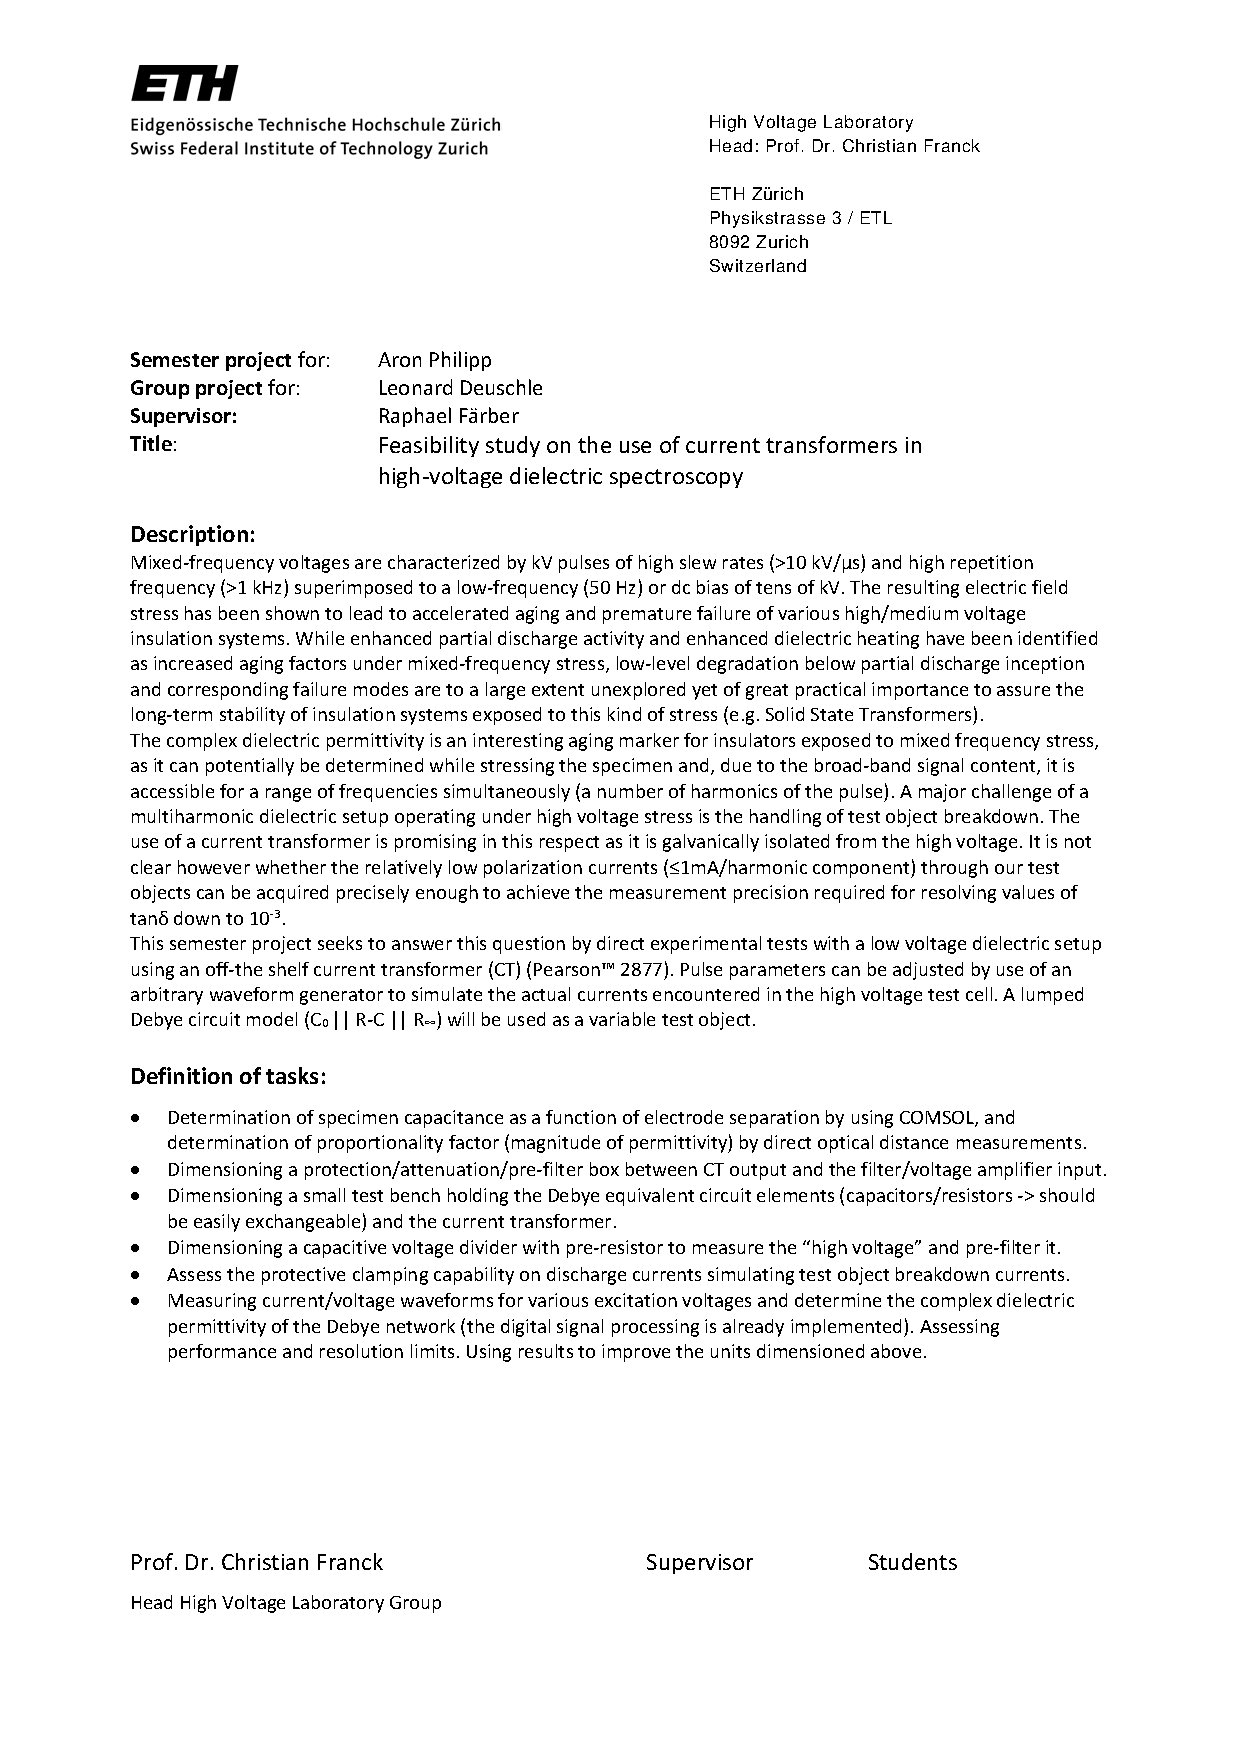
\includegraphics[width=\paperwidth, height=\paperheight]{figures/Project_Definition_Philipp_Deuschle_HS15.pdf}}
=======
\chapter*{Aufgabenstellung}



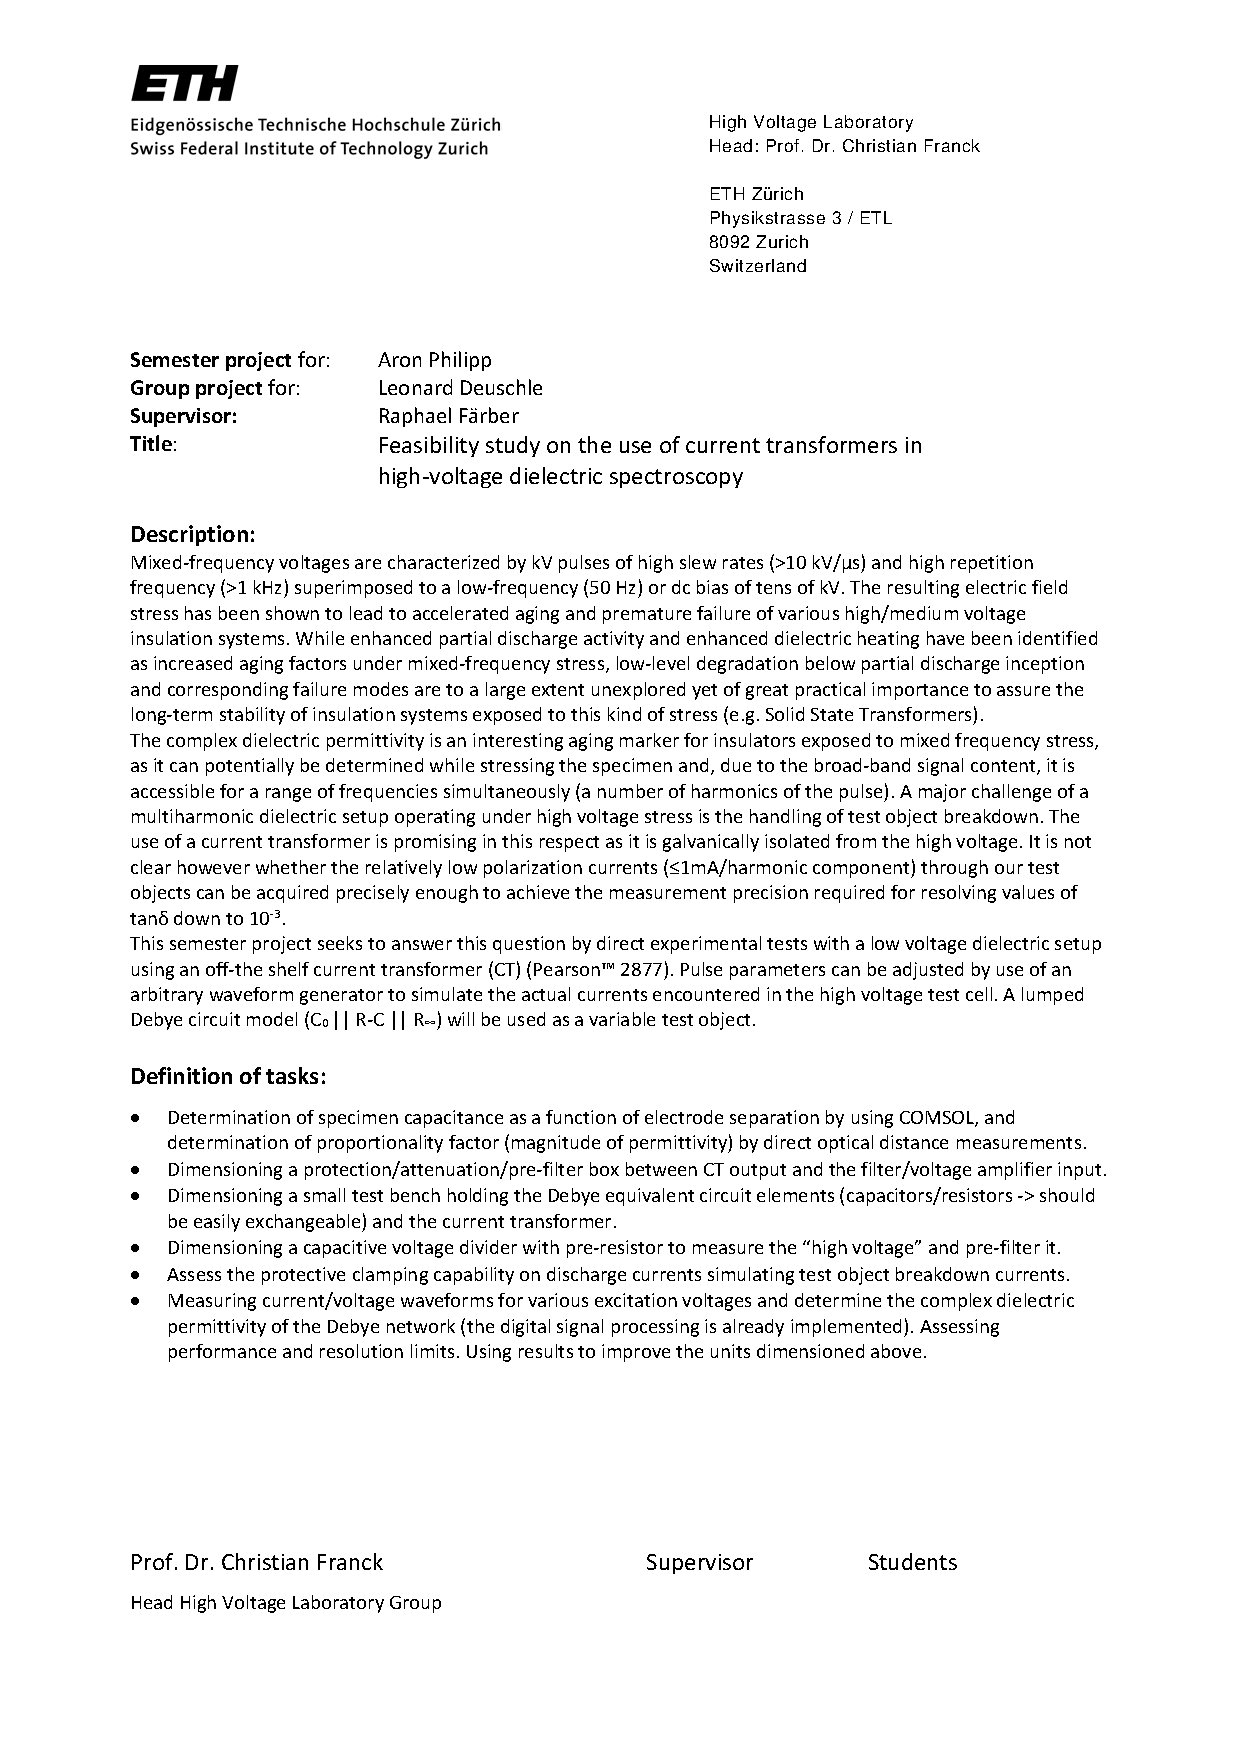
\includegraphics{figures/Project_Definition_Philipp_Deuschle_HS15.pdf}
>>>>>>> 0d939384617ec4e70e21752a52b662e06c59e28a

%	
\chapter*{Kurzfassung}

Der Zweck der Kurzfassung ist, die wesentlichen Informationen und Konsequenzen aus der Arbeit dem Leser in kurzer Form anzubieten. Sie soll daher folgendermassen aufgebaut werden:
\begin{enumerate}
    \item Problemstellung (inkl. Hintergrund)
    \item Innovation / Neue Elemente
    \item Methode / L�sungswege
    \item Wesentliche Resultate
    \item Schlussfolgerungen
    \item Konsequenzen f�r die Fachwelt, das Projekt oder weitere Arbeiten
\end{enumerate} 
	\input{text/abstract}

	\tableofcontents 				%erzeugt das Inhaltsverzeichnis

	\cleardoublepage 				%notwendig, damit arabische Nummerierung erst beim ersten Kapitel beginnt
	\pagenumbering{arabic} 	%Schaltet die Seitenzahlen auf arabische Zahlen
%	\onehalfspacing

%%%%%%%%%%%%%%%%%%%%%%%%%%%%%%%%%%%%%%%%%%%%%%%%%%%%%%%%%%%%%%%%%%%%%%%%%%%%%%%%
%Hauptteil
%%%%%%%%%%%%%%%%%%%%%%%%%%%%%%%%%%%%%%%%%%%%%%%%%%%%%%%%%%%%%%%%%%%%%%%%%%%%%%%%

	\input{text/abstract}
	%
	
\chapter{Introduction}
Power electronics systems, especially converters, lead to a more complex electrical field stress in insulation material of energy transmission systems as it introduces pulses (>1 kV) with high slew rates (>$10 \frac{kV}{\mu s}$) and high repetition frequencies (> 1 kHz) superimposed on low frequencies (50 Hz) or DC. The latter can cause enhanced partial discharges (PD) in the insulation system, i.e. a breakdown of a part of the insulation system. \cite{TransformerEngineering}. However, there are already effects below partial discharge inception that are not well understood, yet. They do as well result in an accelerated aging of the insulation due to the sustained application of the converter pulses. 
\newline

\begin{figure}[!ht]
  \begin{minipage}{0.5\textwidth}
  

  
  \centerline{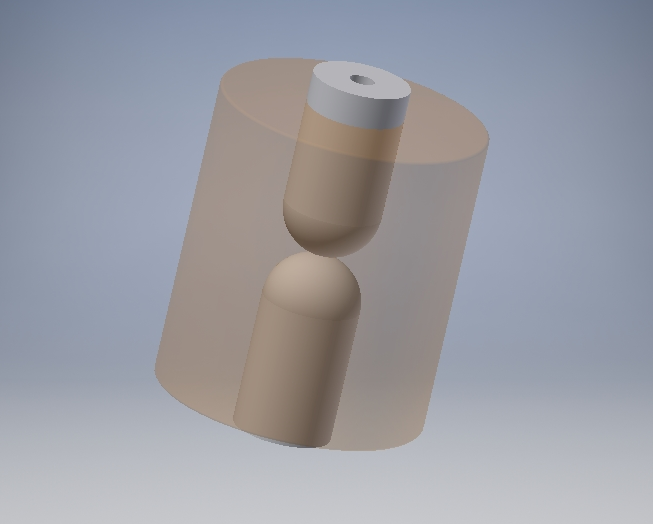
\includegraphics[height=0.2\textheight]{figures/intro/cad_epoxy}}
\caption{CAD model of epoxy specimen used for measurements}
	\label{fig.specimen}
	
	  \end{minipage}
	    \begin{minipage}{0.5\textwidth}
	  
  \centerline{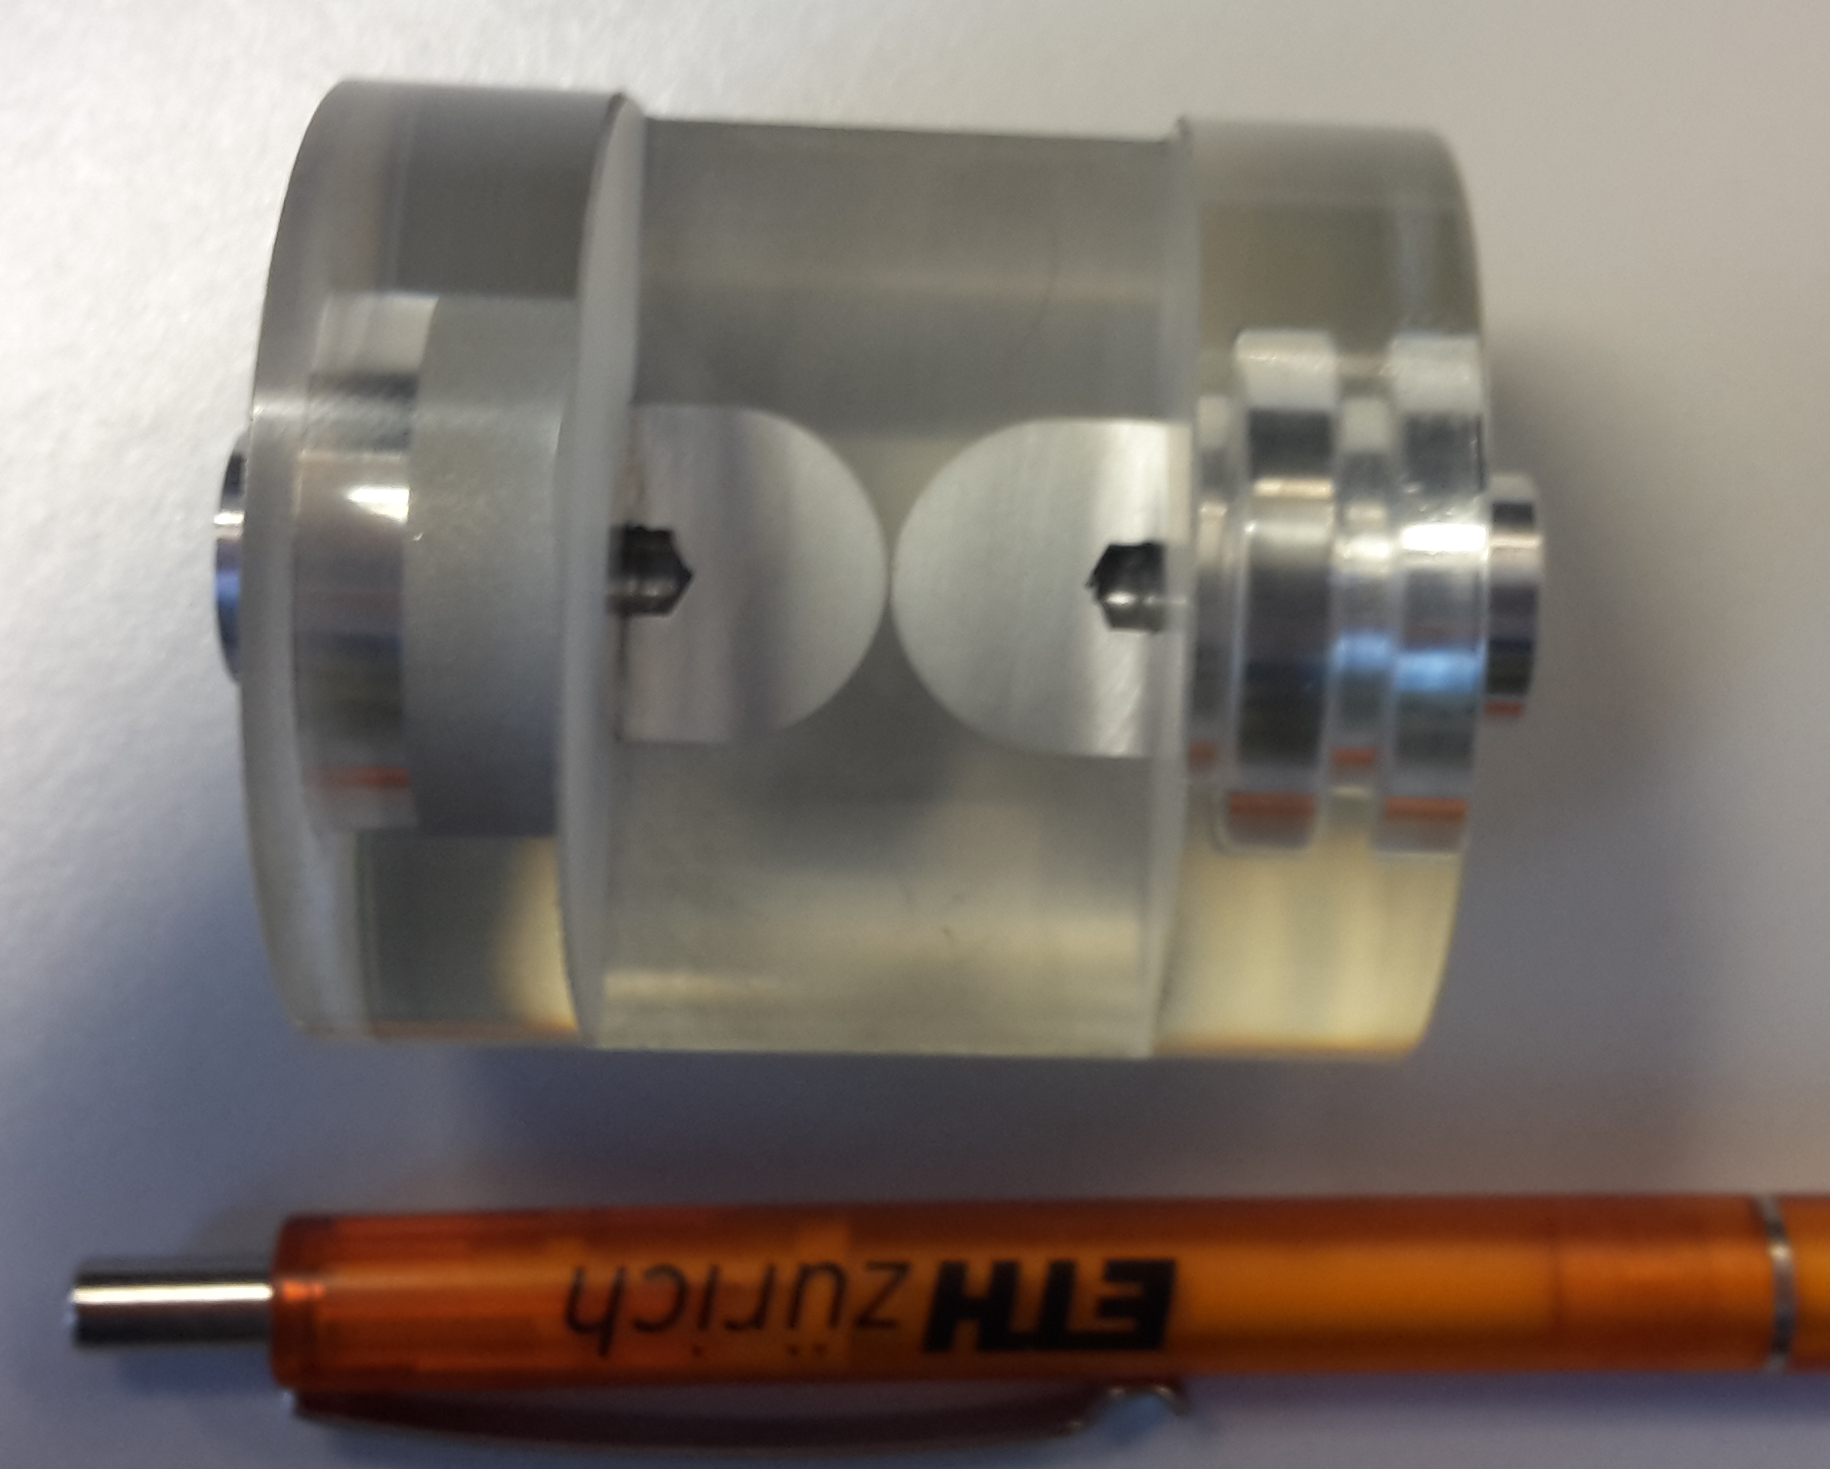
\includegraphics[height=0.2\textheight]{figures/intro/photo_epoxy2}}
\caption{Photo of Epoxy specimen used for measurements of the partial discharges. \protect\footnotemark}
	\label{fig.specimenphoto}
	  
	   \end{minipage}
\end{figure}
\footnotetext{{Both figures provided by Raphael F\"arber}}
In a new approach, a quantification of the pre-breakdown modification within the insulation material should be obtained with the use of an online monitoring of the dielectric permittivity for several harmonics of the applied pulse spectrum \cite{FaerberMVISS}.
The first part of this semester project is aimed at getting the dielectric permittivity by once measuring the capacity of the specimen shown in figure \ref{fig.specimen} in conjuction with numerical field simulations. When using a specimen after manufacturing it is assumed that it's dielectric permittivity is always the same. In order to be able to determine the distance of the two electrodes a reference measurement of the actual distance and the permittivity for two samples is made and a look-up table containing the electrode distance for different vacuum capacities is created. 

The second part of the project is the investigation of the suitability of current transformers in dielectric spectroscopy. With regard to the small capacitive current through the sample, it is the aim to prove or disprove that a current transformer does not deteriorate the signal in a way that makes dielectric spectroscopy is impossible. 



	%
	\chapter{Theory}
\section{Part 1: Determination of electrode distance d}

\subsection{Derivation of the effective dielectric permittivity}
\label{subsec.Derivationeffective}
The effective permittivity $\varepsilon_{\textrm{eff}}$ \nomenclature{$\varepsilon_{\textrm{eff}}$}{effective permittivity} is used to describe the permittivity of a composite material. This is necessary due to the fact that the assumption of homogeneity is not tenable for compound material. As the permittivity is proportional to the capacitance the effective permittivity can be obtained by the ratio of $C^*$ 
\nomenclature{$C^*$}{complex capacitance} to the vacuum capacitance $C_0$.\nomenclature{$C_0$}{vacuum capacitance}

\begin{equation}
\varepsilon_{\textrm{eff}}(\omega) \equiv \frac{C^*(\omega)}{C_0} 
\end{equation}

Whereas the effective permittivity can be derived quite easily from the permittivities of the different materials for layered material geometries this is no more  possible for a complex setup. Thus, a numerical simulation is required as described in chapter \ref{sec.sim_vac_comsol}. In order to get $\varepsilon_{\textrm{eff}}$ the complex capacitance $C^*$ and the vacuum capacitance $C_0$ have to be obtained. While the former can be measured (voltage/current measurement) the latter has to be obtained with a numerical simulation. 
For the specimen in figure \ref{fig.specimen}, there are several geometric quantities that influence the vacuum capacitance. The most important factor is the distance of the electrodes as it may vary considerably. As a consequence, a lookup table has to be created that allows an estimation of d if $C_0$ is given (for details on geometry see section \ref{sec.sim_vac_comsol}). 

 


\subsection{Interdependence between $\varepsilon$ and $\varepsilon_{\textrm{eff}}$} 
$\varepsilon$ is the permittivity of the dielectric. Both $\varepsilon$ and $\varepsilon_{\textrm{eff}}$ are complex figures. Therefore, they can be written as $\varepsilon = |\varepsilon| e^{j \cdot \angle \varepsilon} $ and $\varepsilon_{\textrm{eff}} = |\varepsilon_{\textrm{eff}}| e^{j \cdot \angle \varepsilon_{\textrm{eff}}} $.	
The estimation of the dielectric permittivity of the epoxy in mixed epoxy-air configurations is usually based on the assumption that phase and magnitude of $\varepsilon$ and $\varepsilon_{\textrm{eff}}$ are decoupled. Thus, if one wants to estimate $\varepsilon$ of the dielectric material one has to investigate the dependency of magnitude and phase of the $\varepsilon$ on the $\varepsilon_{\textrm{eff}}$ numerically. This effect can, in general, not be neglected as the simulation for a layered capacitors proves (see figure \ref{fig.layered}).  
\begin{figure}

	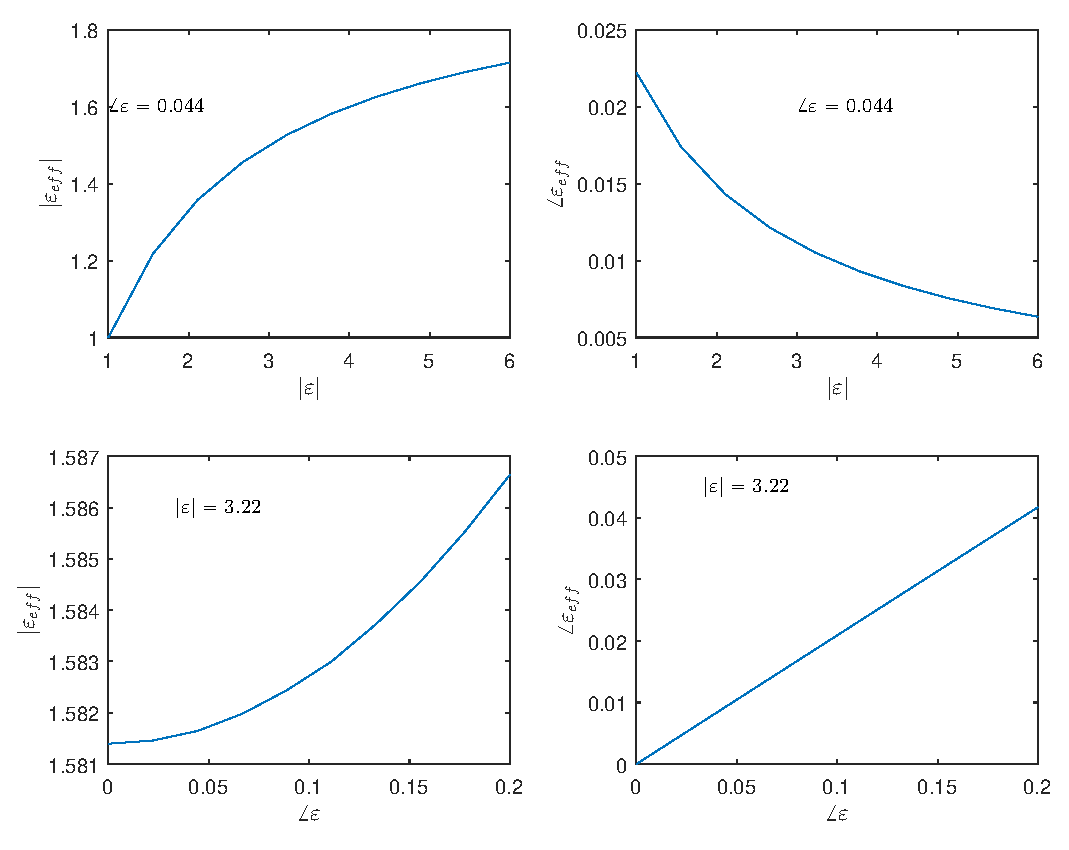
\includegraphics[width=0.8\textwidth]{figures/Theory/layereddielectrics.eps}
	\caption[Kurze Abbildungsbeschreibung]{Interdependeny of permittivity and effective permittivity in phase and magnitude for layered capacitor}
	\label{fig.layered}
\end{figure}
	
	
\section{Part 2: Suitability of current transformer for dielectric spectroscopy}
\subsection{Debye model}
The polarization effects in a dielectric material can be characterized by the (complex) relative permittivity (and the resuling dielectric loss factor). Both are frequency-dependent quantities. 
For linear materials the polarization can be described by a network model. The Debye-ansatz assumes that the rate of change $ \frac{dP_i}{dt}$ is proportional to the difference between the remaining polarization $P_i(t)$  and the polarization at infinity $P_i(\infty$). This results in an exponential relaxation of the polarization function that tends towards $P_i(\infty)$. In an alternating electric field this leads to a phase shift between the electric field $E(t)$ \nomenclature{$E$}{electric field strength} and the  \nomenclature{$D$}{displacement field density}
electric displacement field $D(t)$.\newline
Formally the lagging of the $\underline{D}$ field can be represented by a decomposition in two phasors.
\begin{equation}
 \underline{D}=\epsilon_{0}\epsilon_{r}'\underline{E}-j\epsilon_{0}\epsilon_{r}''\underline{E}
\end{equation}


This exponential decay can be modeled with a \nomenclature{$P_i$}{polarization of material} time constant of a resistor and a capacitor in series ($\tau=R_i \cdot C_i$). Therefore, an emulated dielectric comprises a vacuum capacitance, an additional capacitance $C_i$ and a resistor $R_i$ in series and a resistor $R_{\infty}$ for a stationary conduction current. 


\subsubsection{Derivation of maximum tan($\delta$)}
The aim of this section is to derive the formula for the maximum tan($\delta$) of the Debye model in order to adjust its value to a desired one. The following formula was already stated in \ref{subsec.Derivationeffective}.
\begin{equation}
\varepsilon_{\textrm{eff}} (\omega) = \frac{C^*(\omega)}{C_0}
\end{equation}



In electrical engineering, \nomenclature{$tan(\delta)$}{dielectric loss tangent} it is customary to define the  complex relative permittivity $\varepsilon$ in the following way: 
\begin{equation}
\varepsilon  = \varepsilon_r-j \cdot \varepsilon_r''
\end{equation}
\nomenclature{$\kappa$}{conductivity}
For the delay of the dipole alignment given by the above \nomenclature{$\omega$}{angular velocity} mentioned debye-ansatz, one receives the following equations for the real and imaginary part of $\varepsilon$ \cite{Kuchler}. 
\begin{equation}
\varepsilon'_r = \varepsilon_{\infty} + \frac{\varepsilon_{\textrm{stat}}-\varepsilon_{\infty}}{1+(\omega \cdot \tau )^2}
\end{equation}


\begin{equation}
\varepsilon''_r = \omega \cdot \tau \cdot \frac{\varepsilon_{\textrm{stat}}-\varepsilon_{\infty}}{1+(\omega \cdot \tau )^2}
\end{equation}

The loss tangent \nomenclature{$\varepsilon_{stat}$}{static relative permittivity} is given by:
\begin{equation}
tan (\delta) = \frac{\kappa + \omega \cdot \varepsilon_0 \cdot \varepsilon _r ''}{\omega \cdot \varepsilon_0 \cdot \varepsilon _r '}
\end{equation}
It can be split up in one part for the polarization losses and another part for the conduction losses, which are given in the following equations. 
\begin{equation}
tan (\delta_{L}) = \frac{\kappa}{\omega \cdot \varepsilon_0 \cdot \varepsilon_r'} \newline
\end{equation}

\begin{equation}
tan (\delta_{pol}) = \frac {\varepsilon_r'' } {\varepsilon_r'}
\end{equation}


If measurements are carried out in the frequency domain from $10$ Hz to $10^{7}$ Hz, thus the complex dielectric function can be deduced from a measurement of the  dielectric function $\varepsilon$ as described above. 

\begin{equation}
\varepsilon(\omega) = \frac{1}{j \omega  Z^*(\omega) C_0}
\end{equation}

The impedance of the chosen Debye model is given by 
\begin{equation}
Z_0(\omega)=[\frac{1}{R_\infty}+\frac{1}{R_i+\frac{1}{j \omega C_i}}+j \omega C_0]^{-1} = [\frac{1}{R_\infty}+\frac{j \omega C_i}{j\omega R_i  C_i+1}+j \omega C_0]^{-1}
\end{equation}
Hence,
\begin{equation}
\varepsilon^*(\omega)= \frac{[\frac{1}{R_\infty}+\frac{j \omega C_i}{j\omega C_i R_i  +1}+j \omega C_0]}{j \omega C_0} = \frac{1}{j \omega C_0 R_\infty}+ \frac{C_i/C_0}{j\omega C_i R_i  +1}+1
\end{equation}

The term for $\varepsilon$ is split up into a real and an imaginary part. 

\begin{equation}
\varepsilon_r' = 1+ \frac{C_i/C_0}{\omega^2 C_i^2 R_i^2 +1}
\end{equation}

\begin{equation}
\varepsilon_r'' = -j \left(\frac{1}{\omega C_0 R_\infty}+\frac{\omega C_i^2 R_i / C_0}{\omega^2 C_i^2 R_i^2 +1} \right)
\end{equation}

\begin{equation}
tan(\delta) = tan(\delta_L) + tan( \delta_{Pol}) = \frac{\omega^2 \tau^2+1}{\omega C_0 R_\infty (2+ \omega^2 \tau^2)}+\frac{\omega \tau \Delta \varepsilon}{\varepsilon_{\textrm{stat}} + \omega^2 \tau^2}
\end{equation}

Its derivative is given by: 
\begin{align}
\begin{split}
\frac{\partial tan(\delta)}{ \partial \omega} & = \frac{[\omega C_0 R_\infty (2+\omega^2 \tau^2)]\cdot 2 \omega \tau^2 - (\omega^2 \tau^2 +1) [C_0 R_\infty (2+3 \omega^2 \tau^2)  }{[\omega C_0 R_\infty (2+\omega^2 \tau^2)]^2}\\
					      & + \frac{\tau \Delta \varepsilon [\varepsilon_{\textrm{stat}} + \omega^2 \tau^2] - 2 \omega \tau^2 [\omega \tau \Delta \varepsilon]}{[\varepsilon_{\textrm{stat}} +\omega^2 \tau^2]}
\label{eg:test}
\end{split}
\end{align}
					      
In order to find the maximum of tan($\delta_{pol}$) the first part of the term above, i.e. \eqref{eg:test}, is set equal to 0 to get an algebraic expression for the maximum value and its corresponding frequency. In the following, $\omega_{max}$ refers to the frequency at which $\tan(\delta_{pol})$ is maximum.

\begin{equation}
\tau \Delta \varepsilon [\varepsilon_{\textrm{stat}} + \omega^2 \tau^2] -2\omega \tau^2 [\omega \tau \Delta \varepsilon] = 0
\end{equation}
\begin{equation}
\omega^2 (\tau^3 \Delta \varepsilon -2 \tau^3 \Delta \varepsilon) = - \tau \Delta \varepsilon \cdot \varepsilon_{\textrm{stat}}
\end{equation}
\begin{equation}
\omega_{max}^2 = \frac{\tau \Delta \varepsilon \varepsilon_{\textrm{stat}}}{\tau^3 \Delta \varepsilon}
\end{equation}
\begin{equation}
\omega_{max} = \sqrt{\frac{\varepsilon_{\textrm{stat}}}{\tau^2}}
\end{equation}
\begin{equation}
\tan(\delta_{Pol})_{max} = \frac{\varepsilon_{\textrm{stat}} \Delta\varepsilon}{2\varepsilon_{\textrm{stat}}} = \frac{1}{2} \frac{\Delta \varepsilon}{\sqrt{\varepsilon_{\textrm{stat}}}}
\end{equation}
From here on, $\tan(\delta)$ refers to the pure polarization losses and it is assumed that the conduction losses can be neglected . This is usually the case for polar materials below a certain temperature. 

\section{Fourier Coefficients of trapezoidal pulse  train }

The Fourier coefficients of a trapezoidal pulse train are given by the following equation \cite{FaerberMVISS}. 
\begin{equation}
 U_n = \frac{2 U_0}{j \omega_n T} [e^{\frac{j \omega_n \tau}{2}} \textrm{sinc}{\frac { \omega_n \tau_r }{2}} -e^{\frac{-j \omega_n \tau}{2}} \textrm{sinc}{\frac{ \omega_n \tau_f}{2}}]
\end{equation}
$\tau$ stands for stands for the FWHM (full width half maximum) of one of the trapezoidal pulses.
$\tau_r$ denotes the rise time of the first flank and $\tau_f$ is the fall time of the right flank.

Assume the parameters are as below.
\begin{equation}
\label{eg:taur}
 \tau_r = 0.5e^{-6 } s
  \end{equation}
  \begin{equation}
 \tau_f = 0.1e^{-6} s
  \end{equation}
 \begin{equation}
\tau= 1e^{-6} s
 \end{equation}
 \begin{equation}
 \label{eg:time}
  T=1e^{-3} s
 \end{equation}
 \newpage

The resulting frequency dependency can be seen in  \ref{fig.envelope}

\begin{figure}[H]
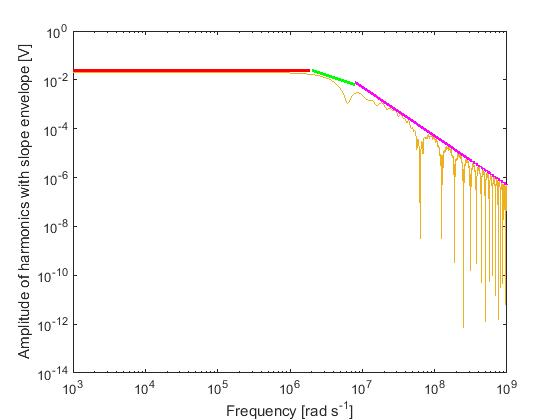
\includegraphics[width=\textwidth]{figures/Method/signal_simulation/envelope.jpg}
\caption[Kurze Abbildungsbeschreibung]{Fourier coefficients of the trapezoidal pulse train with respect to frequency. The solid lines represent the slopes of the envelopes that are caused by the individual 
cutoff frequencies of the parameters defined in \eqref{eg:taur} to \eqref{eg:time}}
\label{fig.envelope}
\end{figure}

Slopes of the curves: \newline
\begin{itemize}
 \item 0 on loglog plot for $\omega < \frac{2}{\tau}$\newline
\item -20dB/decade on loglog plot after $\omega = \frac{2}{\tau}$ \newline
\item -40dB/decade on loglog plot after $\omega = \frac{2}{\tau_r}$\newline

\end{itemize}




	
\subsection{Devices for high frequency current measurement}
The most common method for high frequency current measurement from DC up to the GHz region are shunt resistors. They make use of the the proportionality between the current and a voltage drop over the shunt. Besides, they are passive and have high bandwidths up to the GHz region. Another advantage is their ability to monitor DC currents. In order to keep the reduction of the current rate of rise in an acceptable range the self-inductance is often kept low by using coaxial shunts. \cite{highdynamiccurrent}
A current transformer (CT) or pulse transformer is an instrument transformer that creates an AC-voltage on its secondary side that is proportional to the alternating current on its primary side. Most common are toroidal cores that are coiled. The secondary side has a low output resistor (usually 50 $\Omega$).
The principle setup of a current transformer is shown in the following figure: 
\\CTs are as well suitable if the current on the primary side is too high to measure because the CT provides a voltage on the secondary side that is in a measurable area. A current transformer is suitable for current amplitudes from microamperes to megaamperes. A further advantage over a shunt resistance represents the galvanic isolation of the secondary side from the primary. This galvanic isolation prohibits large voltages on the secondary side (at measuring inputs) which might destroy the Butterworth-Filter or the Analog-to-Digital-Converter (ADC). \nomenclature{$\textrm{ADC}$}{Analog-to-Digital converter}
The transfer function for the current transformer can be calculated with the following differential equation, that is derived from Ampere's law (derivation based on: \cite{highdynamiccurrent}).\\
\begin{figure}
	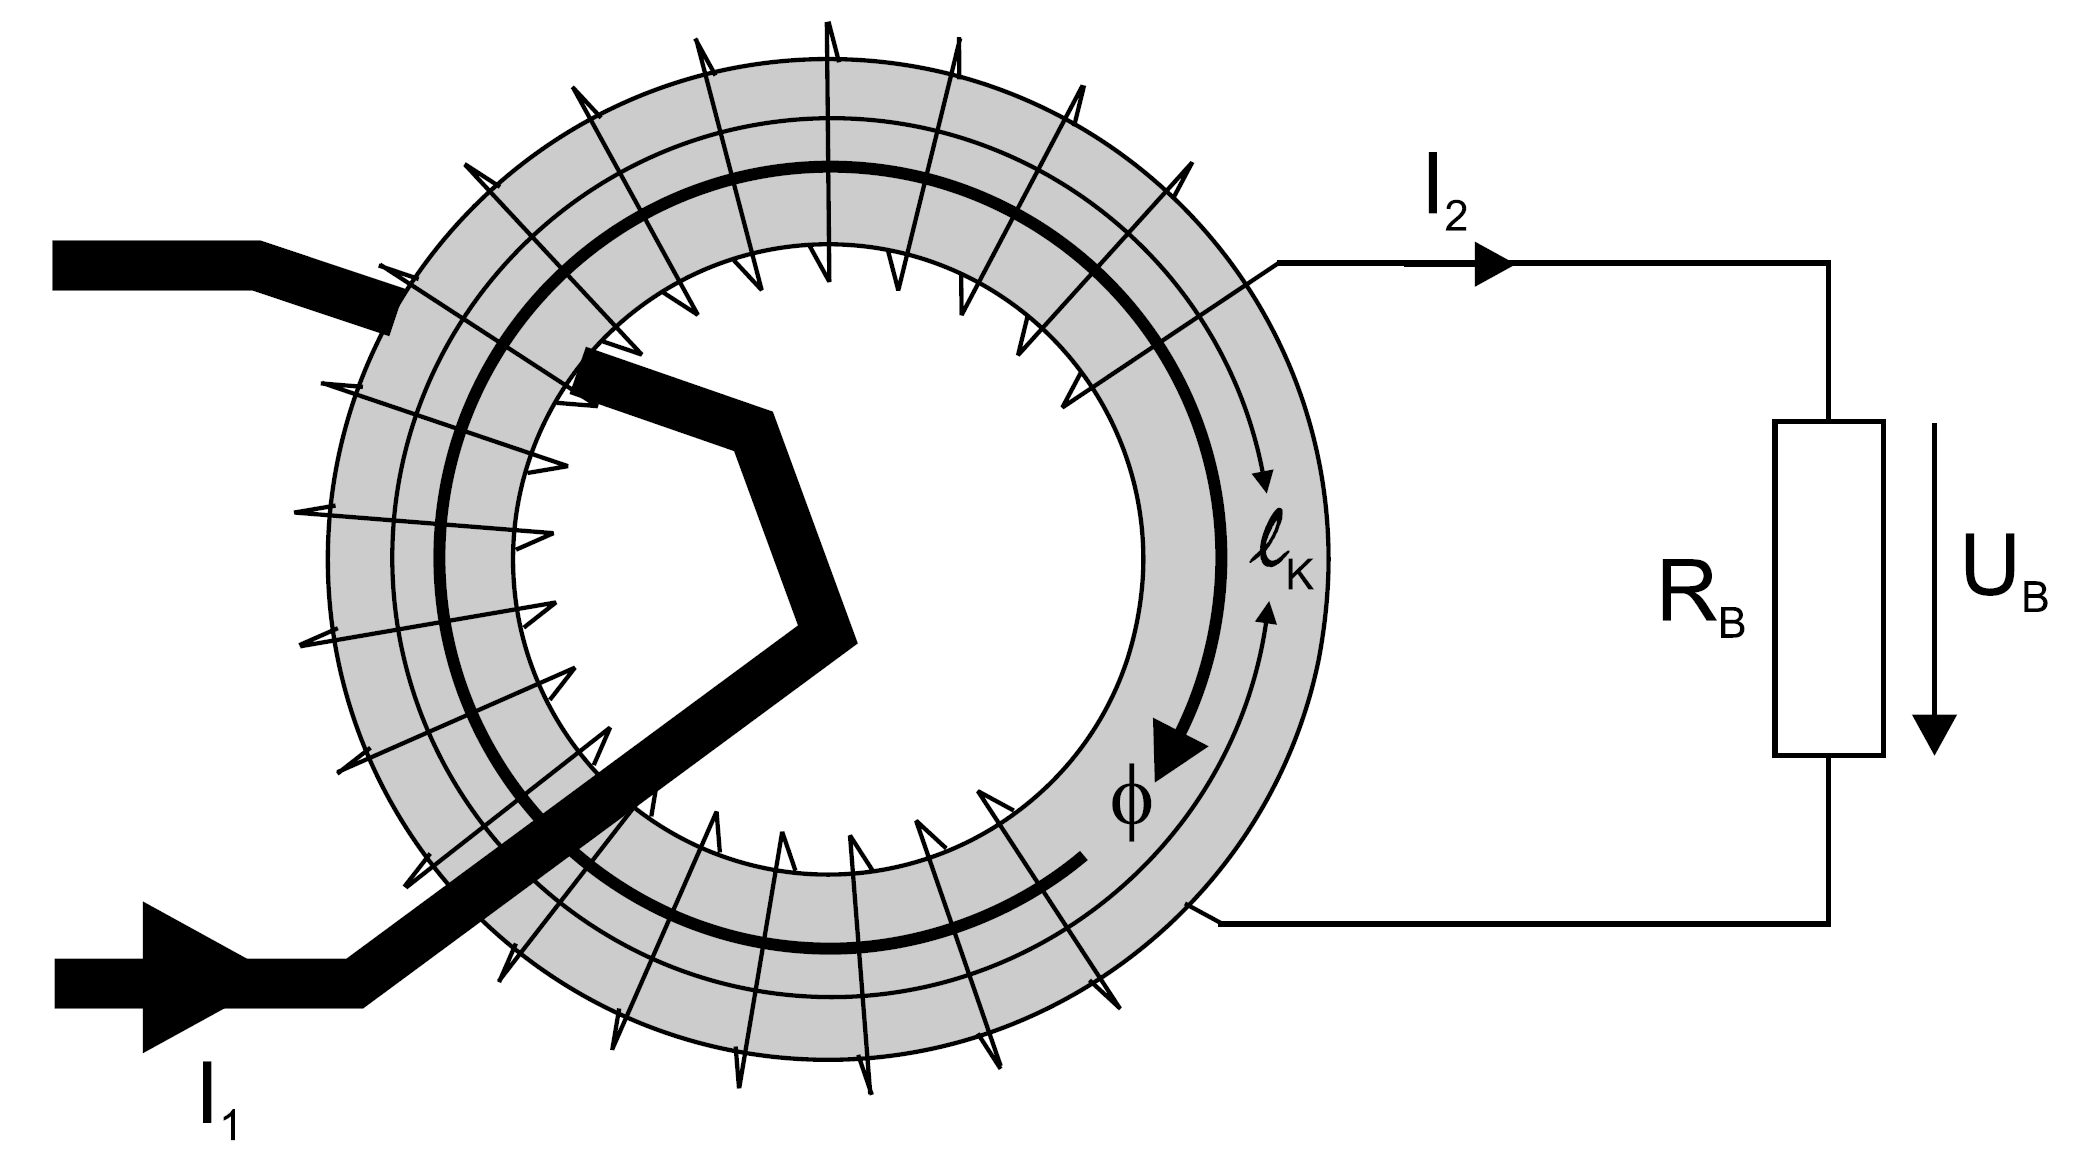
\includegraphics[width=0.8\textwidth]{figures/Theory/ct_setup}
	\caption[Kurze Abbildungsbeschreibung]{Structure of a current transformer with a primary current, a ring core and a secondary winding \protect\footnotemark}
	\label{fig.ct_setup}
\end{figure}
\footnotetext{figure taken from \cite{highdynamiccurrent}}

\begin{equation}
U_B(t) + \frac{L_2}{R_B} \cdot \frac{dU_B(t)}{dt}=\frac{N_1}{N_2} \cdot L_2 \cdot \frac{dI_1(t)}{dt}
\end{equation}
This results in a complex transfer function of: 
\begin{equation}
U_B(s) = R_B \cdot \frac{N_1}{N_2} \cdot \frac{s \frac{L_2}{R_B}}{s \frac{L_2}{R_B} +1} \cdot I_1(s)
\end{equation}

With the time constant $T=\frac{L_2}{R_B}$ this is a high-pass filter with a lower corner frequency of 
\begin{equation}
f_u= \frac{1}{2 \pi T} = \frac{R_B}{2 \pi L_2}
\end{equation}

For frequencies above the corner frequency the transfer function is:
\begin{equation}
G_CT(s) = \frac{U_B(s)}{I_1(s)}=R_B \cdot \frac{N_1}{N_2}
\end{equation}

This simplified model ignores the resistance and inductance of the primary and secondary side. 
For simplicity reasons the transfer function of a current transformer was assumed to be constant for the measurement, but this neglects the resistance and inductance of the primary and secondary side. Although this transfer function can only be used within a certain frequency range (in our case 300 Hz...300 MHz) errors introduced by this simplication have to be considered. 


\subsection{Noise Considerations}
\subsubsection{General}
The evaluation of noise added to the signal by the CT, the integrator, the BW-filter and the cables is of great importance as it limits the capability of resolving small values of tan($\delta$).
In order to quantify the desired signal compared to the background noise, the Signal-to-Noise Ratio (SNR) \nomenclature{$\textrm{SNR}$}{Signal-to-Noise-Ratio} can be measured. SNR is  the ratio of signal power over noise power. The power is proportional to the amplitude of the signal, hence \nomenclature{$\textrm{NF}$}{noise figure}
\begin{equation}
	\textrm{SNR}=\frac{P_{\textrm{signal}}}{P_{\textrm{noise}}} = \left[\frac{V_{\textrm{signal}}}{V_{\textrm{noise}}^{\textrm{rms}}}\right]^2
\end{equation}
The degradation of the SNR is characterized by its input value over its output value, which is the Noise Figure (NF) and is indicated in dB.
\begin{equation}
	\textrm{NF} = 10\cdot \log\left(\frac{SNR_{\textrm{in}}}{SNR_{\textrm{out}}}\right)
\end{equation}
Thus, the amount of noise added by the components can be characterized by the NF. 



	%
	\chapter{Methods}
\section{Part 1}
\subsection{General approach}


The setup is illustrated in figure \ref{sec.setup_amp_1} . The expoid resin specimen is put into a cell. The DLPCA amplifier converts the measured current into a voltage and after a butterworth filter an ADC creates a signal that is processed with MATLAB. 

\begin{figure}[htbp]
	\centering
	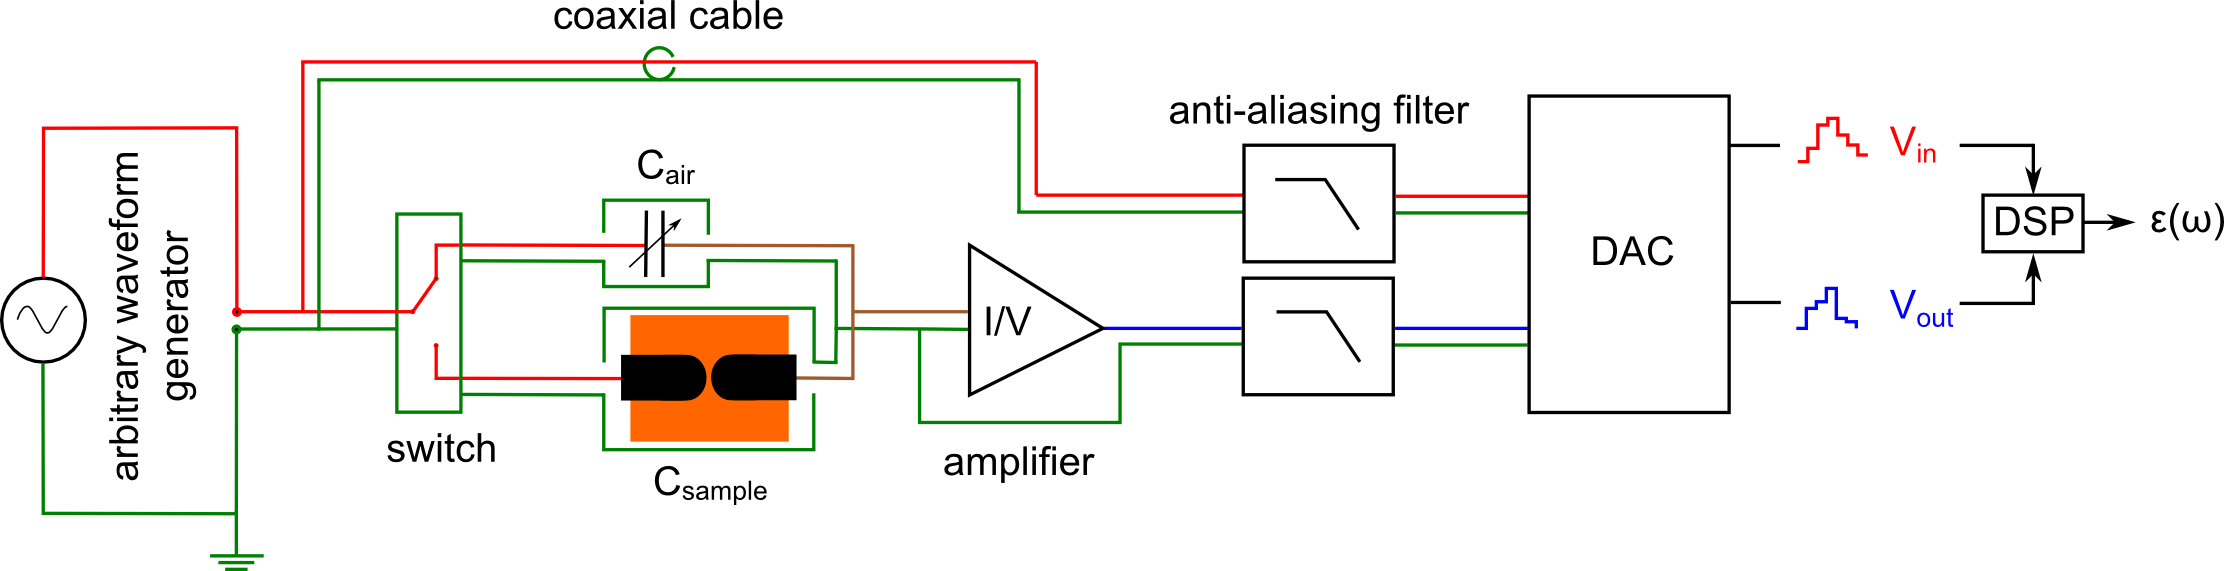
\includegraphics{figures/Method/setup/setup_amplifier.png}		
	\caption[Kurze Abbildungsbeschreibung]{Setup for measurements\footnote{source: Raphael F\"arber}} 
	\label{sec.setup_amp_1}

\end{figure}
\label{sec:general_approach}
The following method is based on the assumption that  the epsilon is always the same for the used samples when they are delivered. Thus, there is just a need to determine the distance of the electrodes for each delivered sample in order to be able to calculate the effective $\epsilon$ after below-PD current measurements, because the distance might vary considerably. 
At first the initial $\epsilon_eff$ for two reference samples has to be obtained:\\
For the two reference samples the distance is measured optically with a microscope. By using the $d-C_0$ look up table described in the following chapter the vacuum capacitance can be obtained from the optical distance measurement. Together with the measured capacitance $C*$ a guess of the effective epsilon for the used epoxy resin is possible. 

For forther samples, the capacitance $C*$ has to be measured. Together with the initial value of $\epsilon_eff$ of the reference samples one can obtain the vacuum capacitance $C_0$.By using the $d-C_0$ look up table a guess of the electrode distance d is possible. Now, the vacuum capacitance and the corresponding electrode distance are known for further measurements. Thus, it is possible to get the effective 
\subsection{Simulation of vacuum capacitance} 
As mentioned in the chapters before the vacuum capacitance cannot the calculated directly because of the complexity of the geometry. COMSOL is a simulation software that is suitable for a numerical estimation of a permittivities or capacitances. The dependency of the vacuum capacity $C_0$ has to be simulated numerically both for the high-voltage setup and for the low-voltage setup. Although all measurements and the corresponding calculations of section \ref{sec:general_approach} can be carried out in the low-voltage setup it is handy to be able to do these calculations in the high-voltage setup as well. 

\begin{figure}[htbp]
	\centering
	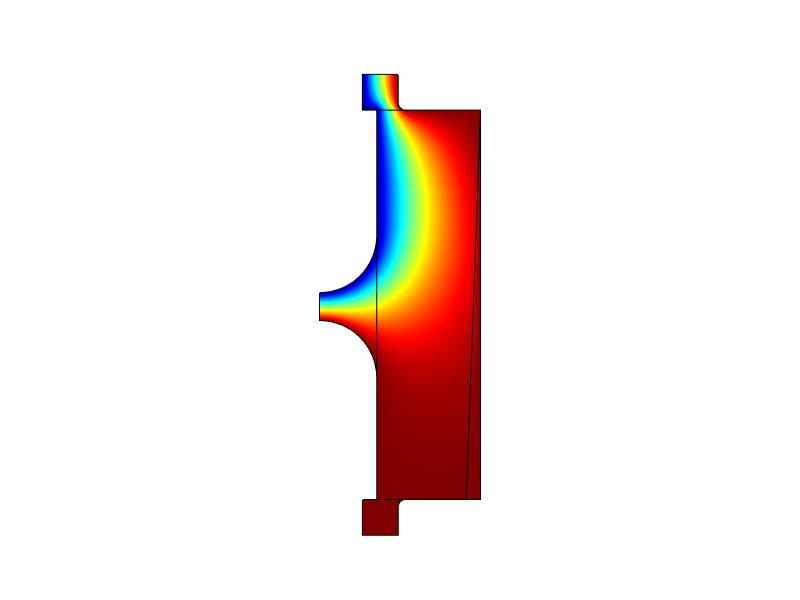
\includegraphics{figures/COMSOL_Beispielbild.jpg}		
	\caption[Kurze Abbildungsbeschreibung]{Field simulation of the low-voltage test cell (0.5 mm electrode distance)} \ref{sec.analysecurrent}
	\label{fig.waveforms}
\end{figure}
 
There are several systematic errors that influence the vacuum capacity simulation. One factor is the air gap between the wall of the low-voltage setup and the specimen. This air gap is unavoidable in order to be able to remove the specimen from the pouring setup. This air gap should theoretically be 0.5 mm, but in practice it is expected to vary between 0 mm and 1 mm for the worst-case. The lookup table of d based on $C_0$ is based on an air gap of 0.5 mm, therefore the deviation from this value has to be investigated numerically.
Another systematic error is the deviation of the height of the specimen. During  the pouring process the height of the specimen cannot be fixed precisely. The maximum deviation is expected to be $\pm$ 0.5 mm. This deviation might occur during the production process of each new specimen. Thus, if the electrode distance of a specimen should be estimated by the method described in !!! 

\section{Part 2}
\subsection{The setup}
There are two general setups. One is the high-voltage setup and one the low voltage-setup. For testing the suitibility of the current transformer the low voltage setup is sufficient. This is reached with a 1000 times higher vacuum capacitance in the Debye model which guarantees that the current is the same as in the high voltage setup with a voltage that is 1000 times higher. 

The following graph \ref{sec.setup_amplifier} illustrates the setup for measurements without a current transformer. The DLPCA-200 is a variable gain low noise current amplifier that has a transimpedance gain from $10^3$ to $10^11 V/A$. MATLAB automatically adapts its gain to a value that is suitable for the input voltage area of $\pm 10V$. 

\begin{figure}[htbp]
	\centering
	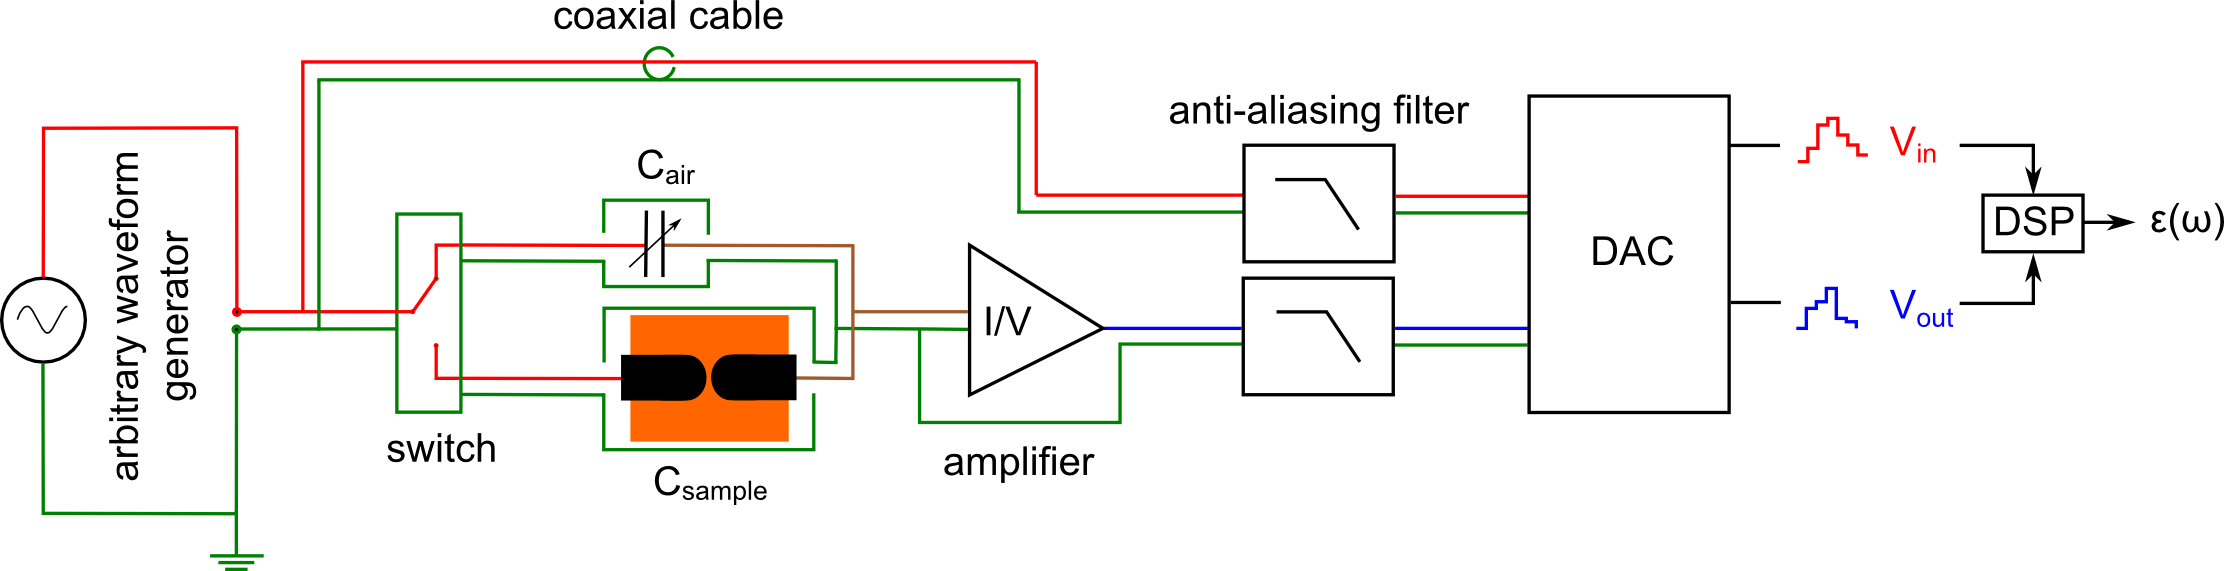
\includegraphics{figures/Method/setup/setup_amplifier}		
	\caption[Kurze Abbildungsbeschreibung]{Setup for reference measurements {source: Raphael F\"arber, revised by authors}} 
	\label{sec.setup_amplifier}

\end{figure}

Afterwards, the DLPCA is replaced with a current transformer. 
\begin{figure}[htbp]
	\centering
	\includegraphics{figures/Method/setup/setup_CTonly}		
	\caption[Kurze Abbildungsbeschreibung]{Setup for measurements with Current Transformer only {source: Raphael F\"arber, revised by authors}} 
	\label{sec.setup }

\end{figure}


\section{Signal analysis of the Debye model}

In order to emulate different dielectrica with their own respective dielectric loss tangent, different combinations of circuit elements were used. Each different circuit accounts for another loss tangent with respect to frequency. With the objective to assess the performance of the current transformer, reasonably high values for the $tan\left(\delta\right)$ were assumed (i.e. 0.05 to 0.2) since a lower loss tangent would require a higher resolution on the part of the current measurement.


\begin{figure}[htbp]
	\centering
	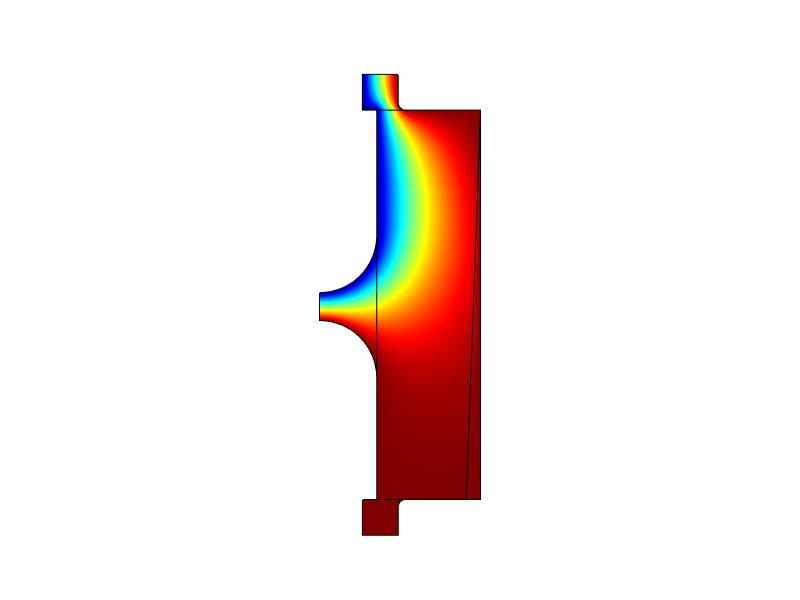
\includegraphics{figures/COMSOL_Beispielbild.jpg}		
	\caption[Kurze Abbildungsbeschreibung]{Electron drift currents in Ar at 30 Td and in CO$_2$ at 65 Td, the latter was divided by 10 and shifted by 0.2 $\mu$s. Dotted lines are averages of measured waveforms, solid lines are fits of Eq. XX. $T$ marks the electron transit time, and the markers $T_1$ to $T_3$ are explained in section.} \ref{sec.COMSOL_Beispielbild}
	\label{fig.waveforms}
\end{figure}


\subsection{Design of a holder for the Debye Equivalent Circuit}
For a lossy medium the Debye Network consists at least of a vacuum capacity $C_0$ and the term for the charging of the additional capacitance. There might be . Thus, it is reasonable to design a holder for the network that can hold three strands with two components each. Moreover, it has to fit into the low-voltage and high-voltage test cell. 

\begin{figure}
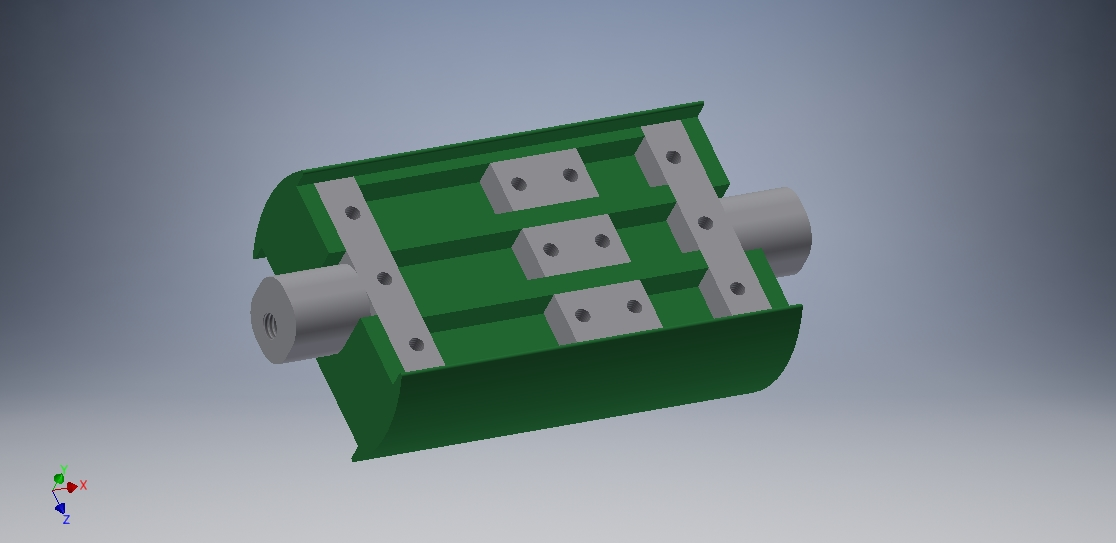
\includegraphics[width=\textwidth]{figures/Method/CAD_MODEL/Gesamtanordnung.jpg}
\end{figure}
\newpage

\begin{sidewaysfigure}
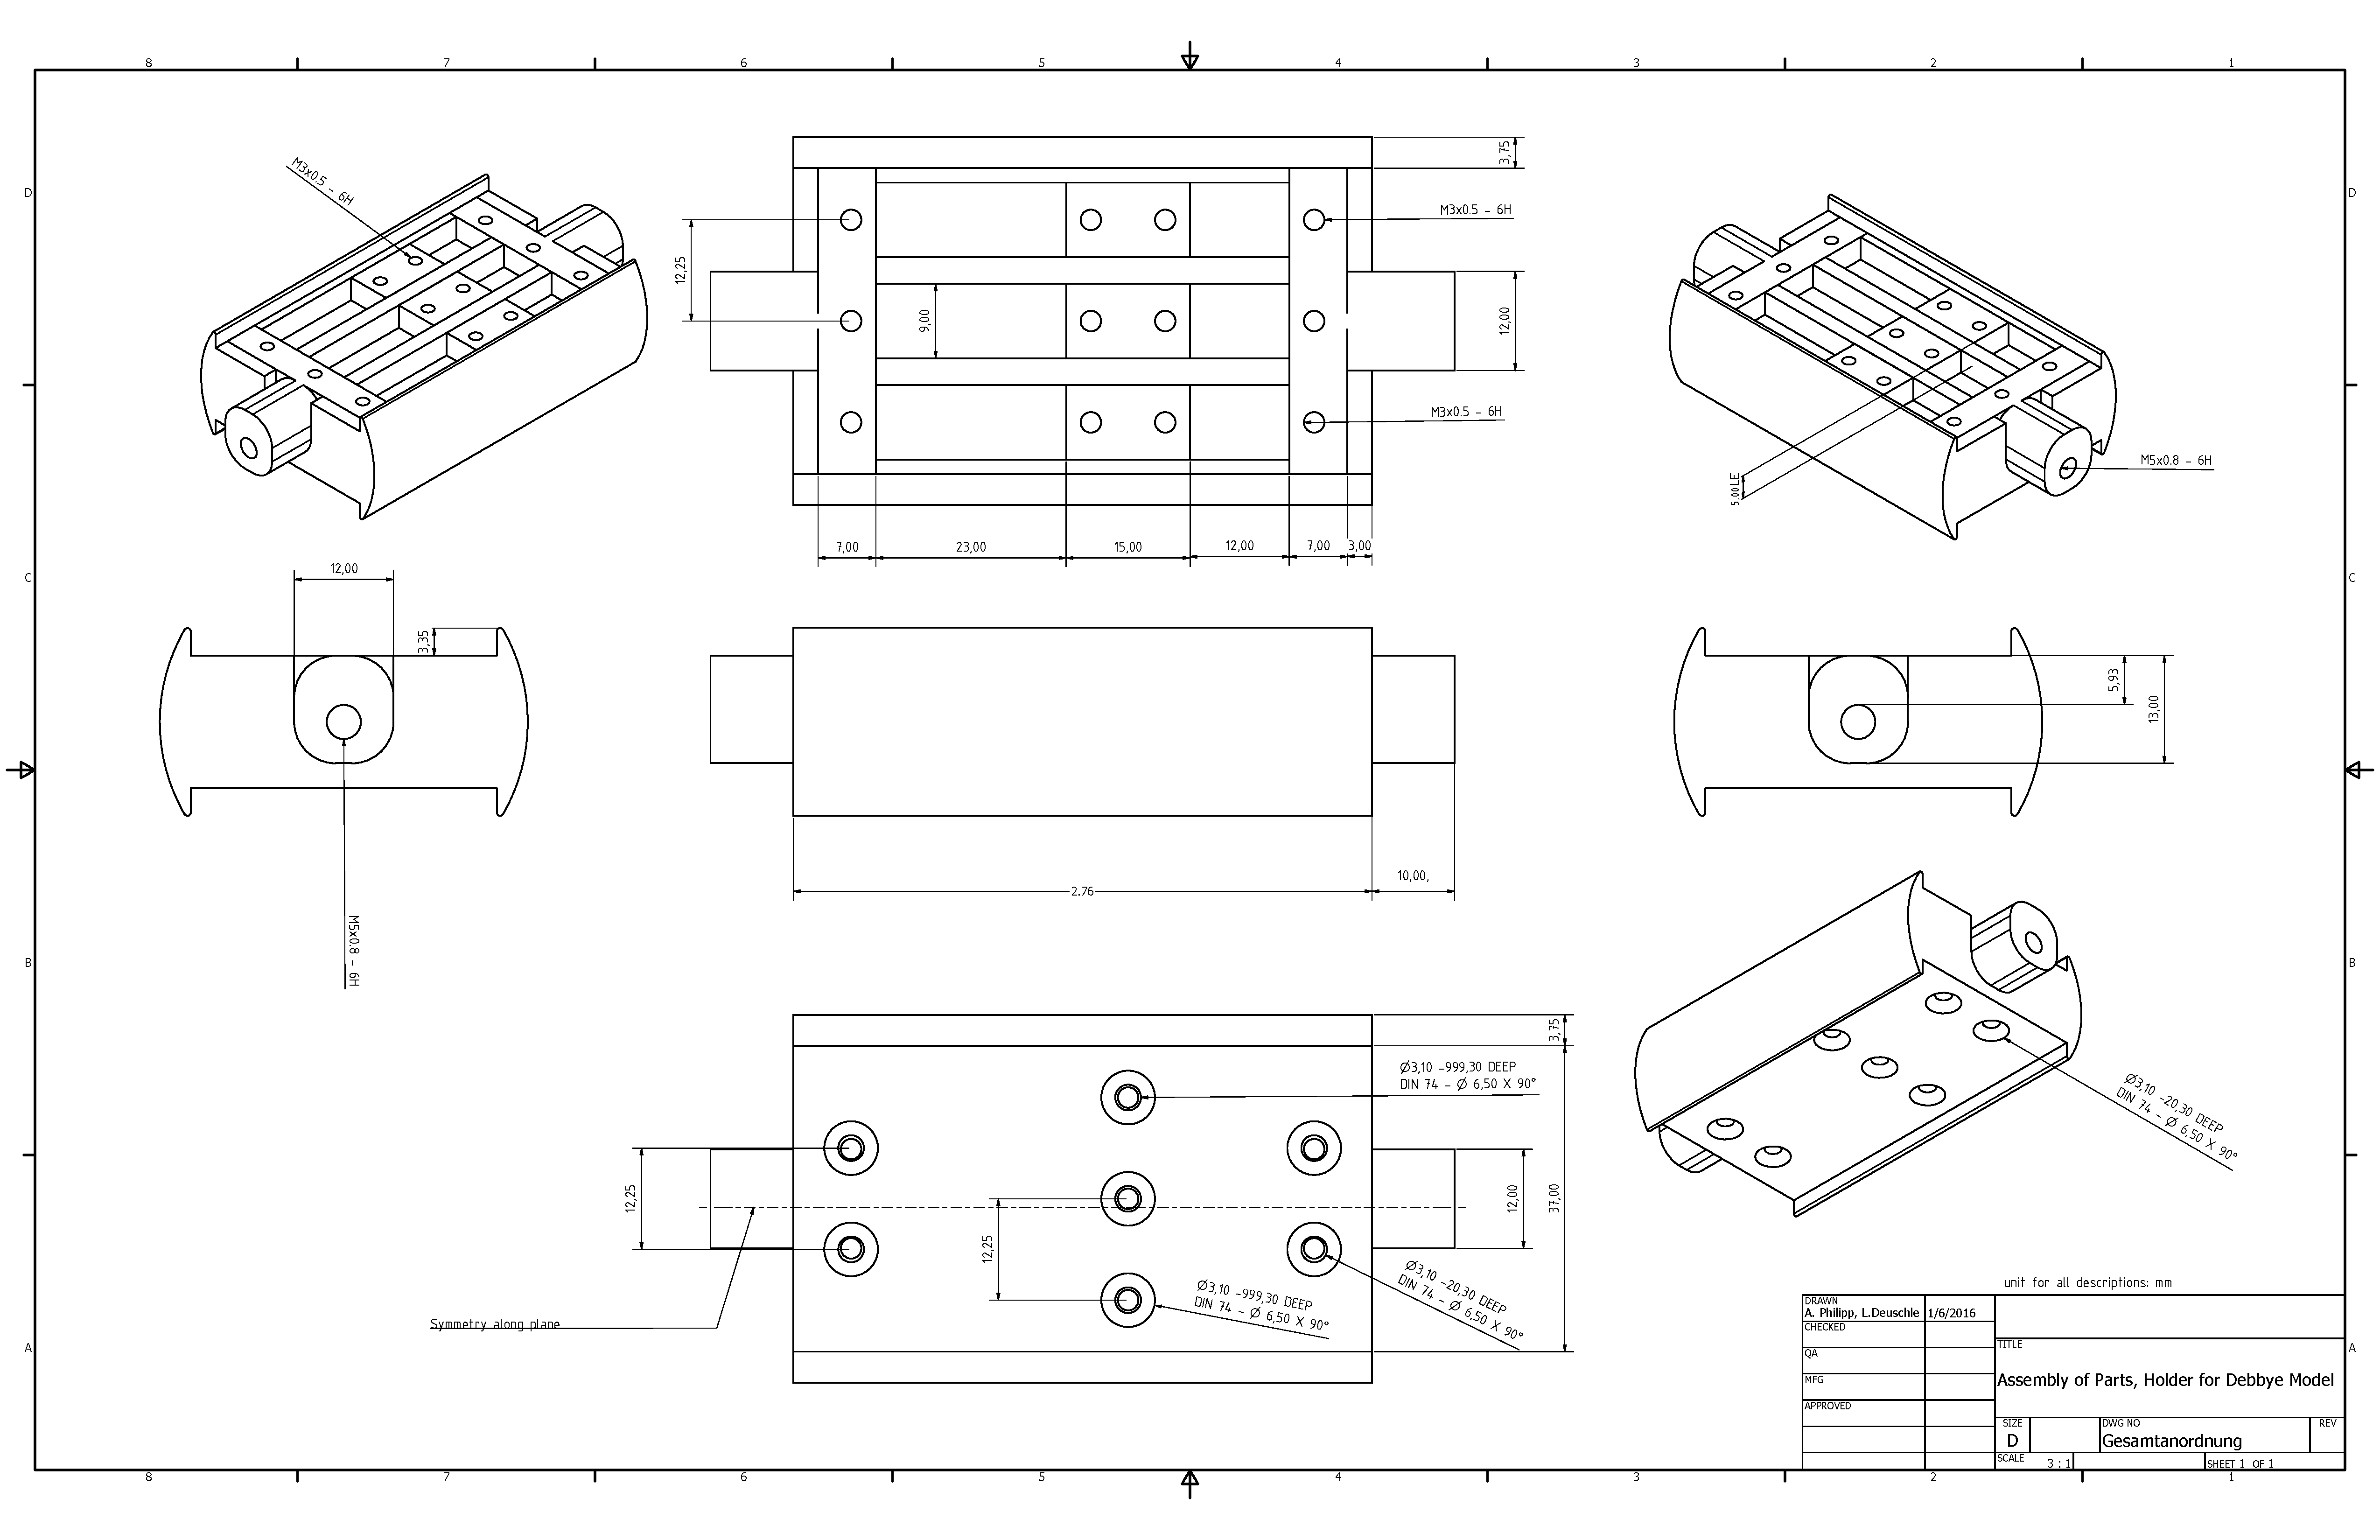
\includegraphics[width=0.99\textwidth]{figures/Gesamtanordnung.pdf}
    \caption{Property profile of the diverse library compared to the compound pool.}
    
   \end{sidewaysfigure}	
\newpage
    

\subsection{Measurement of the textepsilon and the tan(textdelta) for the Debye model}

The aim is to have a current flwoing though the Debye model in the low-voltage setup that is oft the same order as a current in the high voltage-setup. In order to have a comparable current for a voltage that is $1/1000$ of the high-voltage setup a capacitance $C_0$ for the Debye is selected 1000 times higher than the Capacitance of the samples. As the sample has a capacitance of 3.44 pF its equivalent $C_0$ in the debye-model is 3.3 nF. In order to get a tan($\delta$) of !!! $R_i$ is chosen as and $C_i$ is chosen as .
\begin{figure}
	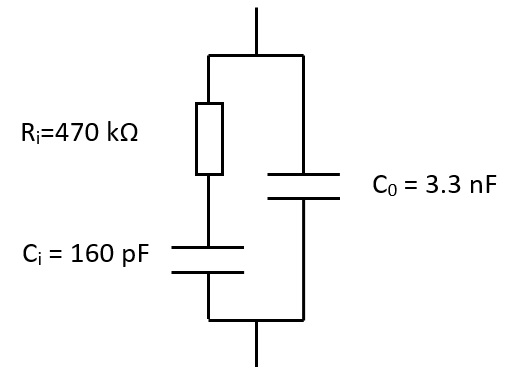
\includegraphics{figures/Method/debye-modell.jpg}	
	\caption{Debye model for tan($tan(\delta)$)= }	
\end{figure}






\subsection{Integrator}
\subsection{Advantages of using an integrator}
As the used 16-bit DAC has a limited resolution it is advantageous to use an integrator in order to spread the frequencies of the signal over a larger timescale. This makes it possible to detect the different frequencies more accurately with the same DAC. 
A second reason to make use of an integrator is due to the fact that it adds an additional factor of $1/f$ to the Fourier spectrum of the output voltage signal. As the Fourier spectrum of the input signal is as well characterized by a $1/f$ decrease the integrator transforms the pulse signal back to a trapezoidal signal with a $1/f$-dependency in the Fourier spectrum. Since a $1/f$ dependency in the output signal is preferable to a constant Fourier spectrum due to better resolution for the first harmonic, the integrator improves the measurement as well. 
\subsection{Design of integrator}
The integrator should have two functions. On the hand side it should integrate signal on the other hand it should amplify the signal by a factor of 1000. This is due to the fact small below-PD-currents ($\sim$mA) should be measured. With a CT-sensitivity of $1V/A$ an amplification of 1000 is reasonable to use the range of measurable inputs of $\pm$ 10 V. These requirements can be achieved by a non-inverting integrator, which is shown in figure  \ref{fig.circuit}. 

\begin{figure}
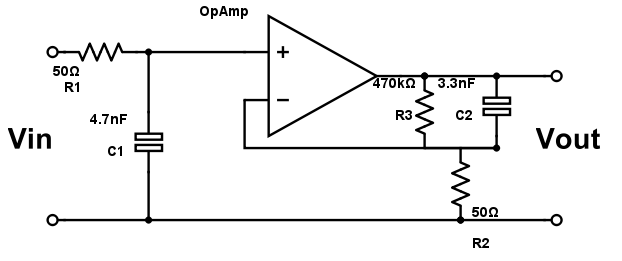
\includegraphics[width=0.99\textwidth]{figures/Method/integrator/circuit.png}
    \caption{Property profile of the diverse library compared to the compound pool.}
    \label{fig.circuit}
    \end{figure}	


The integrator has the following transfer function: \\
\begin{equation}
	tf_int(j \omega)=1/(1+s R_1 C_1)*(1+(1/R_2)*(1/R_3+j \omega C_2)^-1)
\end{equation}
The transfer function of the integrator is illustrated by the following bode plot. 

\begin{figure}

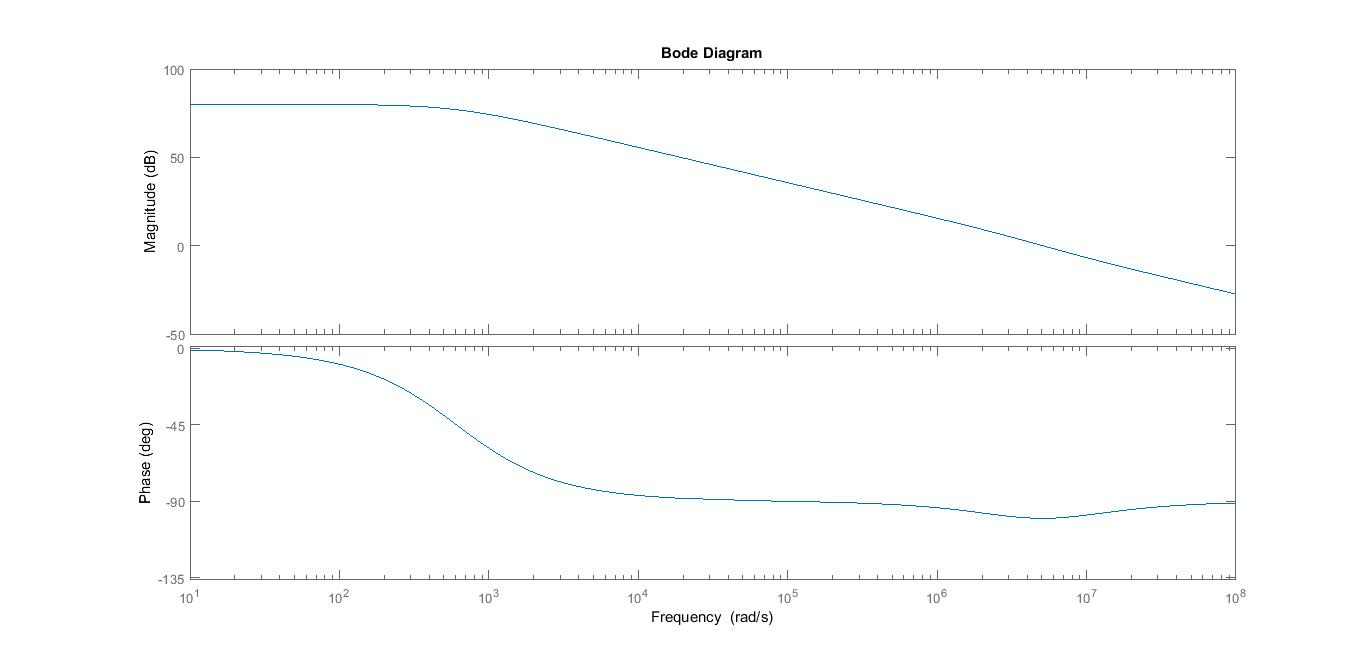
\includegraphics[width=\textwidth]{figures/Method/integrator/transferfunction_int.jpg}

\caption[Kurze Abbildungsbeschreibung]{Bode plot of an integrator } \ref{sec.Bodeplot}
\end{figure}

\begin{sidewaysfigure}
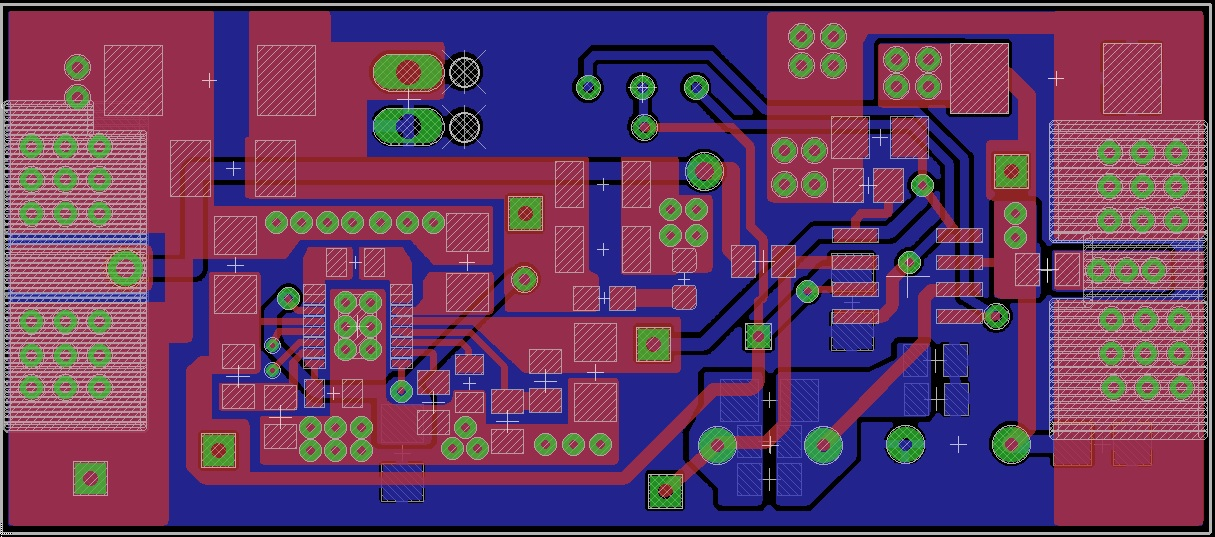
\includegraphics[width=0.99\textwidth]{figures/Method/integrator/PCB_Integrator.png}
    \caption{Printed Circuit Board Layout for the non-inverting ingrator with a DC voltage supply}
    
    \end{sidewaysfigure}	
    
    
    \newpage
    
    	\begin{sidewaysfigure}
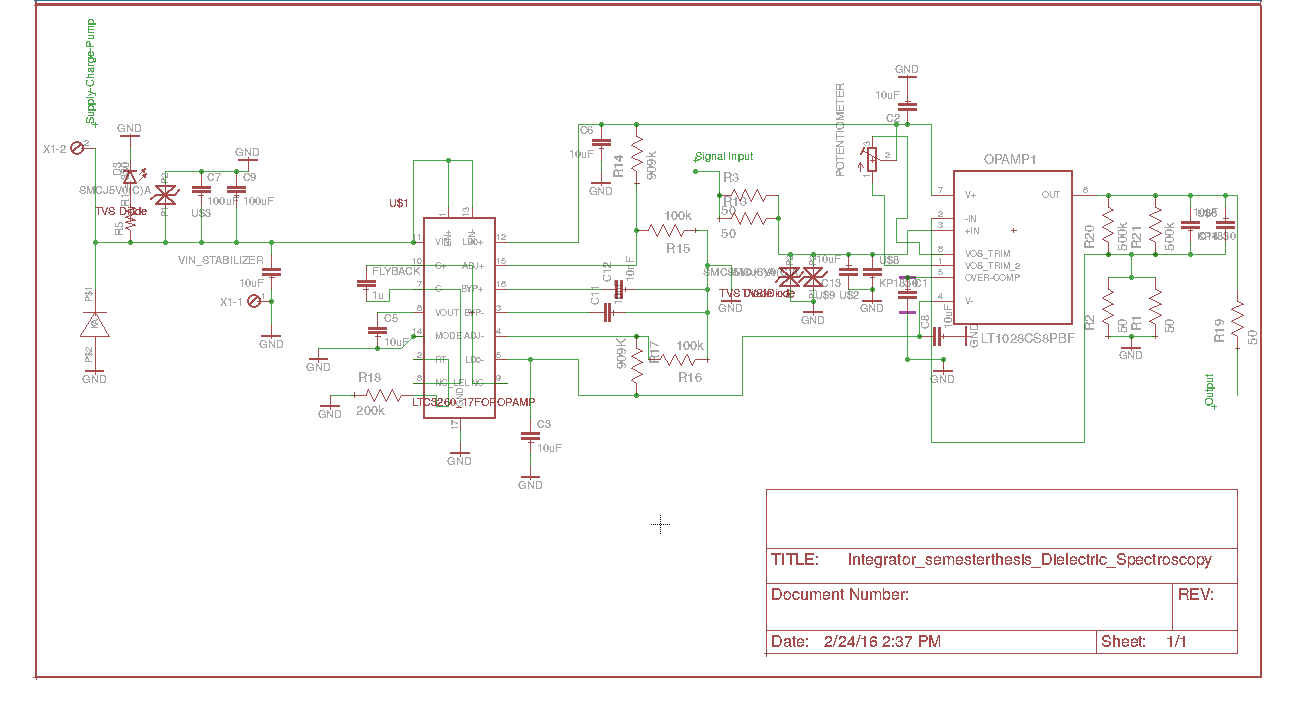
\includegraphics[width=0.99\textwidth]{figures/Method/integrator/schematic.jpg}
 \caption{Property profile of the diverse library compared to the compound pool.}
  \end{sidewaysfigure}	

	



\subsection{Protective Clamping Capability of the current transformer}


	%
	
\chapter{Results}
\section{Simulation of Capacitance values}
\subsection{Comparision of Capacitance in the simulation with a sphere geometry}
The simulation of the capacitance for the cylindric geometry as a function of different distances with COMSOL leads to the following figure.The simulation of two spheres as well as the approximation formula result in a general 
shift which is due to the fact that it is a three electrode arrangement as the wall of the
low-voltage introduces a new capacitance between the upper electrode and the wall which is not affected by the distance variation. This results in a reduction of the capacitance compared to the 
two spheres geometry. Thus, the simulated values for the low voltage test cell seem reasonable if one compares them to the results of the capacitance between two spheres. \newline 

\begin{figure}[htbp]
	\centering
	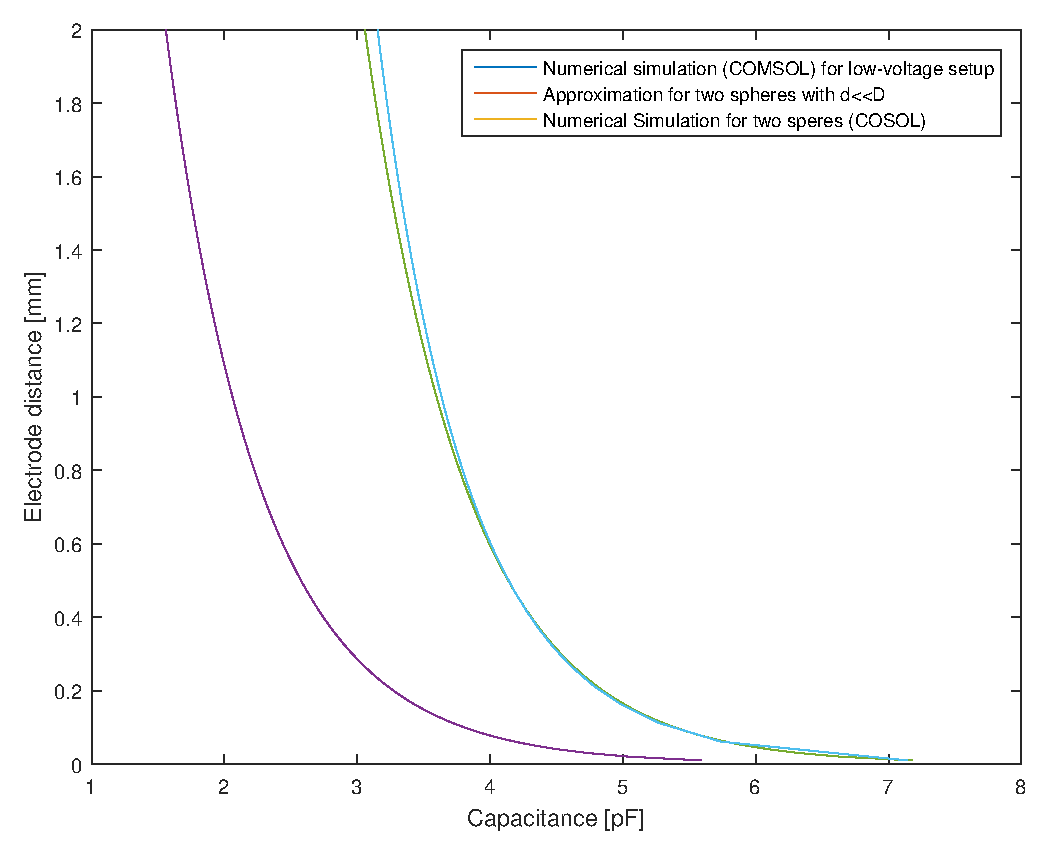
\includegraphics[scale=0.3]{figures/Method/Part1_d_C0/Comparison_Low_voltage_Two_spheres.eps}		
	\caption[Kurze Abbildungsbeschreibung]{Dependency of the electrode distance on the capacitance for the low voltage setup and two spheres $\epsilon = 3.5$ } 
	\label{fig.waveforms}
\end{figure}

\subsection{Complex effective permittivity}
As it was mentioned in the theory chapter, generally speaking, magnitude and phase of the effective permittivity in relation to the
real permittivity of the dielectric are not decoupled quantities. While this effect becomes especially apparent in horizontally layered dielectrics for a
a capacitance with horizontal parallel plates, the graphs below show that the effect for the specimen in the low-voltage cell are negligible. That means a purposely exaggerated variance for both parameters
results in a change in the other parameter that is below 0.1\%.

\begin{figure}[htbp]
	\centering
	\centerline{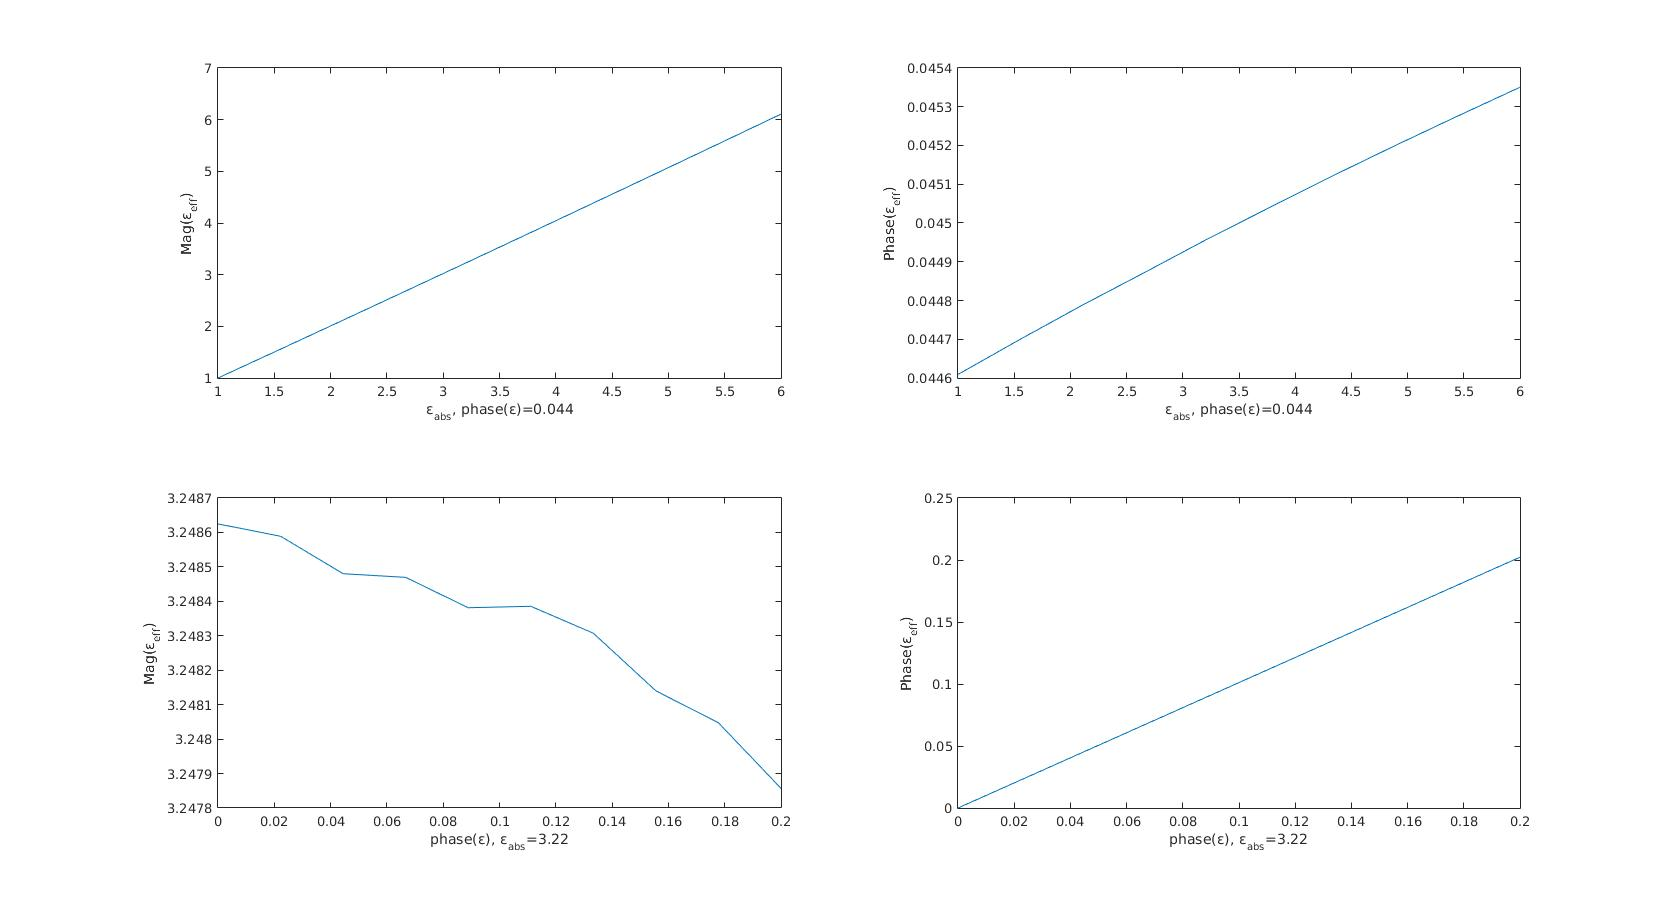
\includegraphics[width=0.5\textwidth]{figures/Results/Complex/complex_permittivity_specimen}}		
	\caption[Kurze Abbildungsbeschreibung]{Interdepedency of phase and magnitude of the effective permittivity (airgap=0.5mm) } 
	\label{fig.complex}
\end{figure}

\section{Capacitance of specimen and effective permittivity}
\begin{figure}[ht]
	\centering
	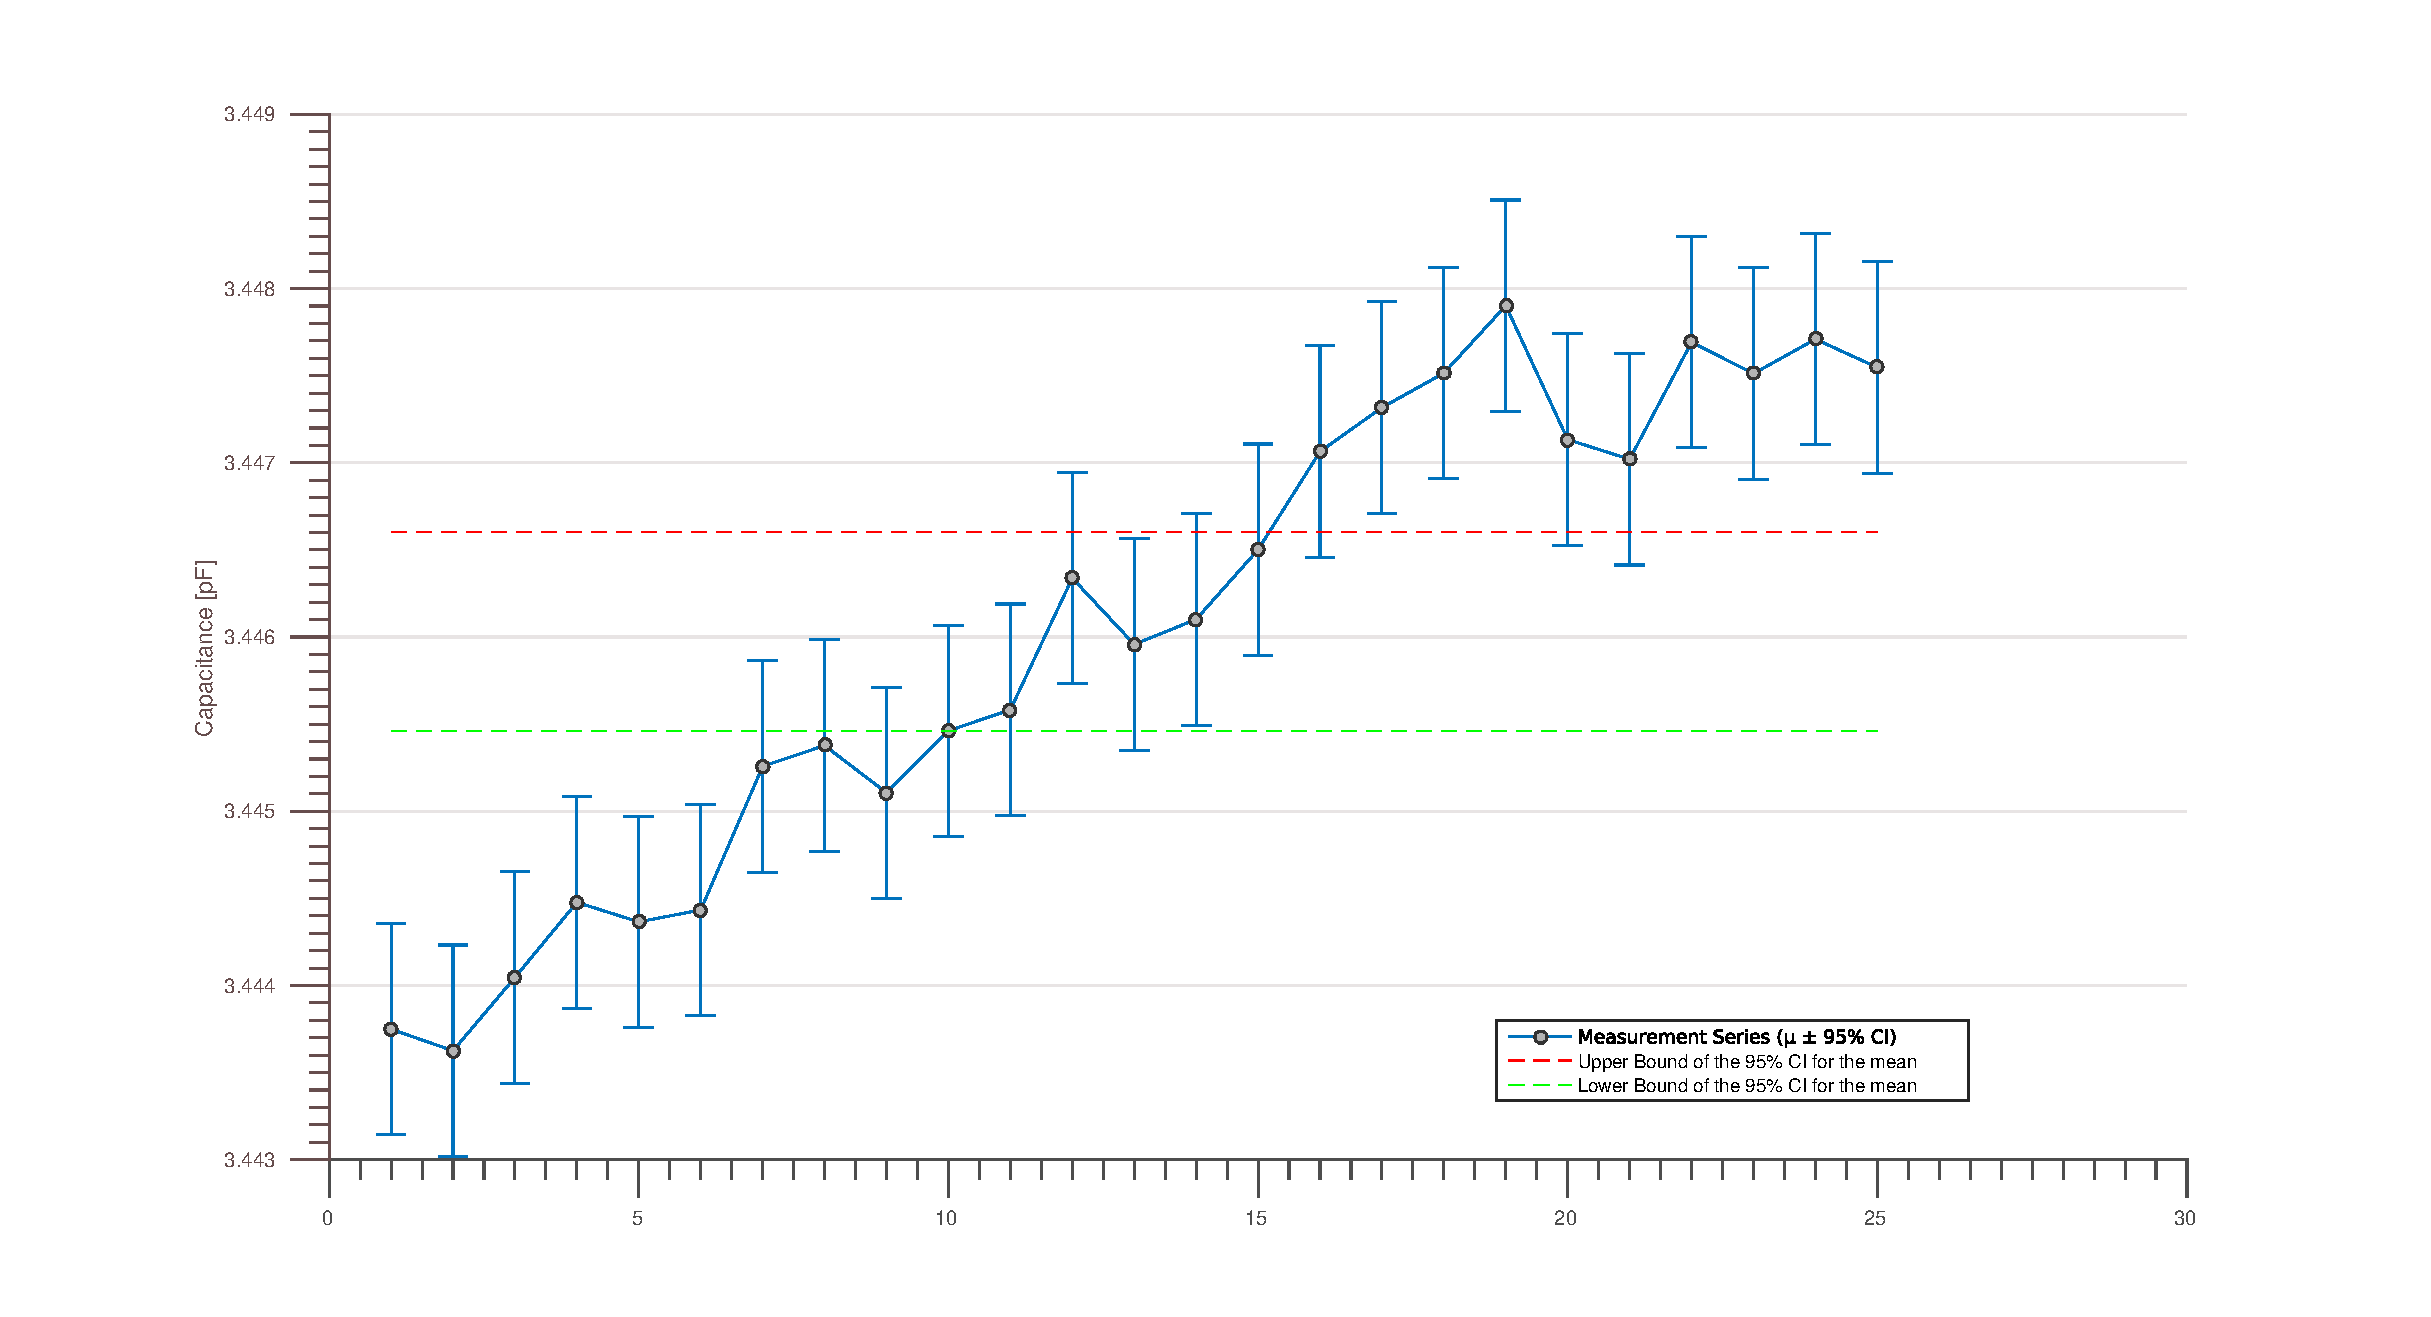
\includegraphics[scale=0.3]{figures/Results/Capacitance_Measure/capacitanceplot.eps}		
	\caption[Kurze Abbildungsbeschreibung]{Measurements of sample capacitance for a series of re-insertions} 
	\label{fig.messreihe}
\end{figure}

The graph \ref{fig.messreihe} effectively contains two measurement series in one. Each one of the gray points represents one measurement in which
the setup was not changed and 25 phase averages were recorded. The resulting confidence interval is depicted by the error bar at each points
and amounts to about 1.12 fF.
\newline
Different gray points were measured by taking out the sample from its container and re-inserting in order to estimate how the results vary in that case.
It turned out that this lead to a much larger measurement variance. Moreover a increase in the capacitance value for each new re-insertion was detected.
And the series of 25 measurements is not enough to predict whether or not if and when the measurements are going to converge, so instead of the maximum difference of
5fF throughout the measurement, a maximum variance of 10fF was assumed.
\newline
For determining the distance, the 
effective dielectric permittivity is assumed to be known. When
considering a maximum electrode distance of 0.25 mm and linearizing the mistake around that point, the 10fF inaccuracy
when measuring the capacitance accounts to about a 11.3 $\mu$m when consulting the look-up table.
The average of the measurements for the magnitude of specimen capacitance amounts to
\begin{equation}
 C_{spec}=3.446pF \pm 5fF
\end{equation}

After the measurement, the same specimen was sawed open in order to perform an optical measurement of the electrode distance.


\begin{figure}[ht]
	\centering
	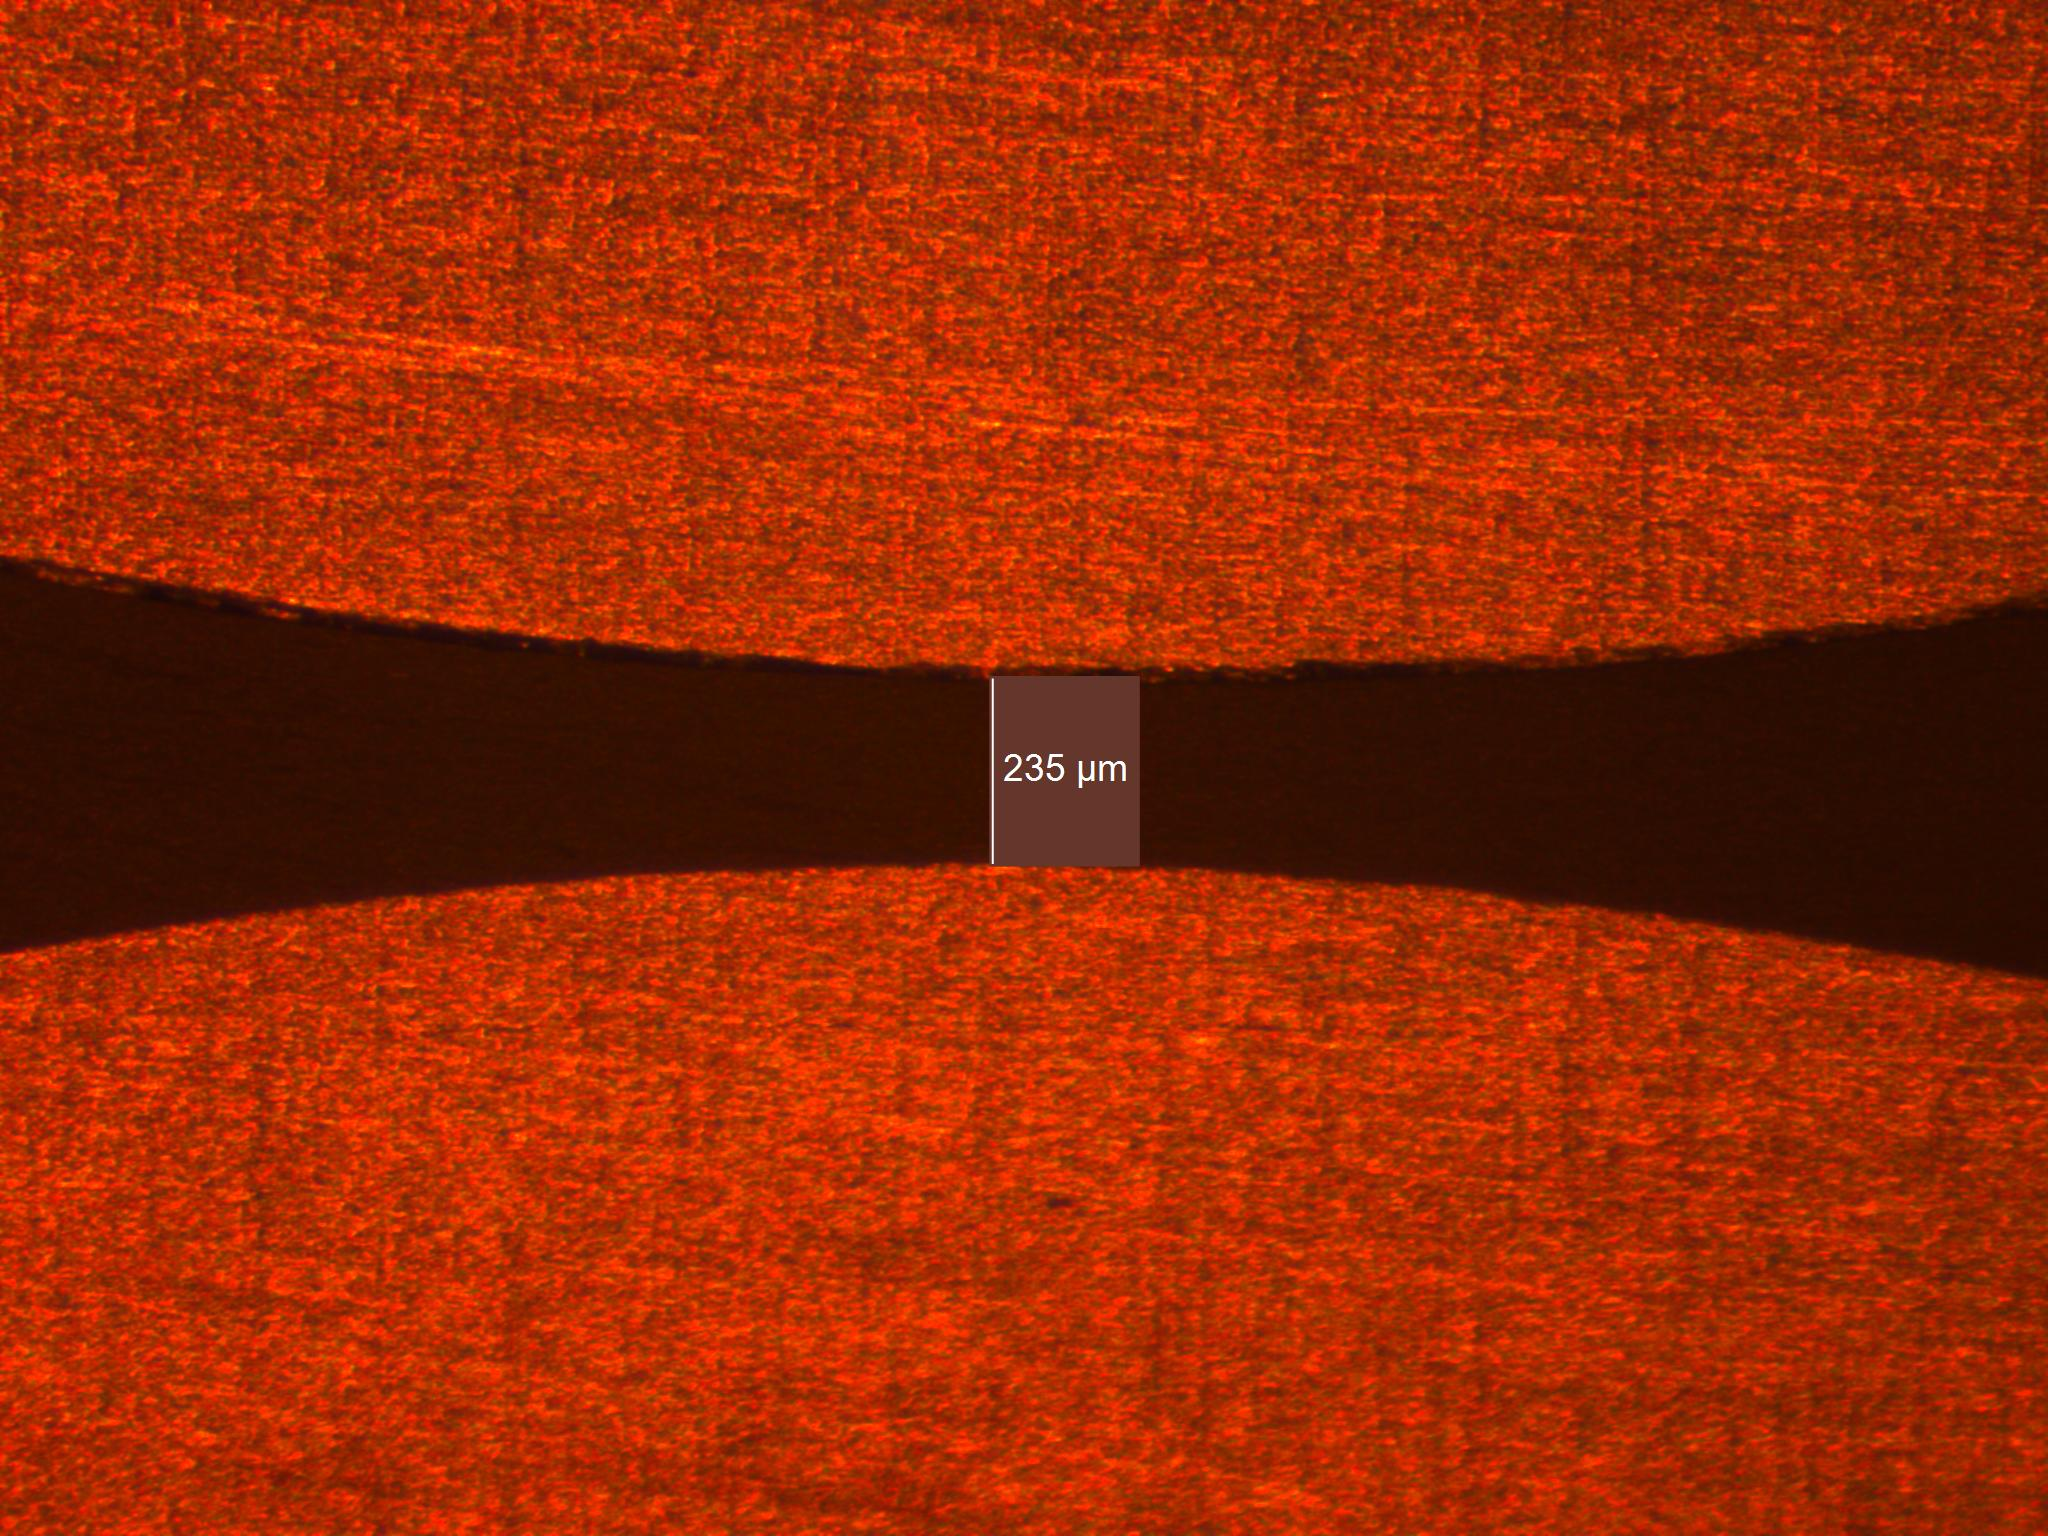
\includegraphics[scale=0.12]{figures/Results/Capacitance_Measure/Sample1_scale.jpg}		
	\caption[Kurze Abbildungsbeschreibung]{Measurements of sample capacitance for a series of re-insertions} 
	\label{fig.opticalmeasurement}
\end{figure}

Using the measured capacitance values in conjunction with the in \ref{fig.opticalmeasurement} determined distance and the look-up table
we find the effective relative permittivity to be:

\begin{equation}
 \epsilon_{eff}=3.85 \pm 0.05
\end{equation}


\section{Current transformer and protective clamping} 
As it was mentioned in the previous chapters, the main advantage to use a current transformer for
dielectric spectroscopy is the fact that the measurement equipment is galvanicaly insulated from the high-voltage supply and its
coupling in case of object breakdown. The analysis of how the current transformer behaves in this case is being conducted in this section.
The peak of the pulses that simulate the breakdown current from the capacitor bank were set to anywhere between 25A and 100A and its duration was about 7 $\mu$s.
The first two experiments were conducted without the protective TVS-Diodes that would limit the ouptut voltage.
The blue curve represents the current through the transformer. The blue line shows how much voltage is applied to a 10 m$\Omega$ shunt resistor and from this information the current can
be deducted. The red line depicts the voltage of the current transformer. To understand the red lines scale, one must consider that firstly, a -40 dB attenuator was placed in front the
oscilloscope and the measurement line was terminated with 50 Ohms, which implies that the real voltage is twice as high as the red curve suggests. For that reason the scale of the red measurement was half the size in order to illustrate the
$\frac{1V}{1A}$ characteristic of the current transformer when taking the blue line as a reference.
\newline 
This leads to the fact that 100mV on the blue scale amount to 10A of current and 10V at the output of the current transformer and the graphs \ref{fig.26Anodiode} to \ref{fig.comparison} should be interpreted
this way.


\begin{figure}[!ht]
	\centering
	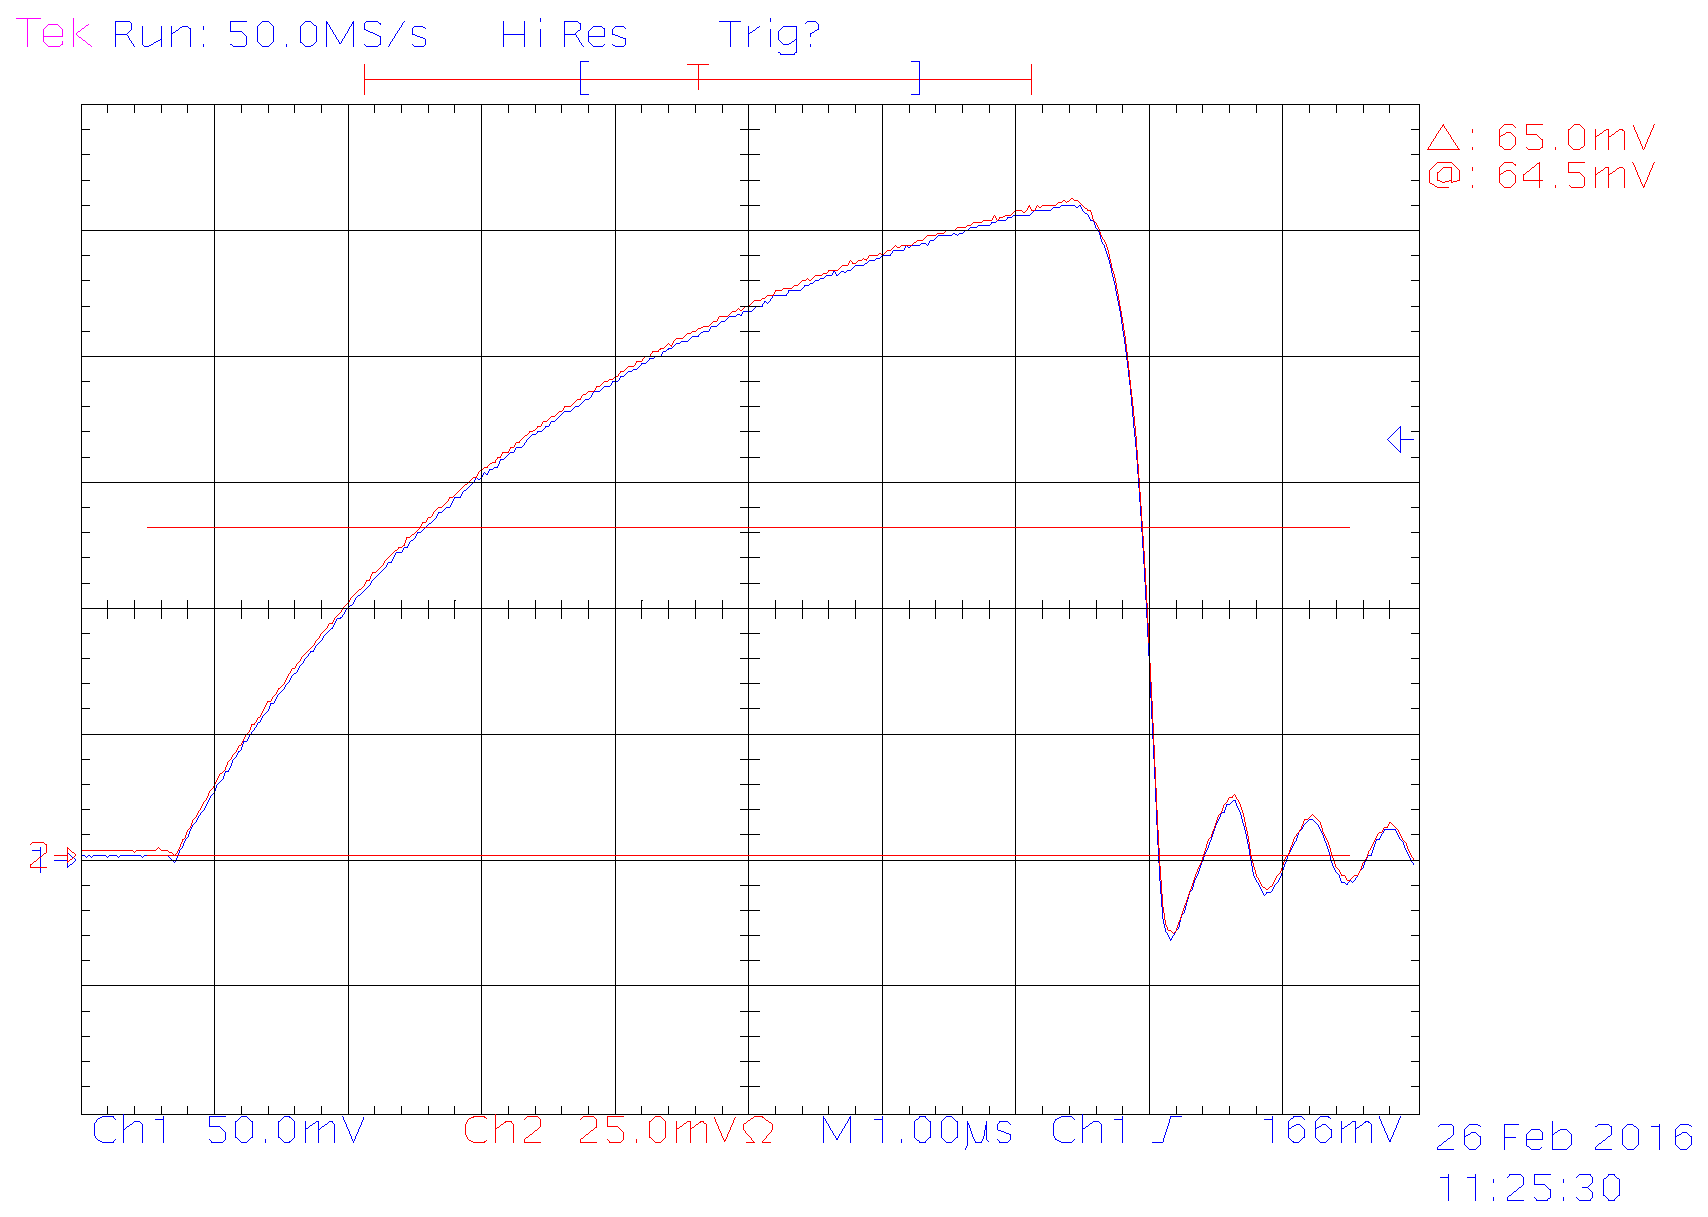
\includegraphics[scale=0.3]{figures/Voltage_Clamping/TEK00001.eps}		
	\caption[Kurze Abbildungsbeschreibung]{26A peak current pulse and no TVS-Diode with resulting voltage} 
	\label{fig.26Anodiode}
\end{figure}

\begin{figure}[!ht]
	\centering
	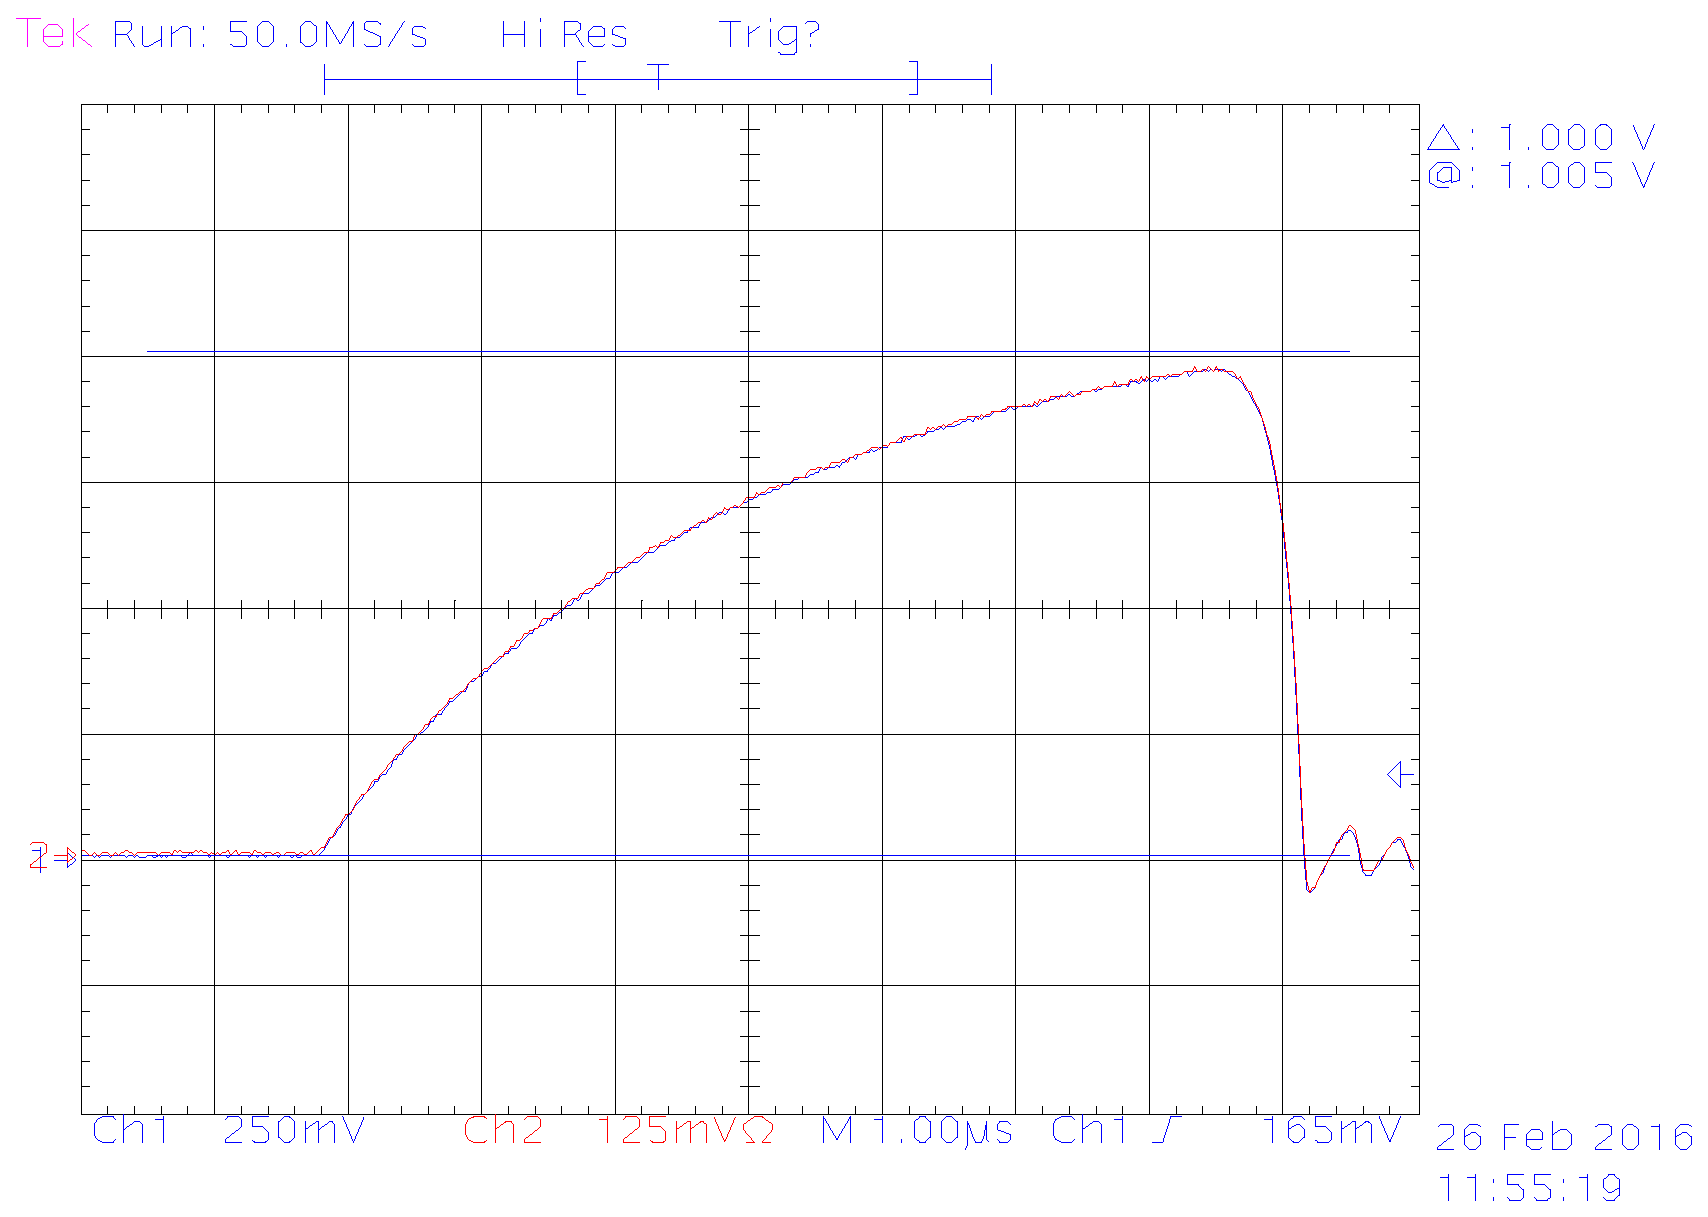
\includegraphics[scale=0.3]{figures/Voltage_Clamping/TEK00004.eps}		
	\caption[Kurze Abbildungsbeschreibung]{95A peak current pulse and no TVS-Diode with resulting voltage} 
	\label{fig.100Anodiode}
\end{figure}

Judging from the graphs \ref{fig.26Anodiode} and \ref{fig.100Anodiode}, the voltage generated by the current transformer aligns almost
perfectly with the current from the capacitor bank.

\begin{figure}[!ht]
	\centering
	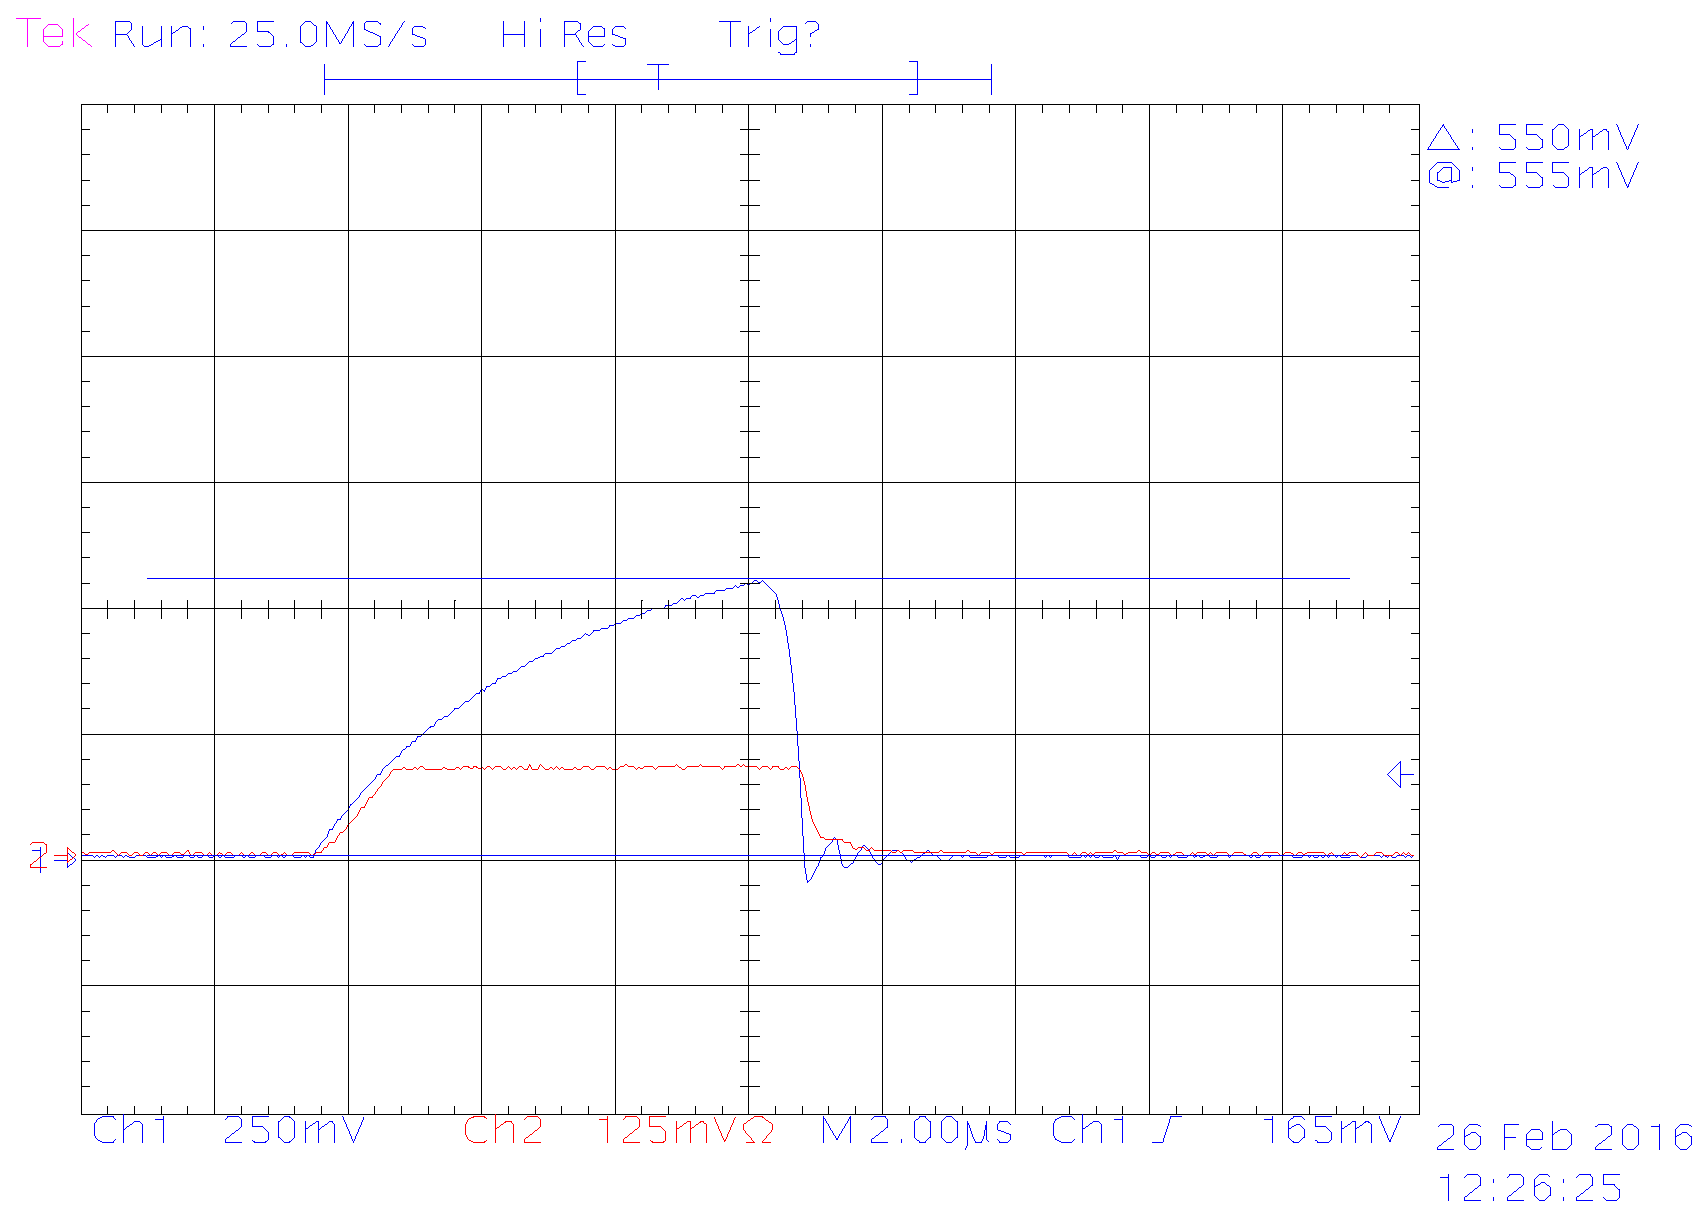
\includegraphics[scale=0.3]{figures/Voltage_Clamping/TEK00006.eps}		
	\caption[Kurze Abbildungsbeschreibung]{53A peak current pulse and inserted TVS-Diode with resulting voltage} 
	\label{fig.53Adiode}
\end{figure}

\begin{figure}[!ht]
	\centering
	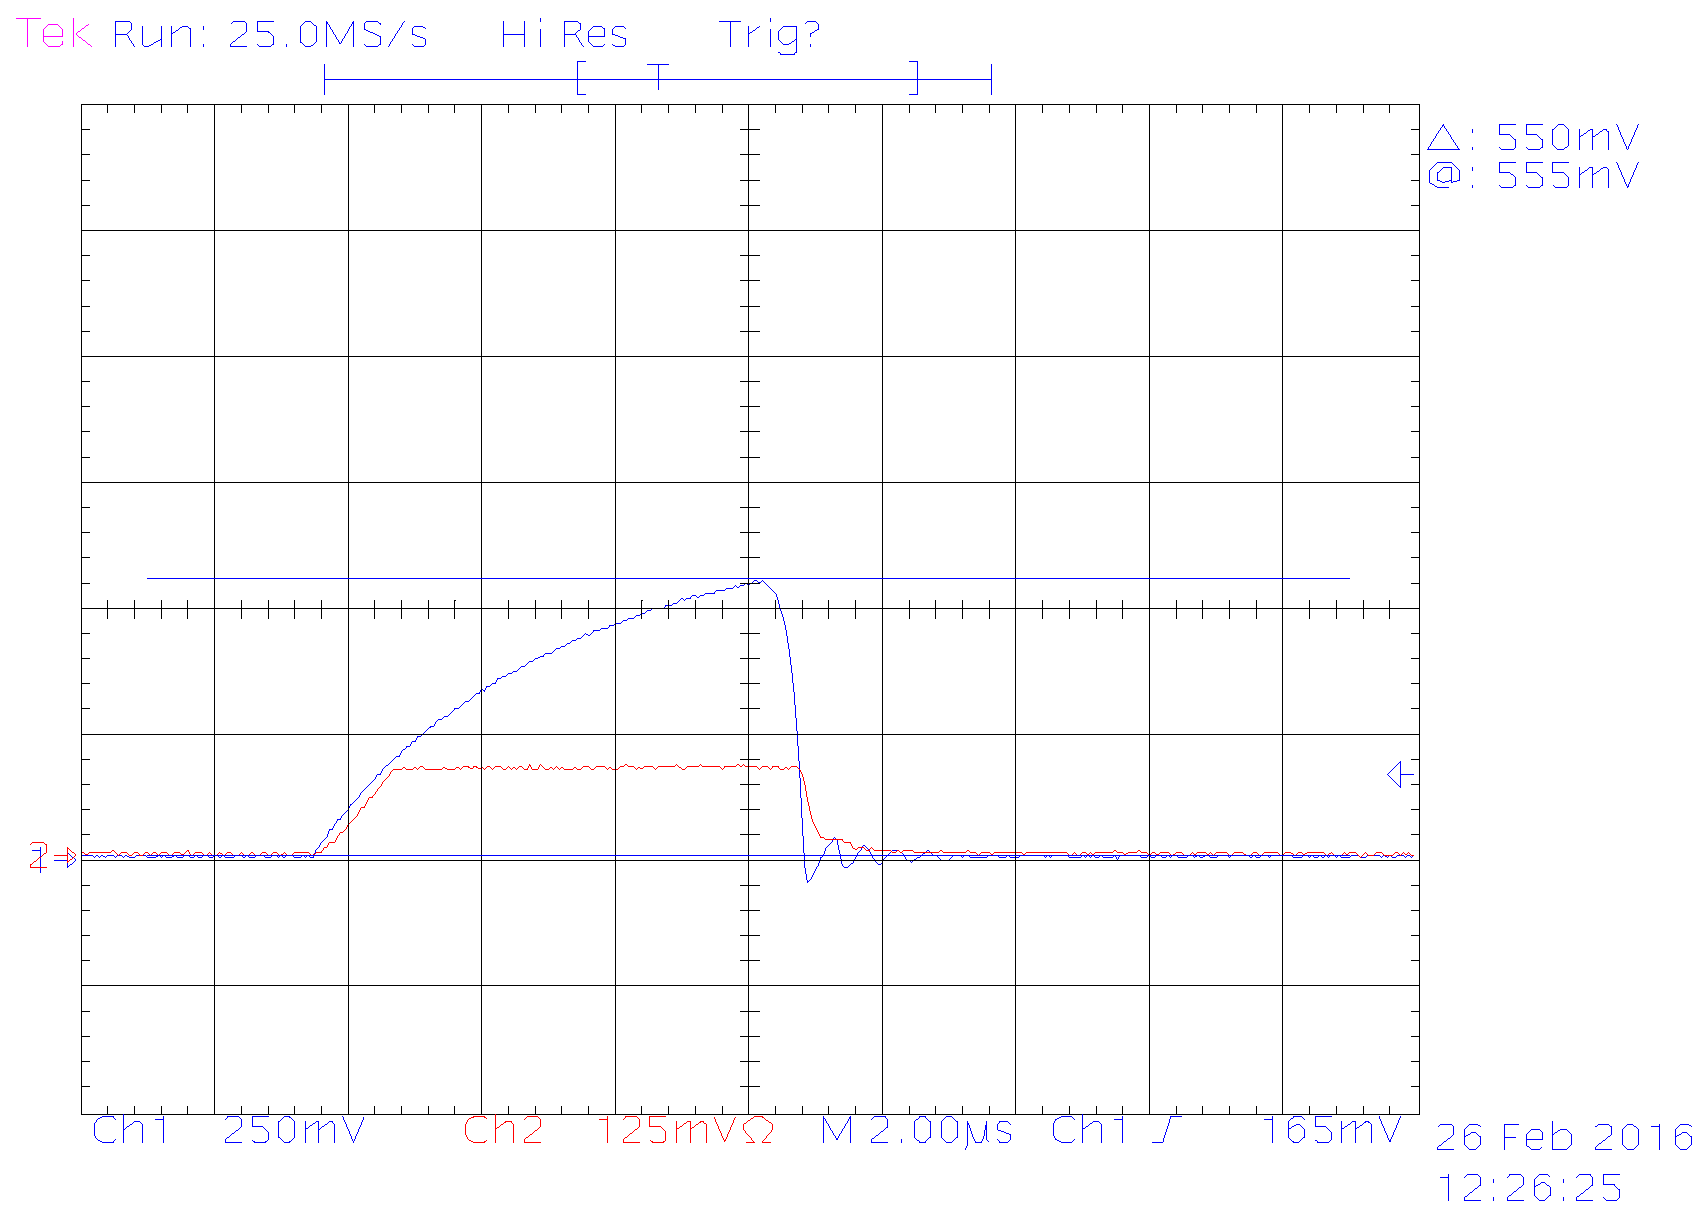
\includegraphics[scale=0.3]{figures/Voltage_Clamping/TEK00006.eps}		
	\caption[Kurze Abbildungsbeschreibung]{102A peak current pulse and inserted TVS-Diode with resulting voltage} 
	\label{fig.100Adiode}
\end{figure}

The recorded current and voltage from \ref{fig.53Adiode} and \ref{fig.100Adiode} show on
one hand that the protective diodes reliably clamp the voltage once it would normally go above 17.5 V even
independent of how high the actual current throught the current tranformer is. But on the other hand, the signals are no longer as similar as they were 
without the clamping.


This fact becomes even more apparent when we analyze currents that do not result in a voltage above the clamping voltage.
In figure it can be noticed how the red curve struggles to follow the current and even in the oscillation part at the end a remarkable phase shift was detected which results in a significant
mistake.


\begin{figure}[ht]
	\centering
	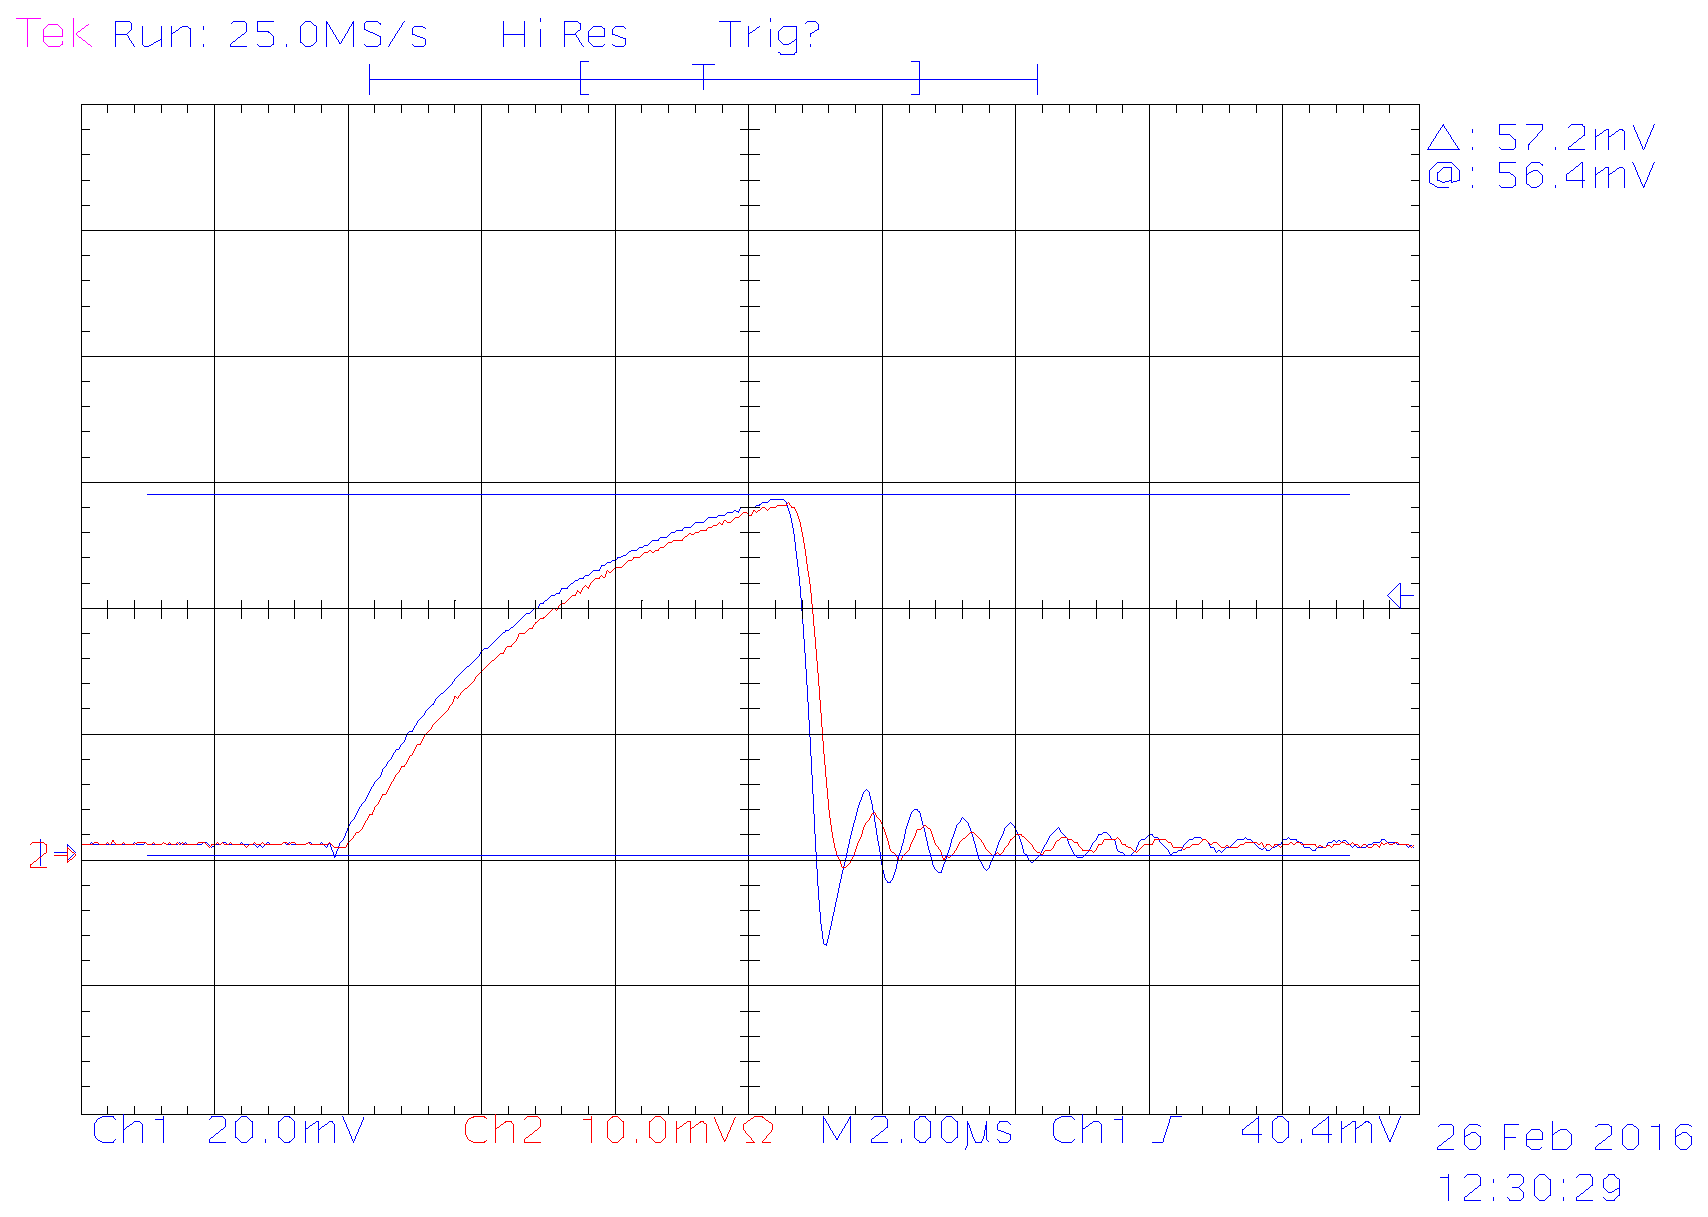
\includegraphics[scale=0.3]{figures/Voltage_Clamping/TEK00008.eps}		
	\caption[Kurze Abbildungsbeschreibung]{5.8A peak current pulse and inserted TVS-Diode with resulting voltage (no clamping)} 
	\label{fig.comparison}
\end{figure}

\section{Dielectric Spectroscopy}
\subsection{Loss tangent}
\begin{figure}[htbp]
  \centering
  \centerline{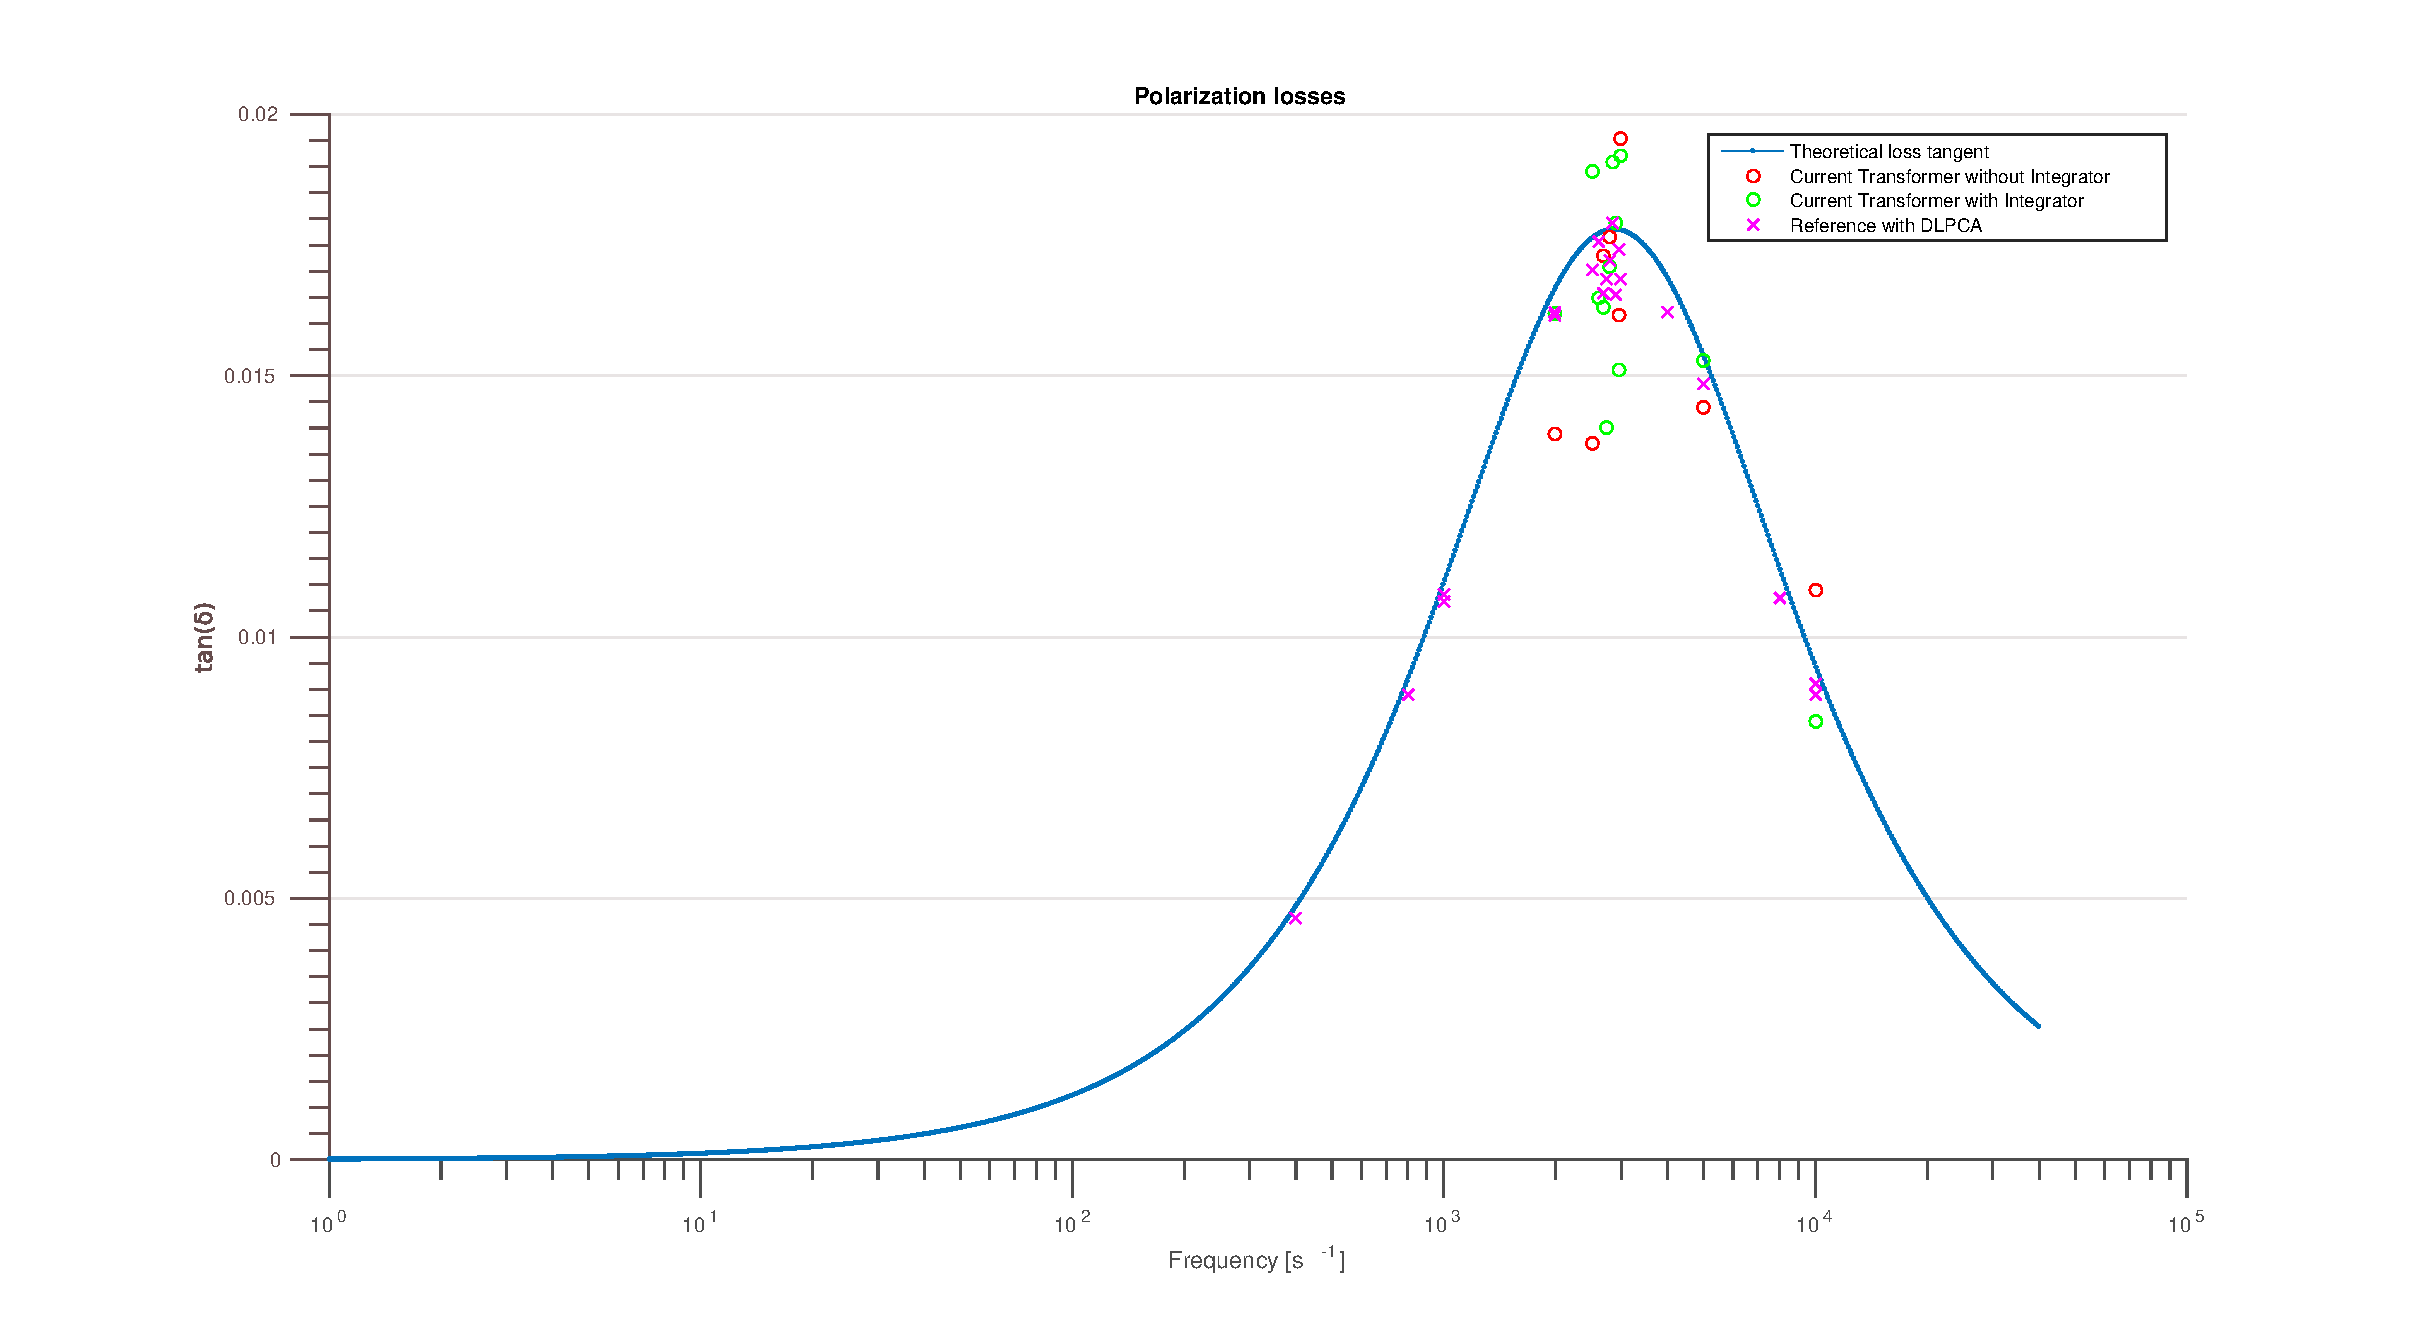
\includegraphics[scale=0.3]{figures/Results/Spectroscopy/spectroscopywithoutbars}}
  \caption[Kurze Abbildungsbeschreibung]{Measurements of dielectric loss tangent in different setup configurations}

  \label{fig.spectroscopy}

\end{figure}
The three data series created from the spectroscopy experiment using the Debye model are shown in the graph above. The solid blue line represents the theoretical  dielectric loss tangent given the parameters of the components in the debye model
as a function of the frequency.
The components were assumed to be ideal and not to be temperature dependent.
The magenta data points can be used as a reference to evaluate the performance of the current transformer as these measurement points
were obtained with a industry standard low-noise current amplifier (DLPCA). 
The red points were recieved by replacing the DLPCA with the current transformer.
The green points were measured with the integrator in place, effectively integrating the voltage signal generated by the current transformer.

\begin{figure}[htbp]
 \centering
 \centerline{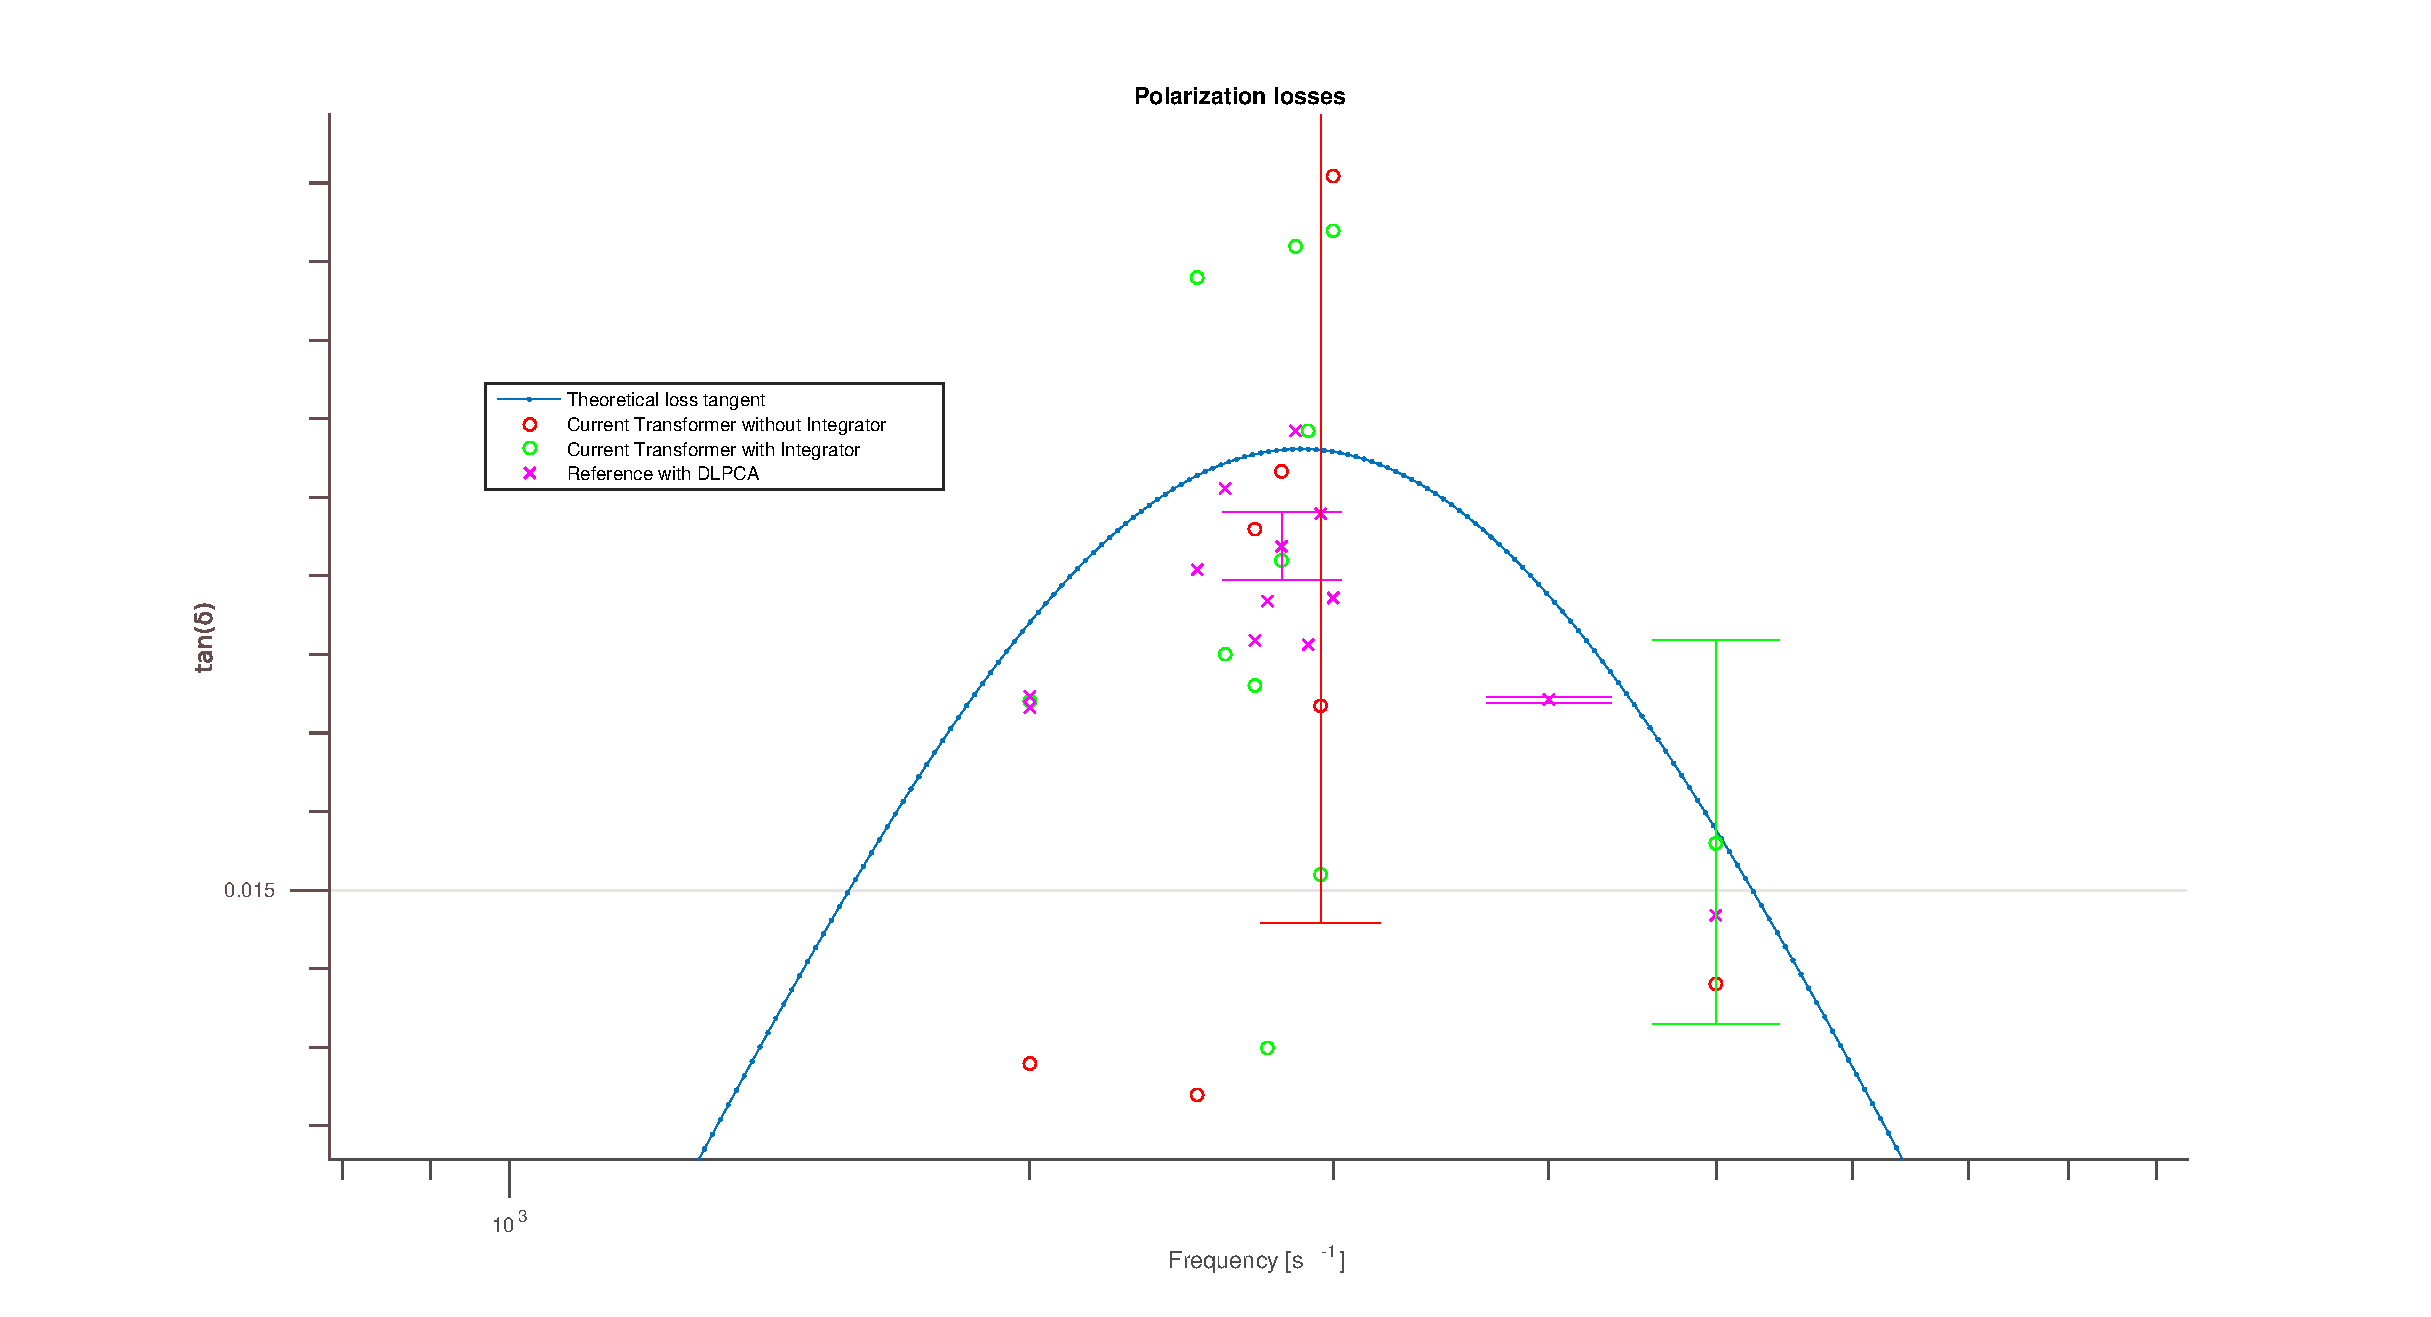
\includegraphics[scale=0.3]{figures/Results/Spectroscopy/errorbarsbettercolor}}

\caption[Kurze Abbildungsbeschreibung]{Confidence intervals}
\label{fig.spectroscopy2}
\end{figure}

In order to adequately analyze the data points, the above graphic shows the previous plot
zoomed in around the maximum loss tangent since the deviation from the theoretical result seem to be the largest here.
The confidence intervals were added for a few points in each measurement series.

First it can be noted that while the reference measurements fit the curve the closest, the theoretical values are still not
within the measurements confidence intervals and the error can be greater than 10\%. To sum up the measurements conducted with
the current transformer, it can be stated that the measurement performance was significantly worse than the reference. Not only do they deviate further from the theoretical values
but they also have a larger variance. Which means that one cannot consistently predict a reasonable range for the mean of said measurement, at least not for only 9 phase averages.
While the use of the integrator succesfully lowered the deviation and shrinked the confidence intervals by a factor of 2 to 3, the measurement accuracy is still nowhere close to the one obtained with the DLPCA.

\subsection{Analysis of Noise Parameters}

In order to identify one of the sources to which the errors can be attributed, the noise level at the input and at the ouput was measured and analyzed to gain an estimation about how much noise was added in the system.
Using the current transformer in both configurations, i.e. with and without the integrator, the following parameters were measured. They will be put in perspective when comparing them to the first table that includes the same quantites for the DLPCA setup.


\textit{Data for the DLPCA:}


\begin{center}
\begin{tabular}{|m{3cm}|m{3cm}|m{2.5cm}|m{3.2cm}|m{2cm}|} 
\hline
frequency [Hz]& SNR$_{in}$ & SNR$_{out}$ & Noise Figure [dB] & Noise Floor \\ 
\hline \hline
2000 &  8.25E+06 &  3.74E+05 & 13.43 & 1.00E-05 \\ 
\hline
2500 & 6.95E+06 & 6.02E+05 & 10.62 & 1.00E-05 \\ 
\hline
2700 & 3.92E+05 & 2.19E+05 & 2.53 & 1.00E-05 \\ 
\hline
3000 & 6.5E+04 & 4.72E+04 & 1.39 & 1.00E-05 \\ 
\hline
5000 & 2.331E+06 & 4.40E+06 & 2.76 & 1.00E-05 \\ 
\hline
\end{tabular}
\end{center}


\textit{Data without integrator:}
\begin{center}
\begin{tabular}{|m{3cm}|m{3cm}|m{2.5cm}|m{3.2cm}|m{2cm}|} 
\hline
frequency [Hz]& SNR$_{in}$ & SNR$_{out}$ & Noise Figure [dB] & Noise Floor \\ 
\hline \hline
2000 & 2.40E+07 & 16.31 & \cellcolor{blue!25}61.79 & 1.00E-05 \\ 
\hline
2500 & 1.8E+07 & 25.69 & \cellcolor{blue!25}58.55 & 1.00E-05 \\ 
\hline
2700 & 5.10E+07 & 31.02 & \cellcolor{blue!25}42.23 & 1.00E-05 \\ 
\hline
3000 & 5.13E+05 & 42.04 & \cellcolor{blue!25}40.86 & 1.00E-05 \\ 
\hline
5000 & 7.17E+06 & 79.386 & \cellcolor{blue!25}49.56 & 1.00E-05 \\ 
\hline
10000 & 1.09E+06 & 377.35 & \cellcolor{red!25}34.616 & 1.00E-04 \\ 
\hline

\end{tabular}
\end{center}

\textit{Data with integrator:}
\begin{center}
\begin{tabular}{|m{3cm}|m{3cm}|m{2.5cm}|m{3.2cm}|m{2cm}|} 
\hline
frequency [Hz]& SNR$_{in}$ & SNR$_{out}$ & Noise Figure [dB] & Noise Floor \\ 
\hline \hline
2000 & 3.00E+07 & 35.23 & \cellcolor{blue!25}59.35 & 1.00E-05 \\ 
\hline
2500 & 1.77E+07 & 78.12 & \cellcolor{blue!25}53.5 & 1.00E-05 \\ 
\hline
2700 & 3.60E+05 & 39.05 & \cellcolor{blue!25}40.6 & 1.00E-05 \\ 
\hline
3000 & 3.17E+05 & 113.1 & \cellcolor{blue!25}34.47 & 1.00E-05 \\ 
\hline
5000 & 8.90E+06 & 23.44 & \cellcolor{blue!25}41.7 & 1.00E-05 \\ 
\hline
10000 & 1.10E+06 & 22.5 & \cellcolor{red!25}46.9 & 1.00E-04 \\ 
\hline

\end{tabular}

\end{center}
When a sinusoidal input is applied to the system. The SNR was defined as the ratio of the energy in the FFT-bin that corresponds
to the fundamental frequency of the oscillation and the energy of all other components. Since the distance of the sampling in the time domain was chosen
such that the first index shows the proportion of the fundamental frequency in the signal, the signal to
noise ratio can be defined as follows.


\begin{equation}
SNR=\frac{\hat{x}[1]^2}{\sum\limits_{i=0,i\neq1}^{N}\hat{x}[i]^2}
\end{equation}

The noise figure relates the noise level at the input and the output and therefore is a measure of the added noise of the measurement setup:

\begin{equation}
 Noise\,Figure\, [dB]=10log\left(\frac{SNR_{in}}{SNR_{out}}\right)
\end{equation}

Noise floor is a parameter that declares around which value the spectral components of the higher frequencies, i.e. noise are located. Generally it can be said that the higher the noise floor is,
the higher the variance in the measurement of the dielectricl loss tangent.\cite{FaerberMVISS}
When using the current transformer, it has to be taken into account that between the frequencies of 2000 Hz up to 5000 Hz, a degradation of the noise
figure of about 40-50 dB has to be expected. However one must consider that the DLPCA used a variable gain in order to generate an output whose amplitude amounts to about 10V which takes advantage of the full resolution of the 
digital to analog converter, whereas in the other two setups the gain was set to a constant value.
The noise figure does in fact decrease when the integrator is in use. Yet, most likely due to the non-idealities described in the next section, the noise figure varied within 5dB for the same frequency. 
The calculated values for the noise figure for the setup with integrator were still consistently lower than the one for the setup without it for frequencies up to 5000 Hz.

The following figures illustrate the spectral distribution of the noise for 2000 Hz at the output for a sinusoidal input. Using these graphs, the above mentioned value for the noise floor can be determined.


\begin{figure}[htbp]
 \centering
 \centerline{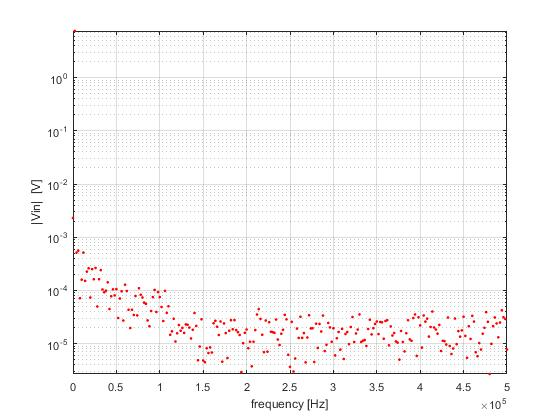
\includegraphics[scale=0.3]{figures/Results/NoiseFloor/DLPCA.jpg}}

\caption[Kurze Abbildungsbeschreibung]{Noise Floor of Measurement with DLPCA }
\label{fig.noisefloordlpca}
\end{figure}

\begin{figure}[htbp]
 \centering
 \centerline{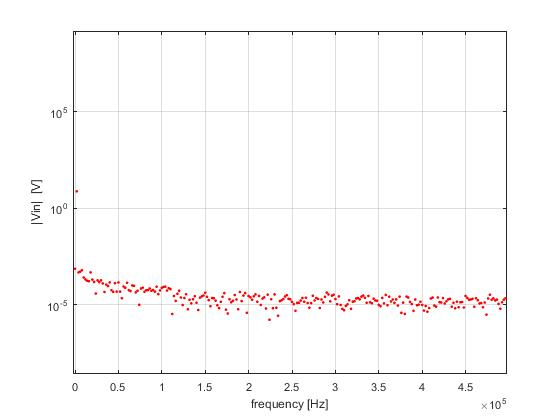
\includegraphics[scale=0.3]{figures/Results/NoiseFloor/currenttransformer.jpg}}

\caption[Kurze Abbildungsbeschreibung]{Noise Floor of Measurement with current transformer }
\label{fig.noisefloorcurrentt}
\end{figure}

\begin{figure}[htbp]
 \centering
 \centerline{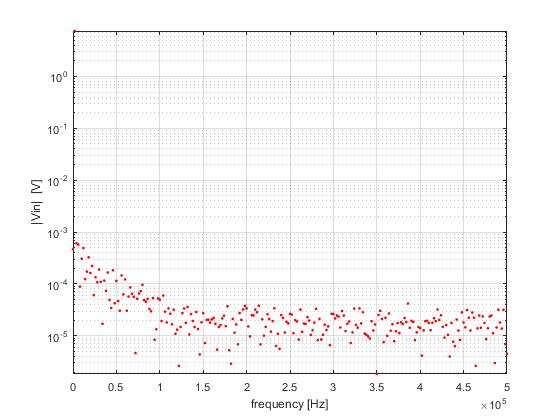
\includegraphics[scale=0.3]{figures/Results/NoiseFloor/Integrator.jpg}}

\caption[Kurze Abbildungsbeschreibung]{Noise Floor of Measurement with current transformer and integrator }
\label{fig.noisefloorintegrator}
\end{figure}




\section{Performance of integrator}
As described in the previous two passages, the integrator was capable of reducing the noise figure and hence effectively reducing 
the confidence interval when determining the dielectric loss tangent. While measuring the output of the integrator, particularily two unexpected problems were determined.
First, a DC offset at the output, that was varying with different input signals was detected. For an applied voltage, that had the shape of the expected transformed current pulse train
flowing through the debye equivalent, this offset could not be eliminated by tuning the potentiometer at the operational amplifier.

\begin{figure}[htbp]
 \centering
 \centerline{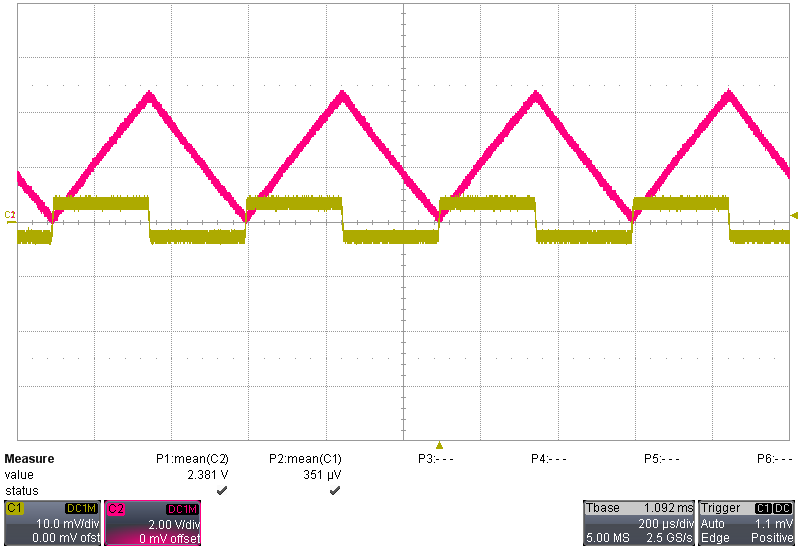
\includegraphics[scale=0.3]{figures/Results/Integrator_measurements/voltwave_10us}}

  \caption[Kurze Abbildungsbeschreibung]{Output in magenta applying a rectangular voltage signal with a rise time of 10 microseconds at the input}
\label{fig.voltwave_10us}
\end{figure}

Secondly, even when the same periodic signal was applied at the input of the integrator, a low frequency oscillation was imposed onto the output signal.
\begin{figure}[htbp]
 \centering
 \begin{minipage}{0.4\textwidth}
 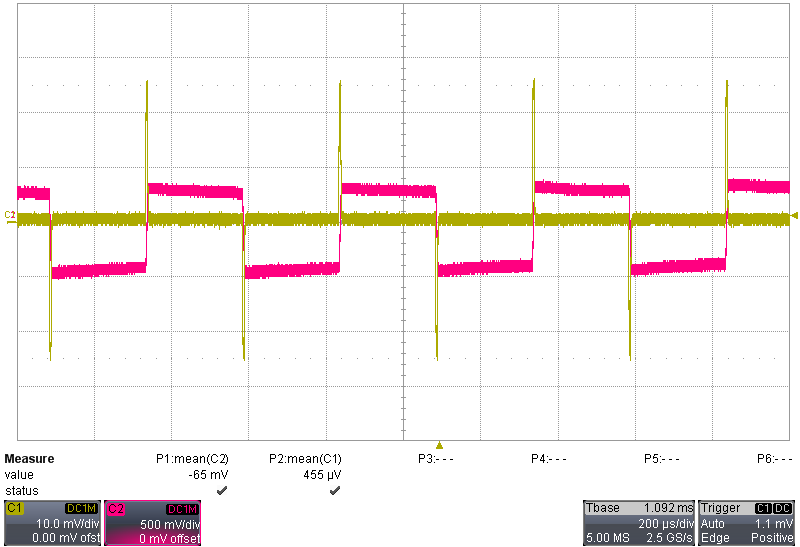
\includegraphics[scale=0.2]{figures/Results/Integrator_measurements/currentwave_10u}
 \caption[Kurze Abbildungsbeschreibung]{Applying the current pulse caused by a rectangular voltage signal with a rise time of 10 microseconds at one instant. }
 \end{minipage}\qquad
 \begin{minipage}{0.4\textwidth}
 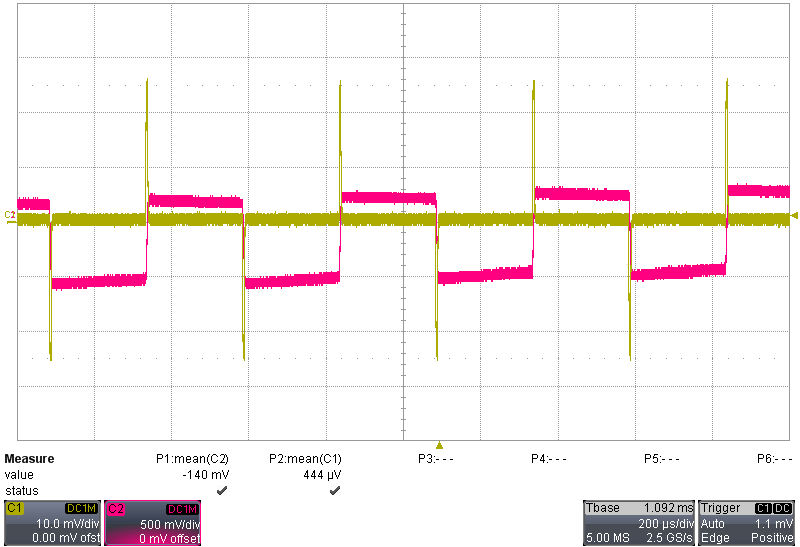
\includegraphics[scale=0.2]{figures/Results/Integrator_measurements/cuwave_10u-4}
 \caption[Kurze Abbildungsbeschreibung]{Applying the current pulse caused by a rectangular voltage signal with a rise time of 10 microseconds at another instant.}
 \end{minipage}
 
  
\end{figure}

For the purpose of estimating the extend of the low frequency noise, a FFT-analysis of the output was conducted while applying a sinusoidal input at 2000 Hz.

\begin{figure}[htbp]
 \centering
 \centerline{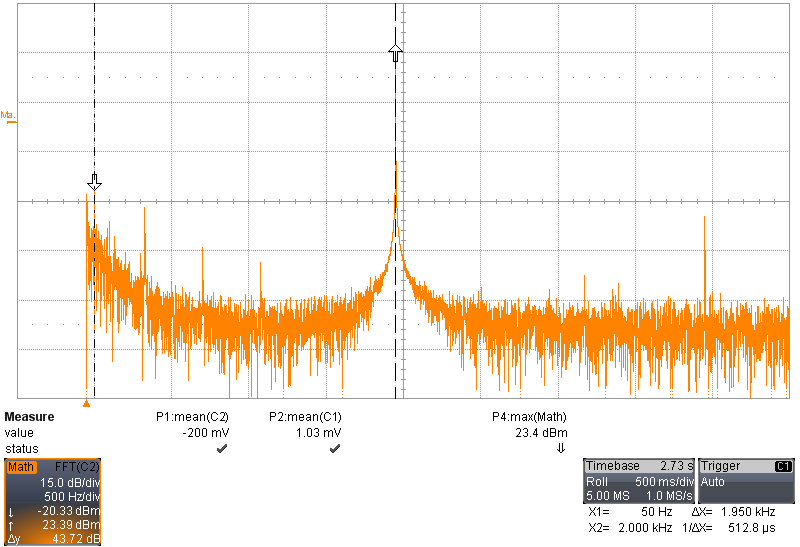
\includegraphics[scale=0.3]{figures/Results/Noisespectrum/sin2k-0_02v}}

  \caption[Kurze Abbildungsbeschreibung]{FFT-spectrum of integrated sine-wave at 2kHz}
\label{fig.noisefft}
\end{figure}

The spectral components of the lower frequencies in \ref{fig.noisefft} are relatively high when compared to the striking peak that can be attributed to the 2000 Hz fundamental frequency.
Furthermore, the amplitude of the lower frequencies is similar to the one of the first harmonic, i.e. 4000 Hz.
Judging from the results of this section, the two described non-idealities can not be neglected, the DC offset and the low frequency noise contribute significantly to the signal degradation and
most probably prevent the integrator from reducing the noise figure more considerably.


The following graph shows the influence or the air gap. 
\begin{figure}[htbp]
	\centering
	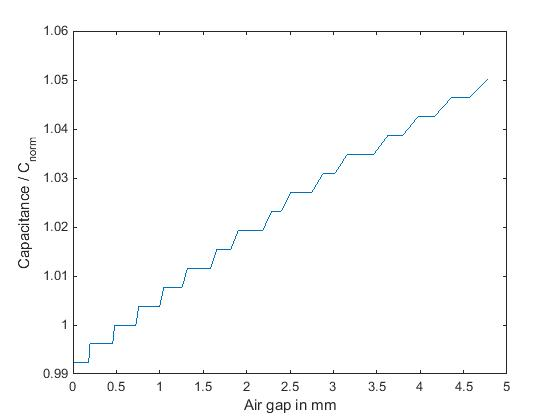
\includegraphics[width=0.5\textwidth]{figures/Results/airgap_height/airgap_graph.jpg}		
	\caption[Kurze Abbildungsbeschreibung]{Effect of a deviation of the air gap on the vacuum capacitance} \ref{fig.airgap}
	\label{fig.waveforms}
\end{figure}
 

The illustration of the height deviation proves that it is negligible and thus has no significant influence on the results. 
 \begin{figure}[htbp]
	\centering
	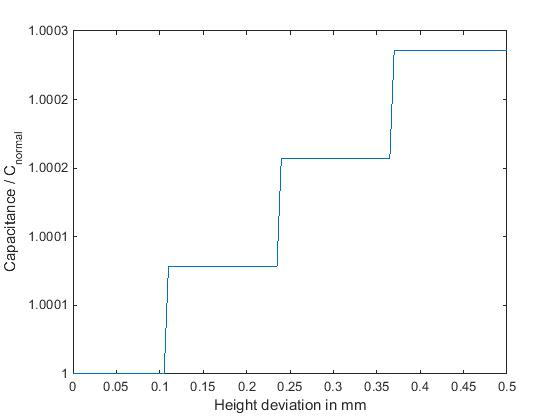
\includegraphics[width=0.5\textwidth]{figures/Results/airgap_height/Height_deviation.jpg}		
	\caption[Kurze Abbildungsbeschreibung]{Effect of a deviation in the height of the epoxid resin on the capacitance} \ref{fig.comsol_beispiel}
	\label{fig.waveforms}
\end{figure}
	%
	\chapter{Discussion}
The 
\begin{figure}[hbtp]
	\centering
	\psfragfig{figures/figure2}
	\caption{Ein Beispiel f�r psfragfig-Bilder}
\end{figure}


	%
	\chapter{Conclusions}
\section{Estimation of $\varepsilon$ of epoxy polymer}
The created lookup-table allows an estimation of the the electrode distance d.  As shown in the chapters before, other factors than the air gap can be neglected. The calculated correction factor allows to estimate the $\varepsilon$ of the expoxy polymer CY223 / HY 956 based on $\varepsilon_{\textrm{eff}}$ improves the estimation of $\varepsilon$. Thus, within the range of the created look-up table the aims of this part of the semester project were reached. 

It has to be noted that this method is based on the assumption that the initial $\varepsilon$ is always the same. This work did not investigate to what extent this assumption is tenable. 

\section{Statement on the suitability of the current transformer for dielectric spectroscopy}

The number of measured frequencies for the polarization losses is quite low, therefore, it would be useful to increase the number of input frequencies in order to validate whether the measured values approximately possess the shape of the function of tan($\delta$) over a larger area and how large the deviation from the theoretical value is. This necessitates an automation of the gain adaptation for the amplifier of the butter-worth filter in order to use the resolution scope of the ADC ($\pm 10V$)  effectively. 
The band of the confidence interval for polarization losses is approx. 48 \% of the midpoint's value. This indicates that the noise level with the present setup is too large to make an accurate estimation of the mean of the real loss tangent tan($\delta)$.







%%%%%%%%%%%%%%%%%%%%%%%%%%%%%%%%%%%%%%%%%%%%%%%%%%%%%%%%%%%%%%%%%%%%%%%%%%%%%%%%
%Verzeichnisse
%%%%%%%%%%%%%%%%%%%%%%%%%%%%%%%%%%%%%%%%%%%%%%%%%%%%%%%%%%%%%%%%%%%%%%%%%%%%%%%%

	\bibliographystyle{alpha} %sagt, wie das Literaturverzeichnis dargestellt und geordnet wird
%	\bibliographystyle{geralpha} % fuer entsprechende deutsche Bezeichnungen im Literaturverzeichnis wie bspw 'Seite' statt 'page'
	\bibliography{text/Literature} 	%hier muss der Name des .bib Files eingegeben werden aus dem Latex die Bibliographiedaten lesen soll

%%%%%%%%%%%%%%%%%%%%%%%%%%%%%%%%%%%%%%%%%%%%%%%%%%%%%%%%%%%%%%%%%%%%%%%%%%%%%%%%
%Anhaenge
%%%%%%%%%%%%%%%%%%%%%%%%%%%%%%%%%%%%%%%%%%%%%%%%%%%%%%%%%%%%%%%%%%%%%%%%%%%%%%%%

	
	
	\appendix
	
\chapter*{Eigenst�ndigkeitserkl�rung}

Diese Seite wird durch die Eigenst�ndigkeitserkl�rung ersetzt. 
	\chapter{Protocols}
\section{Protocol: Measurement of capacitance of two samples}
\large{Aim} \\
\begin{itemize}

\item Measurement of capacitances of two samples in order to derive the $\epsilon$ with a optically measured electrode distance 
\item Measurement of the deviation in capacitance due to slightly different insertion of the sample into the low-voltage cell. Measurement of the deviation in due to errors in the measurement devices. 
\item Optical measurement of electrode distance after curring the sample (done by Raphael F\"arber) 
\end{itemize}

\large{Used Instruments} 
\begin{itemize}
 \item Butterworth Filter: Alligator Technologies 
 \item DLPCA: 
 \item Oscilloscope: LeCroy
 \item External Voltage Supply: 
 \item DAC: National Instruments 

\end{itemize}


\large{Setup} \\
The input signal was  sinusoidal with 1kHz and $V_pp=16$. This signal is applied to two different samples in the low-voltage-setup. The current through the probe is measured with DLPCA, filtered with a Butterworth filter and then given to a ADC. 
Input signal and output current are measured and the division of these quantities allows to deduce $C*$.\\

Together with the optical measurement of d the effective $\epsilon$ can be calculated. 

Settings: \newline
Signal Generator:  sin, 1kHz, $V_pp=16V$
DLPCA:  automatically adapted gain
BW-Filter:  cutoff-frequency : 100kHz, Gain: 1

\large{Measurement} \\
25 measurements of the capacitance each time after the samples were taken out of the low-voltage cell and put in again. Each measurement comprises of 25 phase shifts. 

The measurements were conducted for two different samples.

Measured values for sample 2 is not usable as there is entrapped air near the electrode. This was realized when measuring the electrode distance after slicing of the sample.

\large{Surroundings} \\
Temperature: 
Humidity: 

\section{Protocol: Measurement of epsilon and tan(delta) of Debye Model}
\large{Aim} \\
\begin{itemize}
\item Measurement of the $tan(\delta)$ and $\epsilon$ for different frequencies beteween 1 kHz and 10kHz in order to compare the results with the theoretical values
\item  
\end{itemize}


\large{Used Instruments} 
\begin{itemize}
 \item Butterworth Filter: Alligator Technologies 
 \item DLPCA: 
 \item Oscilloscope: LeCroy
 \item External Voltage Supply: 
 \item DAC: National Instruments 

\end{itemize}


\large{Setup} \\
The input signal was  sinusoidal with 1kHz and $V_pp=15$. The signal is applied to the Debye-model in the low-voltage setup. The current through the Debye-model is firstly measured with DLPCA, filtered with a Butterworth filter and then given to a ADC. Secondly, just the current transformer is used to measure the current. Thirdly, the current transformer is used with an integrator. 
For all thre measurement setups the measurement is done with the complete Debye model and as a reference measurement just with $C_0$, i.e. $R_i$ and $C_i$ are removed. 

Settings: \newline
Signal Generator:  sin, 1kHz to10 kHz, $V_pp=16V$
DLPCA:  automatically adapted gain
BW-Filter:  cutoff-frequency : always double the input frequency, gain according to the following table

\large{Measurement} \\
Each time, 9 phase shifts were recorded. 

\large{Surroundings} \\
Temperature: 
Humidity: 


\section{Protocol: Measurement of Noise Figure and Noise Floor}
\large{Aim} \\
\begin{itemize}
\item Determination of the Noise figure with and without an integrator
\item Receiving noise flor 
\end{itemize}

\large{Surroundings} \\
Temperature: 
Humidity: 
%	\input{text/TechnischeZeichnungen}



\end{document}
